\documentclass[12pt, twoside, openright]{report}
\usepackage[utf8]{inputenc}
\usepackage{graphicx}
\usepackage[a4paper,width=150mm,top=25mm,bottom=25mm,bindingoffset=12mm]{geometry}
%\usepackage{biblatex}
\usepackage{setspace}
\usepackage[english]{babel} 
\usepackage{stmaryrd}
\usepackage{xcolor}
\usepackage{xspace}
%\usepackage{natbib}
\usepackage{csquotes}
\usepackage[style=apa, backend=biber]{biblatex}
%\DeclareLanguageMapping{american}{american-apa}
%\usepackage{apacite}
\addbibresource{references.bib}
\usepackage{tabularx}

% packages for reading results
\usepackage{pgfplotstable}
\usepackage{csvsimple}
\usepackage{siunitx}
\usepackage{lscape}
\usepackage{amsmath}

% define col width
\newcolumntype{Y}{>{\hsize=4\hsize}X}
\newcolumntype{s}{>{\hsize=0.25\hsize}X}
\graphicspath{ {images/} }

\linespread{1.25}
\counterwithout{footnote}{chapter}

\definecolor{Red}{RGB}{255,0,0}
\definecolor{Green}{RGB}{10,200,100}
\definecolor{Blue}{RGB}{10,100,200}
\definecolor{Orange}{RGB}{255,153,0}
\definecolor{Purple}{RGB}{139,0,139}

\newcommand{\denote}[1]{\mbox{ $[\![ #1 ]\!]$}}
\newcommand*\diff{\mathop{}\!\mathrm{d}}
\newcommand{\red}[1]{\textcolor{Red}{#1}}  
\newcommand{\mh}[1]{\textcolor{Blue}{[mht: #1]}}  
\newcommand{\mf}[1]{\textcolor{Orange}{[rl: #1]}}  
\newcommand{\js}[1]{\textcolor{Green}{[js: #1]}} 
\newcommand{\pt}[1]{\textcolor{Purple}{[pt: #1]}} 

% define functions for reading results from csv
\newcommand{\datafoldername}{R4Tex}

% the following code defines the convenience functions
% as described in the main text below

% rlgetvalue returns whatever is the in cell of the CSV file
% be it string or number; it does not format anything
\newcommand{\rlgetvalue}[4]{\csvreader[filter strcmp={\mykey}{#3},
	late after line = {{,}\ }, late after last line = {{}}]
	{\datafoldername/#1}{#2=\mykey,#4=\myvalue}{\myvalue}}

% rlgetvariable is a shortcut for a specific CSV file (myvars.csv) in which
% individual variables that do not belong to a larger chunk can be stored
\newcommand{\rlgetvariable}[2]{\csvreader[]{\datafoldername/#1}{#2=\myvar}{\myvar}\xspace}

% rlnum format a decimal number
\newcommand{\rlnum}[2]{\num[output-decimal-marker={.},
	exponent-product = \cdot,
	round-mode=places,
	round-precision=#2,
	group-digits=false]{#1}}

\newcommand{\rlnumsci}[2]{\num[output-decimal-marker={.},
	scientific-notation = true,
	exponent-product = \cdot,
	round-mode=places,
	round-precision=#2,
	group-digits=false]{#1}}

\newcommand{\rlgetnum}[5]{\csvreader[filter strcmp={\mykey}{#3},
	late after line = {{,}\ }, late after last line = {{}}]
	{\datafoldername/#1}{#2=\mykey,#4=\myvalue}{\rlnum{\myvalue}{#5}}}

\newcommand{\rlgetnumsci}[5]{\csvreader[filter strcmp={\mykey}{#3},
	late after line = {{,}\ }, late after last line = {{}}]
	{\datafoldername/#1}{#2=\mykey,#4=\myvalue}{\rlnumsci{\myvalue}{#5}}}

% MH's command
\newcommand{\brmresults}[2]{\(\beta = \rlgetnum{#1}{Rowname}{#2}{Estimate}{3}\) (\rlgetnum{#1}{Rowname}{#2}{l.95..CI}{3}, \rlgetnum{#1}{Rowname}{#2}{u.95..CI}{3})}
%\brmresults{expt1_brm.csv}{condition}

\begin{document}
\begin{titlepage}
	\begin{center}
		\vspace*{1cm}
		\Huge
		\textbf{Inferring Comparison Classes of Gradable Adjectives\\} 
		\vspace{0.5cm}
		\Large
		\textbf{The Role of Informational Goals and Sentence Structure}
		
		\vspace{1cm}
		
	
		\textbf{By \\ Polina Tsvilodub}
		
		\vspace{1cm}
		\small
		Submitted in partial fulfillment of the requirements for the degree of \\
		Bachelor of Science in Cognitive Science \\ to the \\
		Institute of Cognitive Science at the Osnabrück University\\
		September, X 2020
		
	%	\vfill
		\vspace{3cm}
		Thesis Supervisor:\\ Prof. Dr. Michael Franke, Institute of Cognitive Science, Osnabrück University \\
		\vspace{0.5cm}
		Thesis Supervisor:\\ Dr. Michael Henry Tessler, Postdoctoral Associate, Department of Brain and Cognitive Sciences, MIT  
		\vfill 
		
\includegraphics[width=0.6\textwidth]{unilogo.jpg}
		
	\end{center}
\end{titlepage}

\chapter*{Abstract}
Understanding gradable adjectives like “big” requires making reference to a so-called comparison class - a set of objects the referent is implicitly compared to. For example, the utterance “That Great Dane is big” could mean “That Great Dane is big compared to dogs in general” or “That Great Dane is big compared to other Great Danes”; yet the comparison class is rarely stated explicitly. So how do listeners establish the comparison class, given multiple a priori reasonable options?
Research on gradable adjectives has focused on the representation and integration of comparison classes into compositional semantics, but little is known about how human listeners decide upon a comparison class. 
This work takes a functional perspective on comparison class inference, guided by informational goals that speakers pursue when producing an utterance with a gradable adjective, and how listeners expect these goals to be achieved syntactically. For instance, given simple \textit{“Subject Predicate”} sentences listeners expect that the subject aids reference (i.e., identifies the target), whereas the predicate accomplishes predication (i.e., asserts a property of the subject). Therefore, a noun appearing in the predicate is more likely to be intended to constrain the comparison class, whereas a noun in the subject can be explained away as intended for reference, leaving comparison class inference to other pragmatic reasoning. 
Converging evidence from four behavioural experiments supporting this proposal is presented alongside a novel formalisation of the inferential account in a qualitative computational model within the Rational Speech Act framework. This work contributes to the body of research on gradable adjectives, and provides a case study of  context-dependent language, emphasizing the complexity of the relation between form and meaning of linguistic expressions. 


\chapter*{Acknowledgements}
%I want to thank...

The opportunity for this work to happen would not have been possible without the trust of three people. I want to thank Roger Levy for providing me the chance to visit the Computational Psycholonguistics Lab at MIT and accomplish my internship abroad. I would also like to state my infinite gratitute to Michael Henry Tessler for his feedback, the great deal of time and patience he invested in trusting me to work on this project during the internship, and to Michael Franke for his invaluable support and guidance through this thesis. It was also his trust that provided the opportunity for me to be a part of this project. Furthermore, I would like to thank Carina Kauf, Maximilian Gartz, Berit Reise and XXX for their feedback on this work. Finally, I would like to thank the anonymous reviewers and the audience at CogSci 2020 for their insightful comments and questions. 


\tableofcontents
%\listoffigures
%\listoftables

\chapter{Introduction}
\label{chapter01}
The meaning of natural language expressions heavily depends on the context in which these expressions are used, but speakers rarely explicitly outline which aspects of the context are relevant for their interpretation. 

This issue is clearly illustrated by utterances involving gradable adjectives like \textit{big, small, tall, expensive} etc. These adjectives are typically taken to describe a degree to which an object possesses some property, e.g., the degree of bigness (i.e., size), for the adjective ‘big’, but specific degrees a speaker intends to convey vary a lot depending on the particular referent and context. Intuitively, the utterance “That’s big!” denotes quite different size degrees, depending on whether it was uttered in reference to a flower or in reference to a house, while both objects could potentially co-occur in the same perceptual context; given this utterance, it is left to the listener to identify the correct referent and size degree. The aspect that goes unsaid and allows for this flexible use of the adjective \textit{big} across referents and contexts is \textit{what the intended referent is big relative to}. Humans easily infer that these two objects might be compared to different things: for instance, it is more likely that the flower is big for this specific kind of flowers or relative to other flowers around it, whereas the house is probably rather being compared to other houses in the neighborhood. 

However, speakers rarely explicitly state this comparison class - the set of entities the target is compared against, and it is left to the addressee to establish the relevant comparison set \parencite{Solt2009}. Listeners feature vast general knowledge and experience about the world helping them interpret context-sensitive language \parencite{tessler2017warm}, but what additional linguistic features do listeners attend to? In particular, how do listeners establish a comparison class in order to interpret a gradable adjective, given infinitely many a priori plausible options for the comparison class? 

This work investigates the role of syntactic structure for sentences containing relative gradable adjectives, suggesting that the syntax provides a cue to contextually relevant aspects for adjective interpretation, which is integrated with other cues like perceptual context and world knowledge.  \footnote{This thesis summarizes and extends the work by Tessler, Tsvilodub, Snedeker and Levy published in \textcite{tessler2020}, that appeared in the \textit{Proceedings of the 42nd Annual Meeting of the Cognitive Science Society}.} In particular, we hypothesize that syntactic structure reflects informational goals interlocutors strive to achieve; they reason about these goals pragmatically when inferring the comparison class of gradable adjectives. Focusing on the informational goals \textit{reference} and \textit{predication}, this work presents a novel \textbf{reference-predication trade-off hypothesis} of comparison class inference, contributing to the body of research on gradable adjectives and providing a case study for the relationship between linguistic form and meaning. Evidence from four behavioral experiments is provided in support of this functional hypothesis, as well as a Bayesian model of gradable adjective interpretation, showing that sophisticated pragmatic reasoning about syntactic structure can be captured using the generic probabilistic Rational Speech Act framework \parencite{goodman2016}. 
	


\chapter{Understanding Gradable Adjectives}
\label{chapter02}
Gradable adjectives are a particularly interesting case study of context-sensitive language. That is, it depends on the context what exactly counts as \textit{tall, expensive, small} or \textit{full} - a one-meter tall three-year-old counts as tall, but a one-meter tall redwood tree does not; a three-quarter full cup of coffee counts as full, but a three-quarter full spaceship fuel tank does not. While both examples show context-sensitivity of the adjective's meaning, these two adjectives differ in what exactly about their meaning depends on the context: in case of \textit{relative gradable adjectives} like 'tall' the context determines how much of the feature described by the adjective is required to count as 'tall', whereas in case of \textit{absolute gradable adjectives} like 'full' the context determines how much the degree of the described feature may deviate from total fullness \parencite{Aparicio2016, Kennedy2007, hofherr2010adjectives}.  

In particular, the meaning of a relative gradable adjective, for instance 'big', can be described in that 'big' refers to the size of an object, and the size of that object  described as 'big' must be at least $X$, such that it counts as big, relative to some standard of comparison $\theta$. This means, relative gradable adjectives convey a feature, like size, and the degree to which the referent possesses this feature must exceed some threshold $\theta$ for the referent to be felicitously described by the respective gradable adjective \parencite[e.g.,][]{Kennedy2007}. At the same time this threshold $\theta$ can vary across contexts or categories: the minimal size of a flower that counts as big is quite different from the minimal size of a house that counts as big. Moreover, this threshold can vary within categories: the minimal size of a big sunflower is different from the minimal size of a big daisy, although both belong to the category flowers. Hence, this threshold $\theta$ is strongly influenced by the set relative to which the object is compared - namely the \textit{comparison class}.

In contrast, the meaning of an absolute gradable adjective, for instance 'full', is debated: some researchers argue that it refers to an endpoint on the feature scale described by the adjective, i.e., 'full' refers to the maximum on the scale of volume for the object under discussion \parencite{Kennedy2007, Aparicio2016, Qing2014}. Others argue that the meaning of absolute gradable adjectives is also resolved relative to a context-sensitive threshold $\theta$, by mechanisms universal for all gradable adjectives \parencite{lassiter2017adjectival}.

Generally, gradable adjectives are \textit{vague} - their meaning is subject to contextual variability, and to other characteristic features of vagueness: there exist so-called borderline cases, and these adjectives give rise to the Sorites paradox \parencite{Kennedy2007}. Specifically, even when a comparison class is set, there are cases where it is unclear whether an object counts as e.g. ‘expensive’: while a cup of coffee for \$1 is clearly cheap, and a cup for \$5 is clearly expensive, it might be difficult to say whether a  \$3.75 coffee is expensive or not - this is a borderline case. Using the same example, the Sorites paradox can be illustrated for gradable adjectives as follows: 
\begin{quotation}
P1: A \$5 cup of coffee is expensive (for a cup of coffee). 

P2: Any cup of coffee that costs 1 cent less than an expensive one is expensive (for a cup of coffee). 

C: Therefore, any free cup of coffee is expensive. 
\end{quotation}

It is the vague nature of gradable adjectives that makes it difficult to pinpoint why exactly people accept the premises so easily, and although the argument seems valid, the conclusion is clearly false \parencite[see][for more details]{Kennedy2007}.

Investigating these important properties in greater detail is outside of the scope of this work: in the remainder, the focus is to investigate the importance of comparison classes, specifically for relative gradable adjectives. Yet characteristics like borderline cases and eliciting the Sorites paradox emphasize that capturing the kind of implicit comparison to a threshold $\theta$ which occurs in the positive form of gradable adjectives, while accounting for the existence of these properties is rather difficult. 
The following sections review state-of-art representations of relative gradable adjective semantics and the role of comparison classes therein. Then, prior related theoretical and experimental work on comprison classes is presented. 

\section{Semantic Representation of Gradable Adjectives}
\label{2.1.}
Currently standard theories of gradable adjectives converge in representing gradable adjectives as a function mapping their argument - the referent - to a degree on an ordered scale representing some feature (e.g., ‘big’ and ‘small’ represent size),  utilizing degree morphology \parencite{Kennedy2007}. Degree morphology for positive forms of relative adjectives is informed by their comparative form, where the degree of a feature of the referent is explicitly compared to another degree of the same feature, and this comparison is overtly realised by a degree morpheme \textit{-er}. For instance, in the comparative sentence ‘Bob is taller than Alice’ Bob’s height is explicitly compared to Alice’s height, expressed by the morpheme \textit{-er} appended to tall. 
By contrast, unmodified positive forms of relative adjectives which are the focus of this work don’t have an overt degree morpheme specifying the comparison to some point of reference; in the currently widely accepted approach (reviewed by \cite{Kennedy2007}) a phonologically silent null degree morpheme \textit{pos} is introduced for this purpose. 
The morpheme \textit{pos} takes the adjective as an argument and returns a standard of comparison - the context-dependent threshold $\theta$. In \textcite{Kennedy2007}, the comparison class is assumed to be an argument of the adjective, potentially restricting the domain of entities it applies to - an assumption discussed further in section \ref{2.2}. Formally, \textit{pos} denotes the following:

$$\llbracket_{Deg} pos \lambda g \lambda x. g(x)  \rrbracket = \lambda g. \lambda x: g(x) > s(\lambda x: g(x))$$

In other words, the degree to which the referent $x$ possesses the property denoted by the adjective $g$ must exceed some threshold, provided by $s(g)$, where $s$ is “a context-sensitive function that chooses a standard of comparison in such a way as to ensure that the objects that the positive form [of the adjective] is true of ‘stand out’ in the context of utterance, relative to the kind of measurement that the adjective [i.e., $g$] encodes” \parencite[p. 17]{Kennedy2007}. The contextually relevant aspects providing the threshold can be summarised as the comparison class of the adjective. 
For example, the expression ‘big dog’ is true if the size of a target dog exceeds some size-threshold, set by the comparison class. Depending on the context and the comparison class this threshold might vary: the minimal size the dog has to have in order to be described as ‘big’ is different if the dog is a toy dog, and the comparison class are other toys, than for a dog that is a Great Dane and the comparison class is other Great Danes.

Alternative to the degree-semantics framework, delineation-based formalizations of gradable adjectives treat them as unary predicates, forming partial functions depending on contextually provided comparison classes \parencite{Klein1980}. Such an approach removes degree representations from the semantics, although degrees arguably are an indispensable part of the meaning of gradable adjective \parencite{Solt2009}. 

The general issue of outlined semantic representations of gradable adjectives is that they assume the relevant comparison class to be supplied contextually, yet omitting to specify what exactly the comparison class is or how it is determined. 
While this work assumes a degree-based formalisation, it should be noted that alternative approaches also rely on the notion of contextually appropriate comparison classes, making the question addressed in this work as to how exactly comparison classes are determined a relevant one across different semantic representations.

\section{Understanding Comparison Classes}
\label{2.2.}
Comparison classes can be understood as sets of entities, or reference frames the object described by the adjective is compared against \parencite{Bierwisch1989, Solt2009, Klein1980}. In the outlined examples comparison classes were assumed to be sets of physical objects like dogs or flowers. But comparison classes need not be comprised of individuals or objects, they can also comprise events or locations: In the utterance “The store is crowded for a Tuesday” the fullness of a particular store is naturally compared to other Tuesdays, rather than to other stores \parencite{Solt2009}. It is crucial that “the comparison class provides statistical information that serves to determine the thresholds [...., and] what is relevant is not only the central value but also some measure of the extend of dispersion of values corresponding to members of the comparison class” \parencite[p.193]{Solt2009}.  Interestingly, the width of the value distribution might be closely related to the specificity of the comparison class: more general categories serving a comparison classes like \textit{basic-level} categories tend to imply a wider distribution than more specific comparison classes, for instance based on \textit{subordinate} categories \parencite{rosch1976}. From a pragmatic perspective, cooperative speakers should tend to use relatively specific comparison classes appropriate in context, since these are more informative with respect to the underspecified threshold $\theta$ than more general ones. Pragmatic listeners assuming cooperative speakers would then tend to infer maximally specific comparison classes, respectively \parencite{tessler2017warm}. 

This naturally leads to the question is how exactly the standard of comparison - the threshold $\theta$ - is determined by a given comparison class. For instance, \textcite{Cresswell1976} suggested that the threshold $\theta$ is the average of the relevant feature over the comparison class, but arguments have been laid against this idea, showing that these thresholds do not seem to comprise a single point on the degree scale, but should rather be represented as comprising a range of values \parencite{Kennedy2007, vonStechow1984}. 
One proposal by \textcite[p.194]{Solt2009} is that this range is computed as an interval around the median $median_{x\in C}$ provided by the comparison class $C$ (which the target referent $x$ is a member of), where the width of this interval is determined by the degree of variability of the feature in the comparison class, as provided by the measure function $MEAS$ and captured by the median absolute deviation ($MAD$):

$$R_{Std:C} = median_{x \in C} MEAS(x) \pm n \bullet MAD_{x \in C} MEAS(x)$$

However, it is still unclear how the relevant comparison class $C$ is determined. Comparison classes can be expressed overtly using prepositional \textit{for}-phrases, for instance, as in “That Great Dane is \emph{big for a dog}” or in “That shirt is \emph{big for you}”. In the first example, additionally to expressing the comparison class, the \textit{for}-phrase acts as a \textit{presupposition trigger}, implying that the Great Dane is also a dog \parencite[cf. ]{Bale2011, Solt2009}. Notably, this is not the case for the second example. 

There are several proposals with respect to compositional semantic integration of \textit{for}-phrases. \textcite{Kennedy2007} suggested that \textit{for}-phrases introduce a domain restriction on the gradable adjective via direct composition, hence being an argument of the adjective. That is, the comparison class restricts the domain of entities the adjective applies to. But this approach has difficulties accounting for cases when it is not the subject of the sentence that combines with the gradable adjective, or when adjectives appear in what has been labeled by \textcite{ebeling1994children} as \textit{functional uses}, e.g., “That short is big for you” \parencite{Solt2009}. 

An alternative is to interpret \textit{for}-phrases in relation to the \textit{pos}-morpheme, as marking its scope, similar to the relation between \textit{than}-phrases and the comparative morpheme \textit{-er}. In order to account for their presupposition-triggering behavior, the \textit{pos}-morpheme is then assumed to take a comparison class $C$ as an argument, which by presupposition the referent is a member of \parencite{Solt2009}. 
Formally:
$$\llbracket POS \rrbracket = \lambda C_{\langle et \rangle } \lambda P_{\langle d, et \rangle } \lambda x: x \in C.\forall d \in R_{Std:C}[P(x,d)]$$ 
where $P(x,d)$ denotes the measure function mapping individuals onto respective degrees on the feature scale described by the adjective, and $R_{Std:C}$ is the standard of comparison, e.g., computed as described above.
This view follows the proposal by \textcite{bartsch1972}, wherein the comparison class is an argument of a function computing the standard of comparison, whatever the nature of this function may be.  However, in cases like “John is tall for a gymnast”, overt \textit{for}-phrases may provide this argument, but for cases like “Sara reads difficult books for an 8-year-old” \textcite{Solt2009} assumed ‘books’ to be the basis of the comparison class rather incidentally, focusing on the representation of the presupposition triggered by the \textit{for}-phrase. 

Finally, another approach to comparison class representation proposes that they “restrict binary relations, and these binary relations form the basis for the construction of [degree] scales [..., which] serve to relativize the calculation of a standard” of comparison \parencite[p.170]{Bale2011}. This proposal is based on deriving scales described by gradable adjectives from quasi-orders, i.e., those binary relations, for instance by creating so-called equivalence classes (sets of objects with equivalent degrees on that scale), which then are ordered based on the original quasi-ordering, and finally by defining a measure function via mapping each element onto its equivalence class in the scale \parencite{Bale2011}. Comparison classes then restricts the quasi-order before formation of the scale, restricting the quasi-orders to “ordered pairs consisting only of members of the comparison class”, such that the scale only describes degrees of members of the comparison class \parencite[p.178]{Bale2011}. This structure is then passed as an argument to some function returning the standard of comparison, analogous to approaches described above. One feature of this approach is the possibility to introduce a scale for gradable adjectives which are not inherently connected to some metric scale, e.g., for adjectives like 'beautiful' or 'interesting' \parencite{Bale2011}.   

In cases where no overt \textit{for}-phrase is used, it is assumed that the argument of \textit{pos} is a contextually appropriate implicit comparison class, e.g., supplied syntactically by the nominal modified by the adjective. Many assume the modified noun to supply the comparison class universally \parencite[cf. e.g. ][]{Cresswell1976, Kamp1975, Heim2000}, while \textcite{Solt2009} restricts this mechanism in terms of the \textit{pos}-morpheme scope, proposing that comparison class saturation is local given a modified nominal, but involves raising in case of \textit{for}-phrases. This leaves open the origin of comparison class arguments in sentences where the adjective appears predicatively without a \textit{for}-phrase - a question focused on in sections \ref{2.3.}, \ref{2.4.}. 

This work focuses on the determination of relevant comparison classes even before they are integrated compositionally, so no commitment to a specific compositional approach shall be made here. 

Gradable adjectives and comparison classes, respectively, have also been addressed from a developmental and psychological perspective, in particular as a case study of children's developing understanding of context. 
\textcite{barner2008} have shown that by the age of 4 years, children are able to track statistical regularities of a property described by an adjective (e.g., height described by 'tall') in a novel population of toys ('pimwits') and flexibly adjust their use of the adjective according to changes of the property distribution. 
 
\textcite{ebeling1994children} distinguish three prominent uses of gradable adjectives children are exposed to, which can be loosely related to distinct linguistic constructions they tend to occur in, and how the comparison class may be supplied; namely, occurrences of adjectives where the comparison class is supplied \textit{normatively, perceptually} or \textit{functionally}. 
Normative comparison classes are based on a mental representation of the referent, for example it can comprise general world knowledge about the kind of things the referent belongs to. One could hypothesize that here the relevant knowledge remains implicit and requires interlocutors to infer relevant cues from context, thus making these adjectives cognitively more challenging to interpret. 
Perceptual comparison classes are based on other objects of the same type as the referent physically co-present at the moment of utterance \parencite{ebeling1994children}. The notion of perceptual comparison classes could naturally be extended to incorporate perceptually co-present objects of other kinds, in general. These comparison class uses might require less implicit general knowledge, but might still require figuring out which aspects of context are relevant. 
Finally, functional comparison class uses reference the intended use of the object, as in the aforementioned example "This shirt is \emph{big for you}" \parencite{ebeling1994children, sera1987}. 
While 'functional' comparison classes may be an exception in that they are very often stated overtly via the prepositional \textit{for}-phrase, both normative and perceptual comparison classes often remain implicit, left to the listener to infer from their world knowledge or relevant contextual aspects. 
A preliminary study shows that adults might use syntactic structure of the utterance containing the adjective to help children establish the intended comparison class in such underspecified cases, consistent with the reference-predication trade-off hypothesis proposed in this work \parencite[discussed in greater detail in Chapter \ref{chapter06}]{sinelnikova2020}. 

\section{Semantic and Syntactic Aspects of Gradable Adjective Interpretation}
\label{2.3.}
%former 'compositional accounts' section; maybe do a prior-work chapter?

While the notion of relative gradable adjectives as interpreted in reference to a comparison class has a long tradition \parencite[e.g.,][]{bartsch1972, Bierwisch1989}, there is little agreement on how exactly relevant comparison classes are identified when not supplied overtly. Prior work reviewed in this section has mainly focused on how syntactic and semantic properties of adjectives determine them.

One line of work on how comparison classes might be determined approaches this question from a purely compositional perspective. In particular, the noun the adjective combines with is said to be at least a very salient contextual cue towards the comparison class \parencite{Kamp1975}. 
Simple compositional accounts propose that the nominal syntactically modified by the adjective necessarily stipulates the comparison class, such that ‘small watch’ resolves to ‘the watch is small for a watch’ \parencite{Kamp1975, Cresswell1976}. More sophisticated ideas involve syntactic aspects of saturating the \textit{pos}-morpheme (see section \ref{2.2.}).
Yet, a lot of examples have been laid against such a simple mapping of the modified noun to the comparison class: intuitively, ‘John is a rich Fortune 500 CEO’ doesn’t mean that he is \emph{rich for a Fortune 500 CEO}; ‘Kyle’s car is an expensive BMW’ doesn’t mean that his car is \emph{expensive relative to other BMWs} \parencite{Kennedy2007}. 

However, such syntactic theories focus on gradable adjectives occuring attributively, not accounting for their flexibility to occur both attributively and predicatively (for example, attributive: ‘That’s a big dog’; or predicative: ‘That dog is big’; \textcite[cf.][]{mcnally2008, hofherr2010adjectives}). Furthermore, attributive adjectives can occur prenominally (e.g., 'visible stars') and post-nominally (e.g., 'stars visible [tonight]') \parencite{hofherr2010adjectives}. In English, the common basic position of attributive adjectives is prenominal, but post-nominal in e.g. Italian \parencite{cinque2010}; for this work focusing on English, post-nominal cases will be disregarded. 
  
The exact relation between attributive and predicative occurences of adjectives is widely discussed; prior work attempted to derive one kind of syntactic construction from the other \parencite[e.g.,][]{Cresswell1976}. For instance, predicative adjectives might be seen as elliptical uses derived from underlying attributive adjectives (e.g., 'The dog is big' derived from 'The dog is a big dog', \textcite[cf.][]{Kamp1975}) or anaphoric constructions (e.g., 'The dog is big' derived from 'The dog is a big one', \textcite[cf.][]{goldberg2017one}; however, the most reasonable resolution of the anaphora would stipulate referring to the subject noun 'dog', reducing this idea to the former one). 
This implies the simplest generalisation of these compositional syntactic accounts to predicative adjectives: one could posit that the noun of the sentence generally sets the comparison class, such that the utterance “That Great Dane is big” would be taken to mean “That Great Dane is big for a Great Dane” \parencite{tessler2020}. Yet, similar intuitive counter-examples might be put forward here. 
Therefore, although the noun the adjective combines with is arguably a salient cue to the comparison class, the degree to which it restricts the comparison class might vary across different utterances and contexts.   

Alternatively, one could imagine syntactic accounts of gradable adjective interpretation wherein the presence of syntactic modification would be the critical signal towards the role of the noun for comparison class restriction. Specifically, in presence of syntactic modification (i.e., in prenominal adjectives) the modified noun would set the comparison class akin to the simple syntactic account outlined above,  while absence of modification (i.e., in predicative adjectives) would signal that the noun is \emph{not} the comparison class. However, this alternative would not resolve remarks made against the compositional account, and it would remain unclear how comparison classes are determined in absence of modification by any compositional mechanisms different from what has been outlined above. The only viable alternative then seems to involve some kind of pragmatic reasoning (e.g., considering general \textcite[world knowledge][]{tessler2017warm}), at least for the predicative cases. Such pragmatic aspects are discussed in the next section \ref{2.4.}. FInally, chapter \ref{chapter04} suggests experimental evidence, ruling out purely compositional accounts of comparison class determination. 
%modification accounts , cf google doc table 
% restirctive vs non-restrictive modification -- cf. Bierwisch, Sedivy's review

From a semantic point of view, one property that is potentially relevant for comparison class determination is the difference between \textit{intersective} and \textit{non-intersective} (or \textit{subsective}) adjective readings \parencite{sedivy1999, kennedy2012, hofherr2010adjectives}. A third kind - \textit{non-subsective} adjectives like ‘former’ - will be disregarded for purposes of this work. 
Intersective adjective interpretations emerge when the target is interpreted as a member of the intersection of two sets: the one denoted by the noun and the one denoted by the adjective \parencite{kennedy2012}. For example, the adjectival phrase of the sentence 'Look at the red block' is interpreted as referring to a set of objects resulting from intersecting the set of red entities with the set of triangles - hence, resulting in an intersective reading.
In contrast, subsective interpretations emerge when the referent is interpreted as a member of a subset of the set denoted by the noun, returned by the adjective combining with the noun: For example, the sentence “John is a skillful surgeon” implies that he is a surgeon, but not necessarily that he is generally skillful - it only implies that he is skillful as a surgeon \parencite{kennedy2012}. Many vague gradable adjectives like 'big' and 'small' have been counted towards subsective adjectives, since their meaning does often depend on the noun they combine with \parencite{sedivy1999}. However, many examples show that meaning of such vague adjectives depend on more than just the head noun of the adjectival phrase: 'big snowman' clearly means different things in the sentences \parencite['My 2-year-old son built a really tall snowman yesterday' and 'The D.U. fraternity brothers built a really tall snowman last weekend',][p.115]{sedivy1999}. These observations led to comparison-class degree-based approaches described in section \ref{2.1.}, and to ambiguity considerations between these two readings in the literature: it is argued that specifically prenominal attributive adjectives give rise to ambiguity between the two readings \parencite[cf. ‘Olga is a beautiful dancer’][]{hofherr2010adjectives}. Yet it seems more plausible a priori to treat gradable adjectives occuring in either position (attributively or predicatively) as eliciting intersective interpretations, therefore leaving the comparison class underspecified. As described above, positing a subsective reading amounts to the simple syntactic hypothesis wherein the noun sets the compison class, which intuitively does not hold in general (especially given examples like “John is a rich Fortune 500 CEO”: positing a subsective reading would translate to the sentence “John is rich for a Fortune 500 CEO, but not rich in general”, which intuitively isn’t correct). However, positing intersective readings implies the existence of some set of things that count as e.g. generally rich - a stipulation rather difficult to capture. Considering vague scalar adjectives as subsective seems to require direct modification, which would require additional ad hoc mechanisms for interpreting the same adjectives occuring predicatively. Hence, this distinction turns out to be difficult to apply to context-dependent adjectives. 

To sum up, compositional syntactic accounts outlined above stipulate that the meaning of an utterance involving gradable adjectives is fully specified by its words. Yet it was shown that several other pragmatic components like context of the utterance and listeners’ world knowledge have a large influence on the meaning of vague gradable adjectives \parencite[e.g.,][]{tessler2017warm, Kennedy2007}. Psycholinguistic studies investigating the role of these pragmatic factors for gradable adjectives and comparison class determination are reviewed in the next section. 

\section{Pragmatic Aspects of Gradable Adjective Interpretation}
\label{2.4.}
Being a prominent example for context-sensitive language, gradable adjectives have been used in many studies addressing various pragmatic and psycholinguistic phenomena. This section discusses some research on the role of visual context, world knowledge, typicality, subjectivity, overmodification and information packaging for adjective interpretation, as well as different prominent uses of adjectives discussed in literature. % Qing's email, referential / contrastive etc 
  % Yurovsky's work 

Several eye-tracking studies employing the  visual world paradigm addressed the role of context for relative adjective interpretation \parencite[e.g.,][]{sedivy1999, Aparicio2016}.
Eye-tracking studies mostly focus on \textit{contrastive} uses of these adjectives, i.e., isolating on object denoted by the noun it combines with from the context. From a rather pragmatic perspective, conrastive use of adjectives is grounded in the assumption that nominal modifiers in general might convey contrastive information, because their presence is most naturally and rationally explained as \emph{necessary} to contrast an intended referent denoted by the head noun from other members of the same category \parencite{sedivy1999, clifton1989ambiguity}. Alternatively, contrastivity might be explained as triggered by definiteness of the noun phrase and the relation of the modifier to the discourse model \parencite{sedivy1999, steedman1989ambiguity}. For gradable adjectives specifically, contrastivity might also arise from their inherent lexical properties, i.e., from the requirement of a comaprison class which naturally implies a contrast \parencite{Bierwisch1989, sedivy1999}. 

In their seminal work, \textcite{sedivy1999} looked at the effects of visual context and the head noun on the interpretation of prenominal adjectives. In particular, they hypothesized that local ambiguity of referring expressions involving adjectives is resolved incrementally, making use of context to interpret the meaning of vague utterances, additionally to the head noun. 
In the first experiment, participants heard instructions of the form "Touch the ADJ N", where the adjective ADJ could encode the shape, color or material of an object described by the noun N, presented in a visual context. The visual contexts were manipulated such that the referrring expression could either be disambiguated upon hearing the modifier, i.e., there was only one out of four object to which the adjective applied (early disambiguating condition); or, such that there were two different objects with the critical property, and the noun disambiguated the utterance (late disambiguating condition). 
They found that participants were faster to respond to target objects in the early disambiguating condition compared to the late disambiguating condition, confirming effects of incremental processing of the utterance. 
 Additionally, they used a condition manipulation wherein the modifiers were either focused intonationally or not, where the utterance referred to either an object sharing the category or the critical property with a previously highlighted object, finding that participants were faster to identify targets when the modifier was used contrastively (i.e., shared the category with the previousle mentioned referent), but the intonational contrast  did not play a role. The authors concluded that participants initially expect a contrastive interpretation of such adjectives. 
 In further experiments, relative gradable adjectives were employed; participants saw contexts displaying either a contrastive condition (two out of four objects of the same category differing with respect to the scalar property) or a non-contrastive condition (only one object belonging to the critical category); both conditions included a competitor object of a different category which could be felicitously described by the adjective, hearing instructions like in the first experiment. Furthermore, the typicality of the target object as described by the modified nominal was manipulated. Shorter reaction times were found in the contrastive condition, and overall for typical targets. \textcite{sedivy1999} concluded that for vague adjectives as well, participants used contextual information along with contrastivity expectation to process the utterance incrementally, even before the onset of the head noun. Finally, they hypothesized that contrastive interpretations might be correlated with the presupposition of existence and accesibility of the target object, as elicited by the definiteness of the noun and the overall task set-up. In another experiment,  no effects of presupposition on contrastive interpretation effects were found. Overall, \textcite{sedivy1999} found that adjectives elicit strong expectations of contrastive meaning with respect to visual context when uttered in ambiguos referential expressions, indicating the importance of perceptual context as a cue to the comparison class for relative gradable adjectives. Furthermore, typicality effects indicated that participants make use of their stored representations - i.e., \textit{world knowledge} - when interpreting relative gradable adjectives, implying that, contrary to simple compositional accounts, the modified noun is not the only cue to the comparison class. 
 
, specifically focusing on manipulating the distractor set and the feature degrees of the distractors in the context in which a target described by an adjective was presented \parencite[e.g.,]{sedivy1999, Aparicio2016}. In connection to contextual influences, one common distinction is made between contrastive and ??predicative?? adjectives. 

  
They considered prenominally modified nouns in predicative position for the goal of reference resolution, showing that targets were identified faster when the context supported restrictive interpretation of the predicate (Sedivy et al., 1999; Aparicio, Xiang, Kennedy, 2015). That is, then context included another object of the same kind as the target, but with a different degree of the feature described by the adjective, such that the adjective was interpreted as helping ‘restrict’ the pair of objects to the target . By contrast, this effect was not shown in contexts including distractors of other categories than the target \parencite{Aparicio2016}. 
Notably, both studies assume that comparison classes of gradable adjectives were supplied contextually, and more so when the context was more homogenous (i.e. included several objects of the same type) \parencite[cf.][]{Aparicio2016}, showing the context-dependent nature of comparison class determination. 

However, the assumption that adjectives are expected to convey contrastive information might be challenged by the observation that speakers may also \textit{overmodify} their referential utterances, i.e., use modifiers even when they are not necessary fo reference resolution \parencite{degen2020redundancy}.  Furthermore, contrastive interpretations imply that the modified nominal is used for \textit{reference}; while reference is undoubtedly an important primary communicative goal, there are also cases where a noun, e.g., combined with an adjective, is used for other goals, like \textit{predication} (i.e., communicating a property of a referent already established in discourse). This important distinction is discussed in detail in chapter \ref{chapter03}.  

Another recent study addressed the role of world knowledge for comparison class inference \parencite{tessler2017warm}. The authors showed that listeners flexibly adjust comparison classes of gradable adjectives based on their world knowledge, when encountering simple utterances like “He’s tall” said of targets about which listeners typically have strong expectations regarding the degree of the feature described by the adjective. They showed that listeners are more likely to infer that an utterance like “He’s tall” said of a basketball player means “He’s tall for a person” (i.e. relative to a general, basic-level category), whereas the utterance “He’s short” rather means “He’s short for a basketball player” (i.e. relative to the target’s subordinate category). This pattern was clearly shown for targets of those categories which exhibit a rather high or low degree of the feature (e.g. basketball players, whose height is generally quite large; and jockeys, whose height is generally rather low) \parencite{tessler2017warm}. 
The present studies build on this experimental paradigm, making use of listeners’ expectation about such categories highly salient with respect to some feature. When adjectives describing this certain feature scale are attributed of those categories, the basic-level comparison class is a priori more likely to provide a felicitous expression than the subordinate comparison class. 
However, the study by \textcite{tessler2017warm} only considered simple utterances, appearing without much context or a noun. 


\chapter{A Functional Perspective on Comparison Class Inference}
\label{chapter03}
This section aims to integrate both the role of the noun in the sentence as well as the role of pragmatic cues like perceptual context and world knowledge for relative adjective interpretation, presenting the \textbf{reference-predication trade-off hypothesis} of comparison class inference. 

Specifically, the issue of comparison class determination is approached from a functional perspective, based on the question what \emph{informational goals} speakers might pursue when producing an utterance containing an adjective, and how these goals might influence listeners’ comparison class inferences \parencite{tessler2020}.
The proposed approach is an inferential account of comparison class determination, informed by the idea of recursive social reasoning mechanisms, applied to rational language use in Gricean tradition: Speakers have certain informational goals which guide how they craft their utterance in order to facilitate message interpretation with respect to these particular goals for a listener \parencite{goodman2016}. Listeners, in turn, infer the most likely state of the world - that is, in case of gradable adjectives, the most likely comparison class - in light of those speaker goals. 

In particular, in contrast to cases considered in eye-tracking studies described in chapter \ref{chapter02},  when using adjectives speakers might also primarily intend to convey a property of a target referent. In order to communicate that property of a referent, speakers must achieve at least two informational goals: \textit{reference} - identifying the right target - and \textit{predication} - attributing a property of the target, which in case of relative gradable adjectives amounts to communicating the specific degree of the feature denoted by the adjective \parencite{Reboul2001, Kennedy2007}.  
For these two informational goals, it is reasonable to posit that listeners generally expect the subject to be sufficient in order to establish reference - independent of the predicate asserted to hold of the subject \parencite{Reboul2001, syrett2010meaning, searle1969speech}. Cooperative speakers then aim to satisfy this general expectation.

This tendency is particularly strong for sentences with subjects containing referential expressions like definite descriptions, pronouns or deictics (cf. section \ref{2.4.}). Furthermore, it might be based on general information structural reasons: In order to predicate a property of a target, this target must be clear \parencite{searle1969speech, krifka2008basic}. Therefore, the subject also tends to convey the \textit{topic} of an utterance - that is, "the entity under which the information from the comment constituent should be stored" \parencite[p.X]{krifka2008basic}; while the predicate tends to convey the \textit{comment},  i.e., potentially new information about that entity \parencite{krifka2008basic, chafe1976givenness, Reboul2001}. A further heuristic distinction associated with the subject-predicate contrast comes from linguistic packaging literature, wherein the predicate is assumed to convey the \textit{main news} (as opposed to \textit{secondary information}), and also potentially \textit{new information}, while the subject might convey secondary information which is already \textit{known} \parencite{kaiser2020}. 

Note, however, that there are exceptions to many of these tendencies: for instance, for the sentence “The boss fired the worker because he was a convinced communist” the pronominal \emph{he} can be resolved not only after applying the predicate, but also only taking into account the context - \emph{he} can either refer to the boss or to the worker \parencite{Reboul2001}. \textcite{krifka2008basic} also points out that the topic, and hence the subject,  doesn't necessarily convey known information.
Yet we posit that these structural expectations are a general enough heuristic holding in many contexts.

These expectations have implications for comparison classes of gradable adjectives insofar as to speakers have the liberty to choose from truth-conditionally similar sentence options to communicate the same message. For example, in order to tell some 4-year-old kids on a playground in winter that they built a big snowman, a speaker has the liberty to say “That’s big!” pointing at the snowman, “That snowman you built is big!” or “You built a big snowman!”, among many other options. Consequently, the choice of a particular sentence over other equivalent options might respond to particular informational - communicative needs. 

From this perspective, the influence of the noun on the comparison class in a simple \textit{Subject Predicate} sentence depends on its position in the sentence. If the noun appears in the predicate of the sentence (e.g., in “That’s a big Great Dane”), it can naturally be explained as produced by a speaker intending to constrain the comparison class, by packaging the noun along with the adjective as the most important information. By contrast, if the noun appears in the subject of the sentence (e.g., in “That Great Dane is big”), it can potentially be \emph{explained away} as produced by a speaker who intends it to support reference (especially via combining it with the deictic ‘that’), and hence the noun is a weaker cue towards the comparison class. The comparison class inference is then guided by other pragmatic cues like world knowledge or perceptual context (Fig. \ref{model-cartoon}).

\begin{figure*}[t]
	\begin{center}
		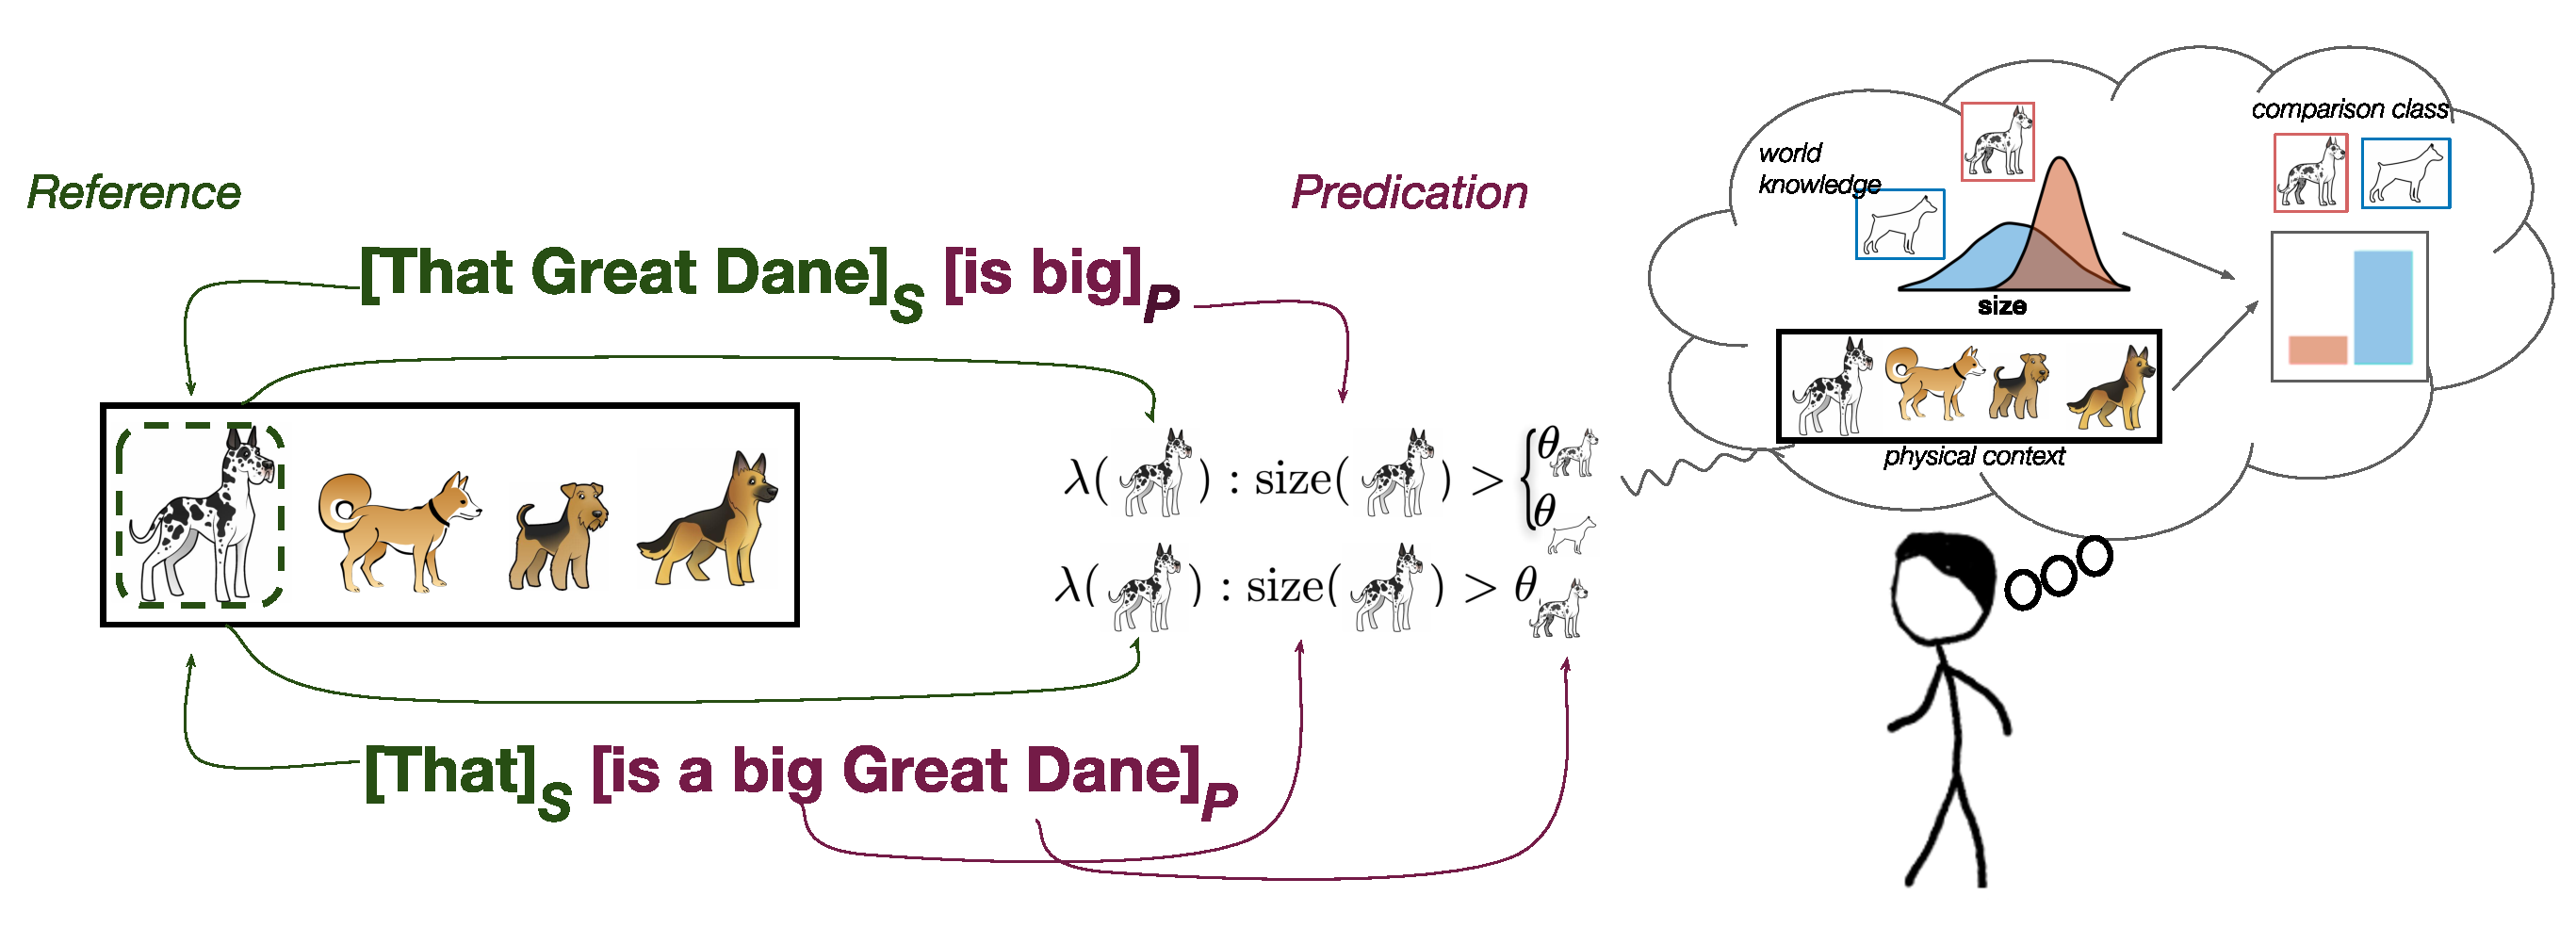
\includegraphics[width=0.9\linewidth]{ref-pred-cartoon-w-subscripts2.pdf}
	\end{center}
	\caption{Cartoon of the inferential account for comparison class determination. The noun (Great Dane) in a sentence can be employed either for the goal of reference (green) or predication (purple), shown in the case when this distinction is made via the syntactic position of the noun (subject S~vs.~predicate P). When the noun is used for reference (top), a listener is left with uncertainty about what to use as the comparison class (dogs or Great Danes) and integrates their world knowledge and the physical context to make this inference.  When the noun is used for predication (bottom), the listener should have less uncertainty about the comparison class: The comparison class is stipulated by the noun.}
	\label{model-cartoon}
\end{figure*}
 
Hence, the utility of the noun as constraining the comparison class is the result of a trade-off between its utility in reference and predication, such that comparison class inference is guided by integrating syntactic with other contextual cues.

\section{Understanding Reference and Predication}
\label{3.1.}
This reference-predication trade-off hypothesis focuses on two basic informational goals, reference and predication, which have been discussed in a great deal of work in semantics, pragmatics and philosophy of language \parencite{michaelson2019, Reboul2001}.
 
\textcite{searle1969speech} conceptualizes both reference and predication as particular kinds of propositional acts, defining conditions to be fulfilled in order to accomplish them. Of particular importance for accomplishing reference is that the expression intended for reference isolates the target referent for the listener \parencite{searle1969speech}. Studies have shown that speakers are aware of this requirement, and being sensitive to contextual variability, adjust the informativity of their referential expression correspondingly, such that this requirement is satisfied \parencite[e.g.,][]{graf2016animal}. In particular, definite descriptions which prenominal adjectives might be a part of have been the focus of a lot of work on reference, converging on the claim that a singular determiner phrase of the form \emph{the $\phi$} triggers two presuppositions: the \textit{existence} presupposition (i.e., that there is an object satisfying the description $\phi$), and the \textit{uniqueness} presupposition (i.e., that such an object is uniquely identifiable) \parencite{syrett2010meaning, michaelson2019}. These same presuppositions generally also hold for pronouns and demonstratives, but do not for indefinite descriptions of the form \textit{a $\phi$} \parencite{braun2017, Reboul2001}. Therefore, our experimental operationalization focusing on predication employs gradable adjectives in indefinite descriptions (s. section \ref{3.2.})

The goal of predication builds upon reference, in that one of the requirements for accomplishing predication is that the same sentence contains a reference to the intended target of predication \parencite{searle1969speech, Reboul2001}. Specifically for relative adjectives, predication is tantamount to communicating a particular property degree, and therefore supplying a felicitous comparison class, for the referent under discussion. Accomplishment of the goal of predication is often roughly equated with the syntactic predicate, which notably might consist of a bare predicative gradable adjective, introduced with a copula. Therefore, one might hypothesize that the noun cannot be the only cue to the comparison class, since predication might be accomplished by a bare adjective.

This review does not attempt to resolve the debate on how exaclty reference and predication might be accomplished. But of particular importance for this work is the flexibility of nouns with respect to both informational goals: combining with the deictic ‘that’, the noun can accomplish reference; but being part of a non-referential expression (e.g., an indefinite description), the noun can contribute to predication \parencite{Reboul2001}. 

The focus of this work are these two relatively basic informational goals, but clearly there are other communicative uses of adjectives. For example, \textcite{barker2002dynamics} distinguishes between \textit{descriptive} and \textit{meta-linguistic} uses of vague adjectives. The former refers to what so far has been considered \emph{predication} applied to relative adjectives, while the latter refers to giving 'guidance concerning what the prevailing relevant standard' of comparison is for the adjective under discussion \parencite[p. 2]{barker2002dynamics}. That is, the goal in this case is to teach the appropriate use of the vague adjective, given a particular property value in context. Another related goal of adjective use might be conveying a subjective opinion about a property \parencite{kaiser2020}. Interestingly, gradable adjectives have been shown to differ in the degree of subjective content they might convey \parencite{scontras2017subjectivity}. Further investigation of these communicative goals and their relation to reference and predication is left open to future research.

The discussed properties of reference and predication lead to the particular experimental operationalisation of the reference-predication trade-off hypothesis, described in the next section. 

\section{Experimental Operationalization}
\label{3.2.}
In present studies, the flexibility of nouns to contribute to either informational goal leads to the operationalization of the reference-predication trade-off hypothesis via a syntactic manipulation, wherein the noun (N) which combines with the gradable adjective (ADJ) appears either in the subject or in the predicate of a sentence. Experiments 1-3 employ sentences including only one critical noun N \parencite{tessler2020}:
\begin{quotation}
	\textit{Subject N}: That N is ADJ. 
	
	\textit{Predicate N}: That's a ADJ N.
\end{quotation}
Experiment 4 focuses on the critical noun N1 syntactically modified by the adjective, which then appears either in the subject or in the predicate of an utterance: 
\begin{quotation}
	\textit{Subject N}: That ADJ N1 is a N2. 
	 
	\textit{Predicate N}: That N2 is a ADJ N1.
\end{quotation} 
Given the referential presupposition of the deictic 'that', subject nouns should be taken as establishing reference.  For the predicate noun condition, reference should be taken as being established by the bare deictic or the second noun N2, respectively. Given the presuppositional nature of definite descriptions, the predicate N conditions were chosen to include an indefinite description, such that the predicate may apply to several members in context and referential pressure be shifted to the subject of the utterance. Furthermore, in the experimental set-up the referent described by critical sentences was perceptually salient, and the task did not involve direct reference resolution, such that referential pressure was generally lower than in experiments described in section \ref{2.4.}.
\pt{discuss in chapter 6 that deconfounding definiteness from syntactic manipulation should be addresses in future research; keep it maximally symmetric in E1-3; tentative predictions for E4: same distinction for "A prize-winner is a big great dane" vs "A big great dane is a prize-winner"; infelicitous presuppositions for both parts being definite; also discuss connection to plural / generics / predagogical language;}

The critical question addressed by this manipulation is how speakers and listeners treat these syntactic frames, asserting the ADJ of referents for whom they are felicitous given one comparison class, but not another (e.g., a \emph{normal-sized} Great Dane can felicitously be described as ‘big’ given the comparison class ‘dogs’, but not ‘Great Danes’). 

The reference-predication trade-off hypothesis predicts that nouns that are more likely to establish reference are less likely to constrain the comparison class. Therefore, when the noun appears in the subject of the utterance, it can be explained away as establishing reference, and hence is a weaker cue towards the comparison class, leaving it open to influences of world knowledge and perceptual context. 

 Conversely, when the noun is taken to contribute to predication, i.e., when it appears in the predicate of the sentence, it is more likely to constrain the comparison class. Therefore, this noun is rather expected to be consistent with the comparison class felicitous in order to describe a target: for instance, the basic-level category label would be more appropriate for setting the comparison class when describing a normal-sized Great Dane as ‘big’ than the subordinate category label. That is, the utterance 'That's a big dog' would be more appropriate than 'That's a big Great Dane' in order to describe a normal-sized Great Dane, because the subordinate category \emph{Great Danes} is generally a large-subordinate category compared to the basic-level category \emph{dogs}, but normal-sized representatives are not necessarily large compared to their subordinate category. 

Note that although the differences in comparison class restriction are approached through the lense of this syntactic manipulation, the underlying communicative goals are the primary driving force in comparison class inference, to which the syntax is just a cue. 
There might well be other syntactic realisations of these informational goals (Reboul, 2001): The sentence “What is big is that Great Dane” seems appropriate in a context where generally big things are discussed; in this utterance reference is accomplished from the predicate, and because of this referential pressure, under the trade-off hypothesis the noun would not be expected to constrain the comparison class, although it appears in the predicate, supporting the view that the syntactic position of the noun is dissociable from the intended communicative goals.

To show that informational goals are primary for comparison class inference as opposed to specific syntactic properties of the adjectival phrase, experiment 4 focuses on manipulating the informational goal the noun is a cue to, while it is directly syntactically modified by the adjective. This manipulation allows to disentangle the effect of the noun position from the effect of syntactic modification of the noun, which are confounded in experiments 1-3. For example, critical sentences in experiment 4 are “That big Great Dane is a prize-winner” (subject-N) or “That prize-winner is a big Great Dane” (predicate-N). The trade-off hypothesis predicts that even directly modified nouns in the subject position contribute to reference, and thus should be less likely to constrain the comparison class, compared to nouns appearing in the predicate.

The next chapter presents results of four behavioural experiments exploring the reference-predication trade-off hypothesis, specifically investigating the use of the size adjectives ‘big’ and ‘small’. These two adjectives are chosen for practical reasons: size is a visually accessible feature, allowing for easy presentation and manipulation of the context in web-based experiments. Furthermore, humans usually have strong expectations about typical size distributions of different natural categories, from which the target referents were sampled for the experiments. Three distinct dependent measures were used to assess the influence of various cues on comparison class inference. This experimental data provides a comprehensive overview of pragmatic and syntactic effects on comparsion class inference. 

\chapter{Experiments}
\label{chapter04}
The reference-predication trade-off hypothesis was tested in four preregistered behavioural web-based experiments employing different dependent measures (Table~\ref{expts-overview}). The crucial manipulation in all experiments was the varying position of the critical noun --- it appeared either in the subject (e.g., “That N is ADJ” or “That ADJ N1 is N2”) or in the predicate (“That’s a ADJ N” or “That N2 is a ADJ N1”) of the sentences presented in the experiments. These sentences described a depicted object which appeared in visual context. 

\begin{table}[t]
	\begin{center}
		\caption{Overview of experiments 1-4.}
		\label{expts-overview}
		\vskip 0.12in
		\fontsize{10}{11}\selectfont
		\setlength{\extrarowheight}{.5em}
		\begin{tabularx}{\textwidth}{>{\hsize=.6\hsize}X>{\hsize=1.1\hsize}X>{\hsize=1.1\hsize}X>{\hsize=1.1\hsize}X>{\hsize=1.1\hsize}X}
			\hline
			& E1:~Syntax \newline Rating & E2:~Noun \newline Production & E3:~Comparison Class Inference & E4:~Direct \newline Modification \\
			\hline
			Research \newline Question & Given two sentences with Ns in different positions, do participants prefer one syntactic frame over the other, depending on the N? & Do speakers produce different Ns given different syntactic frames? & Do listeners infer different comparison classes given different syntactic frames, Ns and contexts? & Is there an effect of syntax on directly modified nouns? \\
			\hline
			Participants & 80 & 190 & 200 & 53 \\
			\hline 
			Task & Slider \newline rating & Fill-in noun & Paraphrase \newline comparison class & Paraphrase \newline comparison class \\
			\hline 
		\end{tabularx}
	\end{center}
\end{table}

These objects were sampled from five different \textit{basic-level} categories: dogs, birds, flowers, trees and fish \parencite{rosch1976}. Within each basic-level category, at least two \textit{subordinate} categories were chosen which exhibit a rather high or rather low amount of the feature described by the gradable adjectives under investigation --- that is, those subordinate categories which people expect to be rather large or rather small representatives of their basic-level categories (s.~Table \ref{tab:stimuli}). For example, for the \textit{dog}-category, the large-subordinate category \textit{Great Danes} and the small-subordinate category \textit{pugs} were chosen. As shown by \textcite{tessler2017warm}, when encountering representatives of such categories described by the adjective consistent with participants’ prior expectations about the degree of the feature-under-discussion, people are a priori more likely to infer the basic-level comparison class than the subordinate comparison class. For example, when encountering the sentence “It’s big” said of a Great Dane (a large-subordinate category for the basic-level category dogs), humans are more likely to infer that the Great Dane is big relative to other dogs in general, than big relative to other Great Danes.  
Following the design of \textcite{tessler2017warm} in these experiments allows to test the effect of syntactic position of the noun on how strong the noun is taken to constrain the comparison class: The reference-predication trade-off hypothesis predicts that nouns in the predicate position constrain the comparison class more strongly than in the subject position, such that a priori using the basic-level noun in predicate position is more felicitous in order to describe a normal-sized large-subordinate object (e.g., a Great Dane) than using a subordinate-label of the object in predicate position. Both nouns would be felicitous in the subject position. Furthermore, encountering a subordinate label in the predicate position, should signal a more extreme feature value than the basic-level label.
\begin{table}[t]
		\begin{center}
			\caption{Experimental items: each basic-level context had two potential targets from an either saliently small or saliently big subordinate category within the basic-level class. Items marked with * were used only in Expt.~2, items marked with $^{+}$ were used in all experiments including Expt.~4.}
			\label{tab:stimuli}
			\vskip 0.12in
			\fontsize{10}{11}\selectfont
			\setlength{\extrarowheight}{.5em}
			\begin{tabularx}{\textwidth}{XXX}
				\hline
				Basic-level category & Smaller referent & Bigger referent\\
				\hline
				Dogs$^+$ & Pug$^+$ & Great Dane$^+$ \\
				Dogs$^+$ & Chihuahua$^+$ & Doberman$^+$\\
				Birds$^+$ & Hummingbird$^+$ & Eagle$^+$  \\
				Fish & Goldfish & Swordfish \\
				Flowers$^+$ & Dandelion$^+$ & Sunflower$^+$\\
				Trees$^+$ & Bonsai$^+$ & Redwood$^+$\\
				Birds* & Sparrow* & Goose* \\
				Birds* & Canary* & Swan* \\
				Fish* & Clownfish* & Tuna* \\
				Flowers* & Daisy* & Peony* \\
				\hline     
			\end{tabularx}
		\end{center}
\end{table}
Therefore, in all experiments, the referents were described by the adjective matching prior feature-degree expectations; for instance, Great Danes and sunflowers were always described as \textit{big}, and pugs or daisies as \textit{small}. 

The structure of all experiments was similar. First, participants completed a bot-check trial (Fig.~\ref{captcha}): Participants read a sentence where a named speaker asked a named listener: “It’s a beautiful day, isn’t it?”. The speaker and listener names were sampled from lists of ten popular male and female English names (s. Appendix \ref{appendix}). For example, the sentences read: “James says to Linda: 'It’s a beautiful day, isn’t?'; Who is James talking to?”.  Participants were asked to fill-in in lowercase who the listener is talking to. Participants were provided feedback and had maximally three attempts to fill-in the correct name. They were only allowed to proceed, if they successfully completed the bot check. Then, participants read instructions and completed practice trials, before completing main trials. After the main trials, they completed a socio-demographic post-test questionnaire, where they were asked to indicate their native language and optionally provide further information. 
For all experiments, participants were recruited via the crowd-sourcing platform Amazon’s Mechanical Turk; only participants with IP addresses in the United States and work approval rating of at least 95\% were permitted to participate. Participants were restrained from taking part in multiple experiments of this series.  

The first experiment (E1, Sentence Rating Experiment) was a sentence rating experiment, wherein participants had to rate two sentences which differed in the position of the noun (subject-N~vs.~predicate N) and the specificity of the noun (basic-level~vs.~subordinate label), as describing an object in context. 
In the second experiment (E2, Noun Production Experiment), participants had to fill-in the missing noun of a sentence describing the size of a referent in context. The position of the missing noun was varied. 
In the third experiment (E3, Comparison Class Inference Experiment), participants provided the inferred comparison classes via a free-production paraphrase, given sentences which varied by the noun category and its position, as describing a referent in different contexts. 
Finally, the fourth experiment (E4, Direct Modification Experiment) gathered inferred comparison classes in a paradigm akin to E3, but from sentences wherein the critical subordinate noun appearing in subject or predicate position was always syntactically modified by the adjective. 
All experimental materials and data can be found under \texttt{https://github.com/polina-tsvilodub/bSc-thesis}. All experiments were realized using the \_magpie-framework \parencite{magpie}. 
All experiments and preregistrations can be viewed under \texttt{https://tinyurl.com/y2b7ajg7}. %\pt{preliminary link}
\begin{figure*}[t]
	\begin{center}
		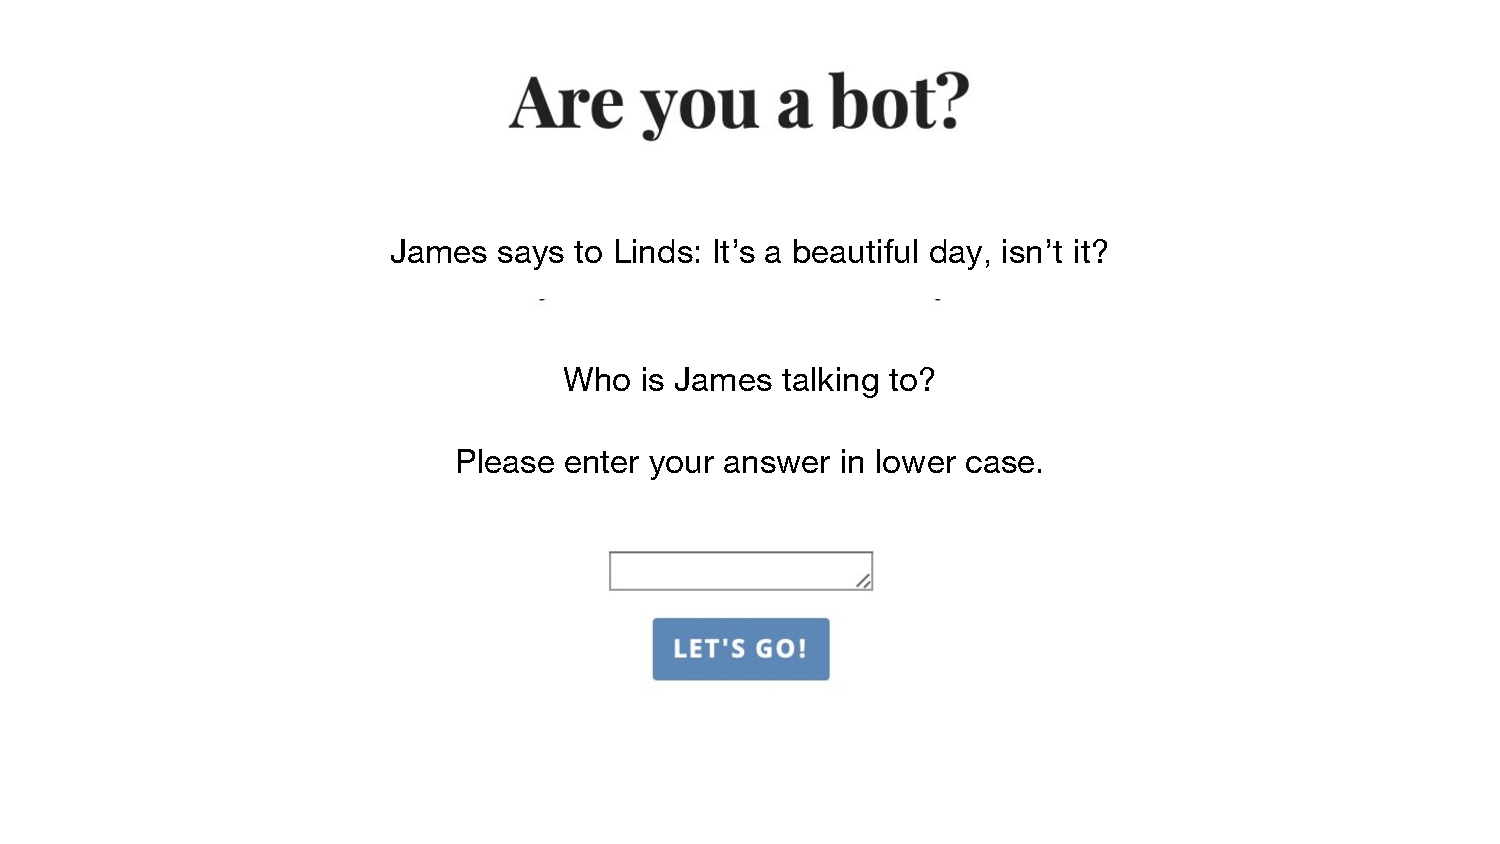
\includegraphics[width=\linewidth]{screenshots/captcha.pdf}
	\end{center}
	\vspace{-1.5cm}
	\caption{Example view of the bot check trial: The speaker James addresses the listener Linda.}
	\label{captcha}
\end{figure*}

\section{Experiment 1: Sentence Rating Experiment}

The aim of the sentence rating experiment was to investigate whether participants prefer one syntactic frame over the other, given two truth-conditionally equivalent sentences with different noun positions, depending on the noun category. The type of the noun and its syntactic position differed within-subjects.

\begin{figure*}[t]
	\begin{center}
	%	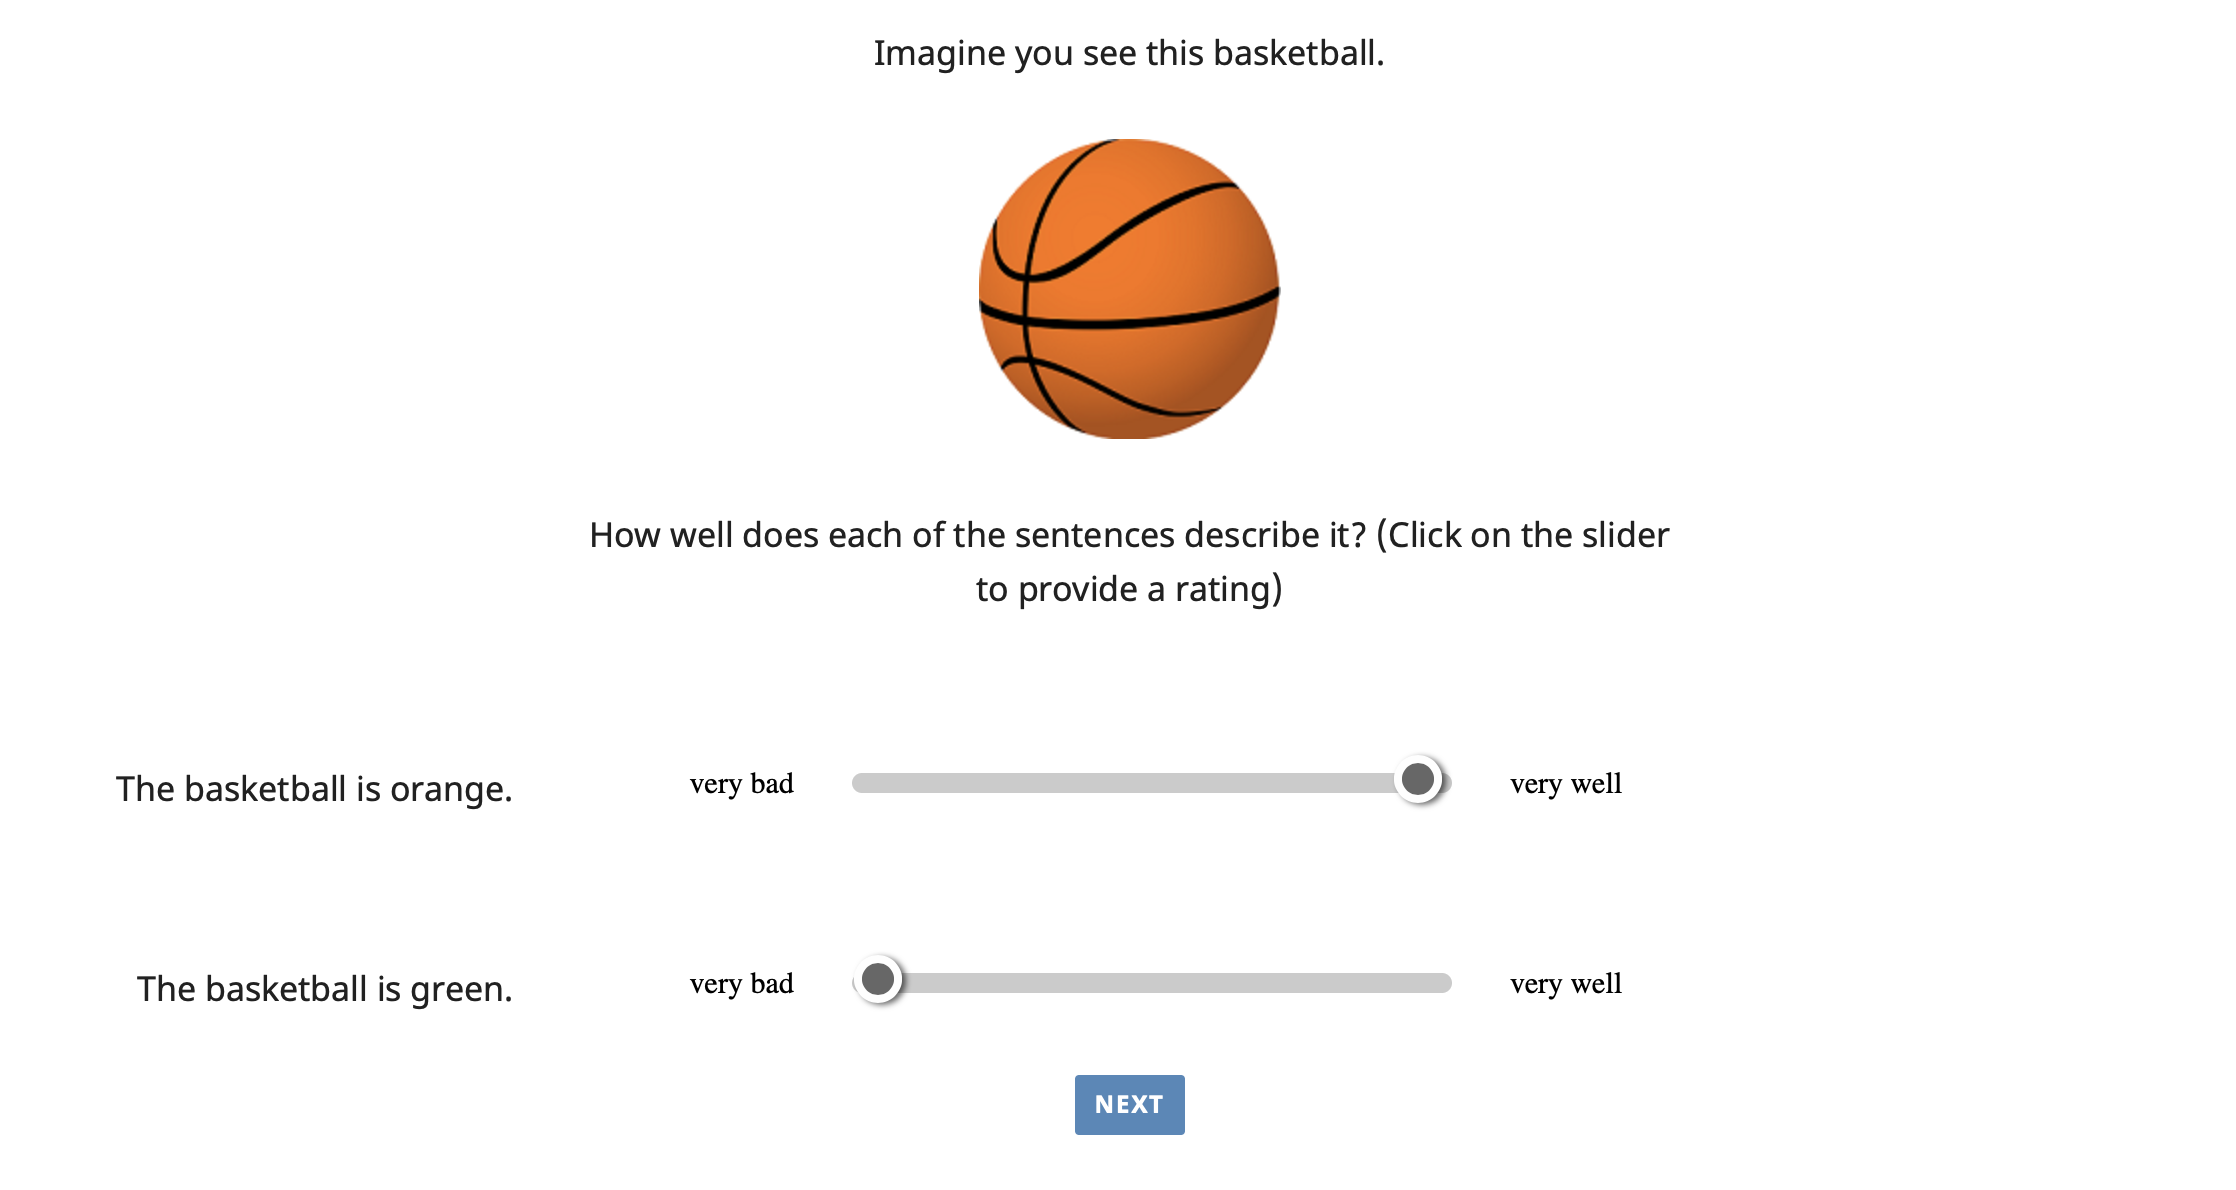
\includegraphics[width=0.7\linewidth]{warmup_basketball.png}
		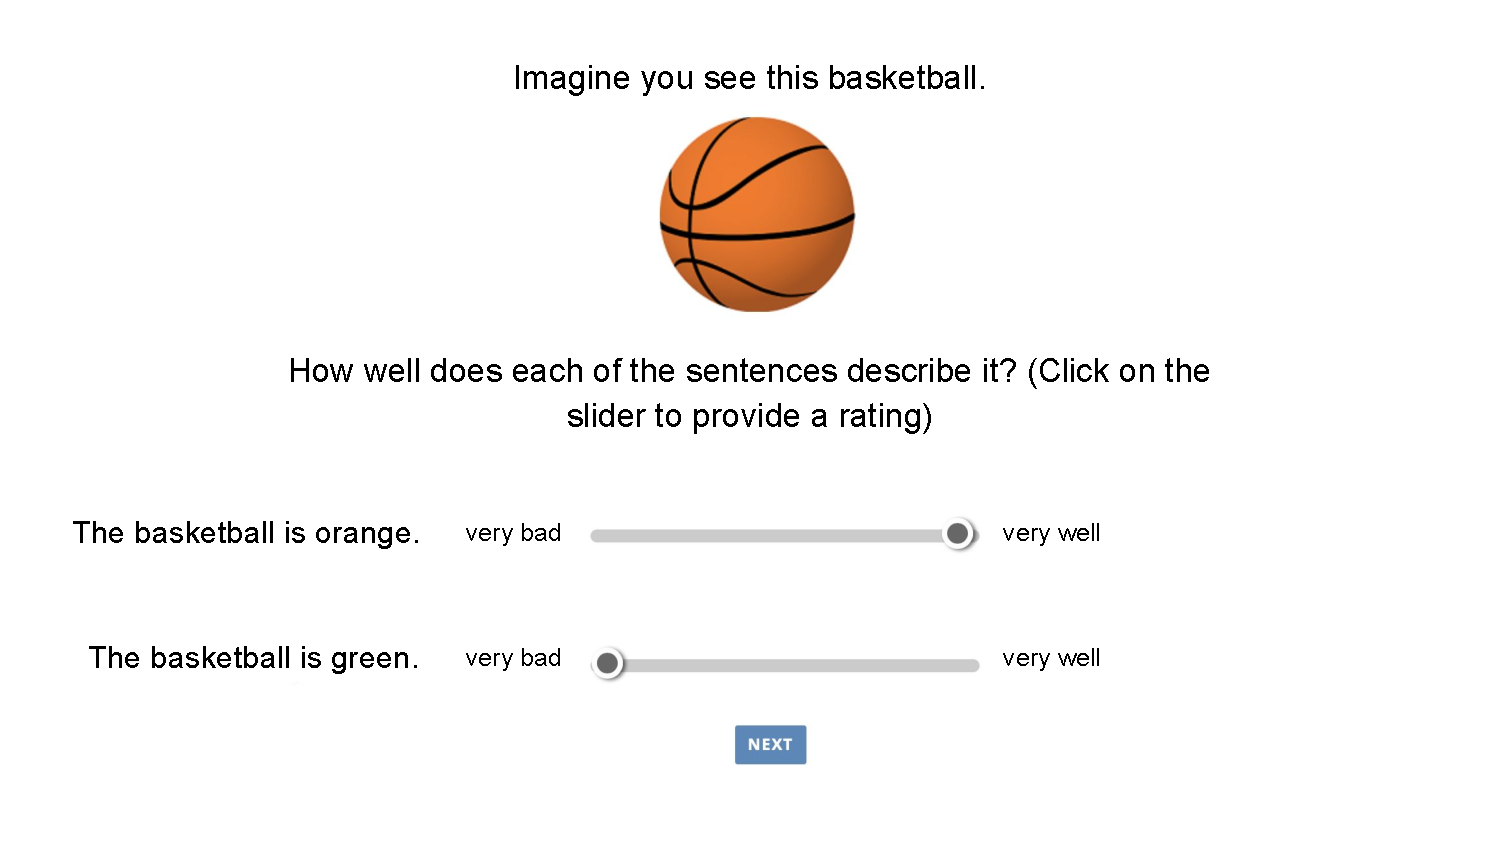
\includegraphics[width=\linewidth]{screenshots/basketball.pdf}
	\end{center}
	\vspace{-1cm}
	\caption{Example view of the sentence rating warm-up trial wherein participants rated sentences about the depicted basketball. }
	\label{warmup-basketball}
\end{figure*}
First, participants completed two warm-up trials to familiarize themselves with the slider rating procedure (Fig.~\ref{warmup-basketball}). On one trial, participants read: “Imagine you see this basketball” above a picture of an orange basketball, and read below the question: “How well does each of the sentences describe it? (Please click on the slider to provide a rating)”. Two sentences appeared below: “The basketball is orange” and “The basketball is green”, to be rated on sliders ranging from “very bad” to “very well”. In the background, the ratings were mapped onto a scale ranging from 0 to 100. The slider was light gray, with a round handle appearing upon clicking on the slider track. The same sliders were used in the main trials. On the other warm-up trial, participants read: “Imagine you see this chair” above a picture of a purple chair. The sentences to be rated appearing below were: “The chair is yellow”, and “The chair is blue”. The order of the warm-up trials was randomized.    

\begin{figure*}[t]
	\begin{center}
		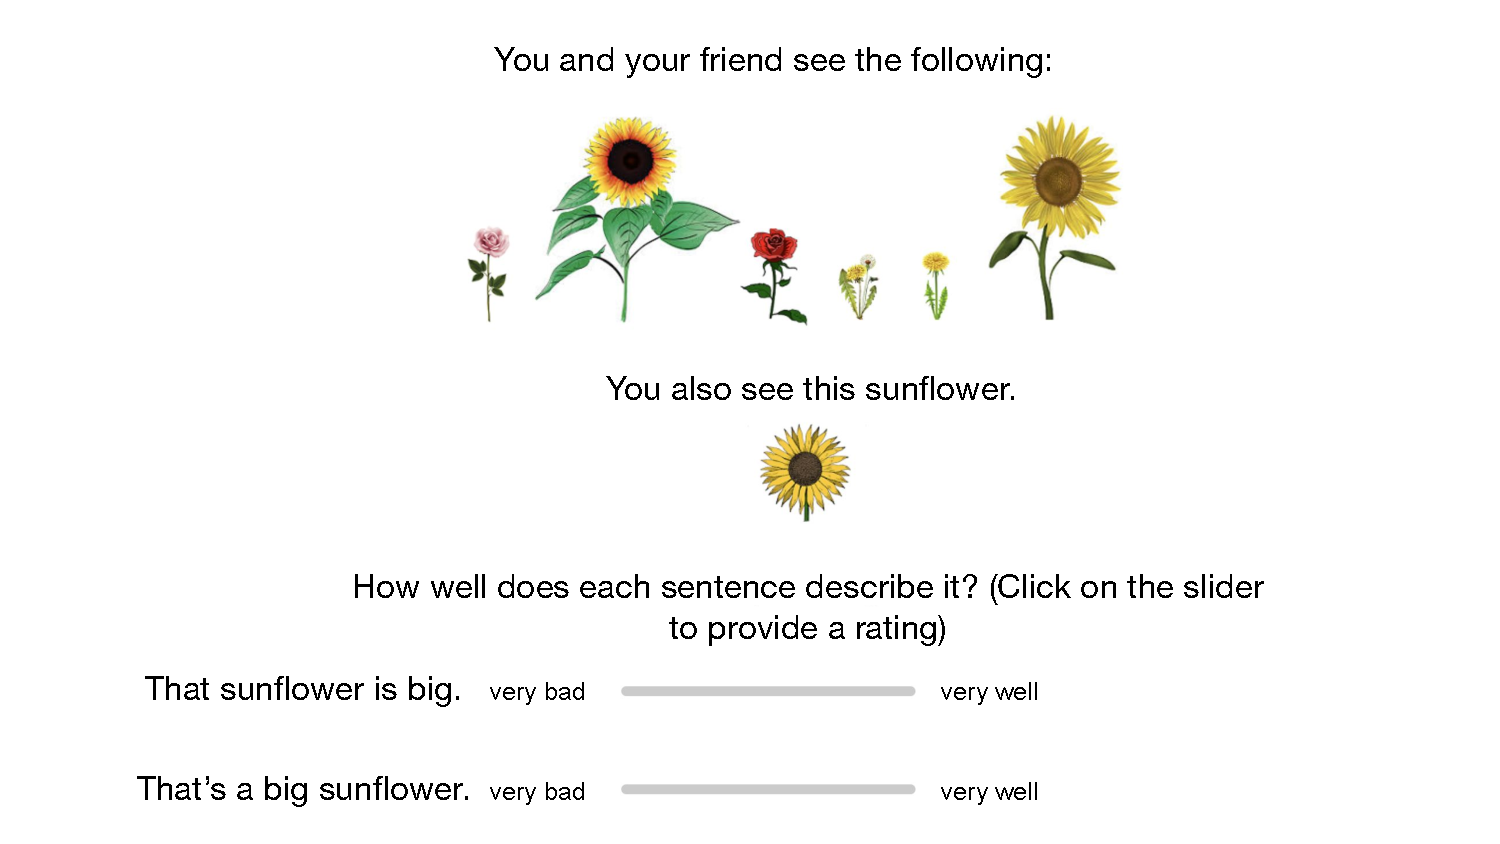
\includegraphics[width=\linewidth]{screenshots/main_rating_subN_big.pdf}
	\end{center}
	\vspace{-0.5cm}
	\caption{Example view of a sentence rating main trial: The critical noun is a subordinate target label of a large-subordinate category, appearing in the subject or predicate of the sentence.}
	\label{rating-main}
\end{figure*}
Then, participants completed six main trials (Fig.~\ref{rating-main}). Participants read “You and your friend see the following:” above a basic-level context picture (e.g., a group of flowers). In all experiments, the basic-level context pictures consisted of six members of the same basic-level category as the referent of the trial, including two other members of the same subordinate category as the referent, and four other objects. The six members consisted of two members of a large-subordinate, a medium-sized subordinate, and a small-subordinate category within the basic-level category each (e.g., the flower-context consisted of two sunflowers, two roses and two dandelions; s.~Fig.~\ref{rating-main}). The context was used to set the overall reference comparison class for the targets. It also set the visual reference frame.
Below, they read the sentence “You also see this SUB\_N”, where SUB\_N was the subordinate label of the target referent, which appeared depicted below, such that participants knew the subordinate category of the referent. The pictures depicted referents a little smaller than members of the same subordinate category in the context, such that the felicitous comparison class was pushed towards the basic-level category of the target.
Below, the question about the critical sentences appeared: “How well does each of the sentences describe it? (Click on the slider to provide a rating)”. Then, the two critical sentences appeared left of the sliders one below the other. The sliders ranged from “very bad” to “very well”. On every trial, in one of the sentences the noun appeared in the subject (e.g. “That N is \{big/small\}”), in the other in predicate position (“That’s a \{big/small\} N”). The order in which these syntactic conditions appeared was randomized between-subjects. 
On half of the trials, the noun was the basic-level target label (e.g., dog); on the other half it was the subordinate target label (e.g., Great Danes), balanced within-subjects. 
Participants saw each of the six possible contexts once, and for each context, one of the two possible targets (large-subordinate vs. small-subordinate category representative) was sampled, balanced within-participants (Table \ref{tab:stimuli}). 

The reference-predication trade-off hypothesis predicts that the effect of syntax on the rating will be more pronounced for sentences containing a subordinate noun than for sentences constaining a basic-level noun because a subordinate noun in predicate position would communicate an infelicitous comparison class for a normal-sized referent, while a basic-level predicate would be felicitous. That is, sentences with a basic-level noun in the predicate position are expected to receive a higher rating than sentences with a subordinate noun in the predicate, but a smaller difference in the ratings is expected for sentences with a noun in the subject position because either noun type can be felicitously used to pick out the referent. Given the specification of the statistical model (s.~Section~\ref{rating-results-section}), this prediction would be evidenced by a a negative credible estimate of the noun $\times$ syntax interaction.   

\subsection{Participants}
\rlgetvariable{myvars-rating.csv}{nSubj} participants were recruited and \rlgetvariable{myvars-rating.csv}{nExcludedTotal} were excluded for indicating a native language other than English, failing the practice trials or providing the same responses on every trial (see Appendix \ref{appendix}). The experiment took about 5 minutes and participants were compensated \$0.80. If partial data was missing from a participant, available data was used for analyses. 
\subsection{Results}
\label{rating-results-section}
For all reported experiments, maximal random effects structure licensed by the design was used \parencite{barr2013}. All statistical analyses were performed using the language R, in particular using the package \texttt{brms} for computing Bayesian regression models \parencite{Rteam2013, burkner2017advanced}.

A Bayesian linear mixed-effects regression model was fit for this experiment, predicting the sentence rating from the syntactic condition of the sentence (subject~vs.~predicate N), the noun type (basic-level~vs.~subordinate target label), their interaction and by-participant and by-target random intercepts and random slope effects of syntax, noun type and their interaction.\footnote{Model in \texttt{brm}-style syntax: \texttt{rating $\sim$ syntax * NP + (1 + syntax*NP | subject) + (1 + syntax*NP | target)}} 
Both predictors were sum-coded, coding both the subject-noun and the basic-level noun conditions as 1 and the other levels as -1, respectively. Default priors were used.
An exploratory model including a main effect of syntactic condition order was also fit, revealing no effect of syntactic condition order, so the data was collapsed across the two conditions for further analyses. 

\begin{figure*}[t]
	\begin{center}
		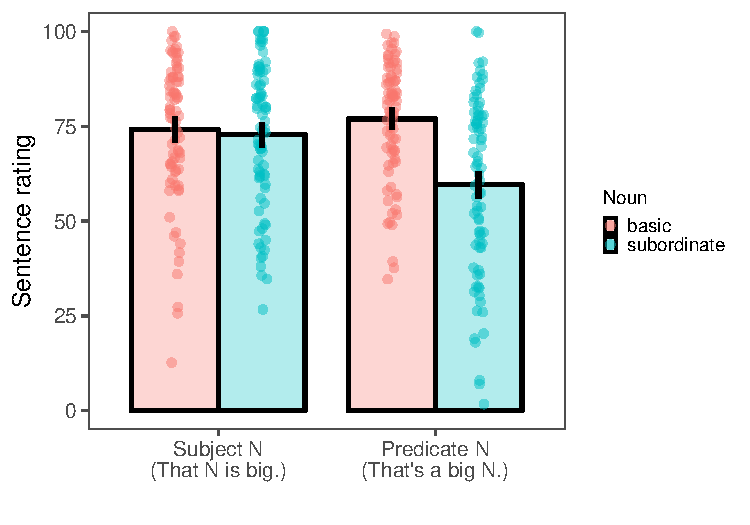
\includegraphics[width=0.7\linewidth]{expt-syntax-rating-prereg-bars-revised.pdf}
	\end{center}
 	\vspace{-0.3cm}
	\caption{Experiment 1 results: Mean ratings for how well sentences which differed in the syntactic position of the noun (x-axis)  and the noun-label (color) described a typically-sized referent (e.g., a Great Dane) in basic-level context.  Points represent participant means within condition. Error-bars denote bootstrapped 95\% confidence intervals (bootstrapping independent of random-effects structure).}
	\label{rating-results}
\end{figure*}
Consistent with predictions, participants substantially dispreferred sentences with a subordinate noun in the predicate compared to the subordinate position, but no effect of syntax was found for the basic-level nouns, as indicated by the syntax $\times$ noun-type interaction ($\beta = \rlgetnum{expt1_brm.csv}{Rowname}{syntax:NP}{Estimate}{2}  [\rlgetnum{expt1_brm.csv}{Rowname}{syntax:NP}{l.95..CI}{2}, \rlgetnum{expt1_brm.csv}{Rowname}{syntax:NP}{u.95..CI}{2}]$) (Fig.~\ref{rating-results}).\footnote{All results report the mean and 95-\% Bayesian credible interval} 
Additionally, an overall preference for basic-level nouns ($\beta = \rlgetnum{expt1_brm.csv}{Rowname}{NP}{Estimate}{2} [\rlgetnum{expt1_brm.csv}{Rowname}{NP}{l.95..CI}{2},\rlgetnum{expt1_brm.csv}{Rowname}{NP}{u.95..CI}{2}] $) and the subject-noun syntactic structure ($\beta = \rlgetnum{expt1_brm.csv}{Rowname}{syntax}{Estimate}{2} [\rlgetnum{expt1_brm.csv}{Rowname}{syntax}{l.95..CI}{2}, \rlgetnum{expt1_brm.csv}{Rowname}{syntax}{u.95..CI}{2}] $) was found. Furthermore, a relatively high by-target variance revealed that some items received overall lower ratings, possibly due to differing namability or typicality of the items (by-target intercept: $\beta = \rlgetnum{expt1_random_brm.csv}{Rowname}{sd(Intercept)}{item.Estimate}{2} [\rlgetnum{expt1_random_brm.csv}{Rowname}{sd(Intercept)}{item.l.95..CI}{2}, \rlgetnum{expt1_random_brm.csv}{Rowname}{sd(Intercept)}{item.u.95..CI}{2}]$). A relatively high by-participant variation indicated differences in overall rating preferences (by-subject intercept:~$\beta = \rlgetnum{expt1_random_brm.csv}{Rowname}{sd(Intercept)}{submission_id.Estimate}{2} [\rlgetnum{expt1_random_brm.csv}{Rowname}{sd(Intercept)}{submission_id.l.95..CI}{2}, \rlgetnum{expt1_random_brm.csv}{Rowname}{sd(Intercept)}{submission_id.u.95..CI}{2}]$).
Finally, an exploratory analysis including a target size predictor (small-subordinate vs. large-subordinate category) did not reveal any size-effects on the rating. 

To sum up, the sentence rating experiment showed that participants are sensitive to the position and the type of the noun, dispreferring sentences where a noun that provided an a priori less felicitous comparison class appeared predicatively.  

\section{Experiment 2: Noun Production Experiment}    

%classification of responses
%results: main, by-participant / by-item, by-size  

The goal of the noun production experiment was to investigate whether participants produce nouns of different categories in a free-production setting, given different syntactic frames.  The noun slot of the critical sentences in the main trials appeared either in the subject position (i.e., in “That \_\_ is \{big/small\}“) or in the predicate position (i.e., in “That’s a \{big/small\} \_\_”), manipulated between-subjects. 

\begin{figure*}[t]
	\begin{center}
		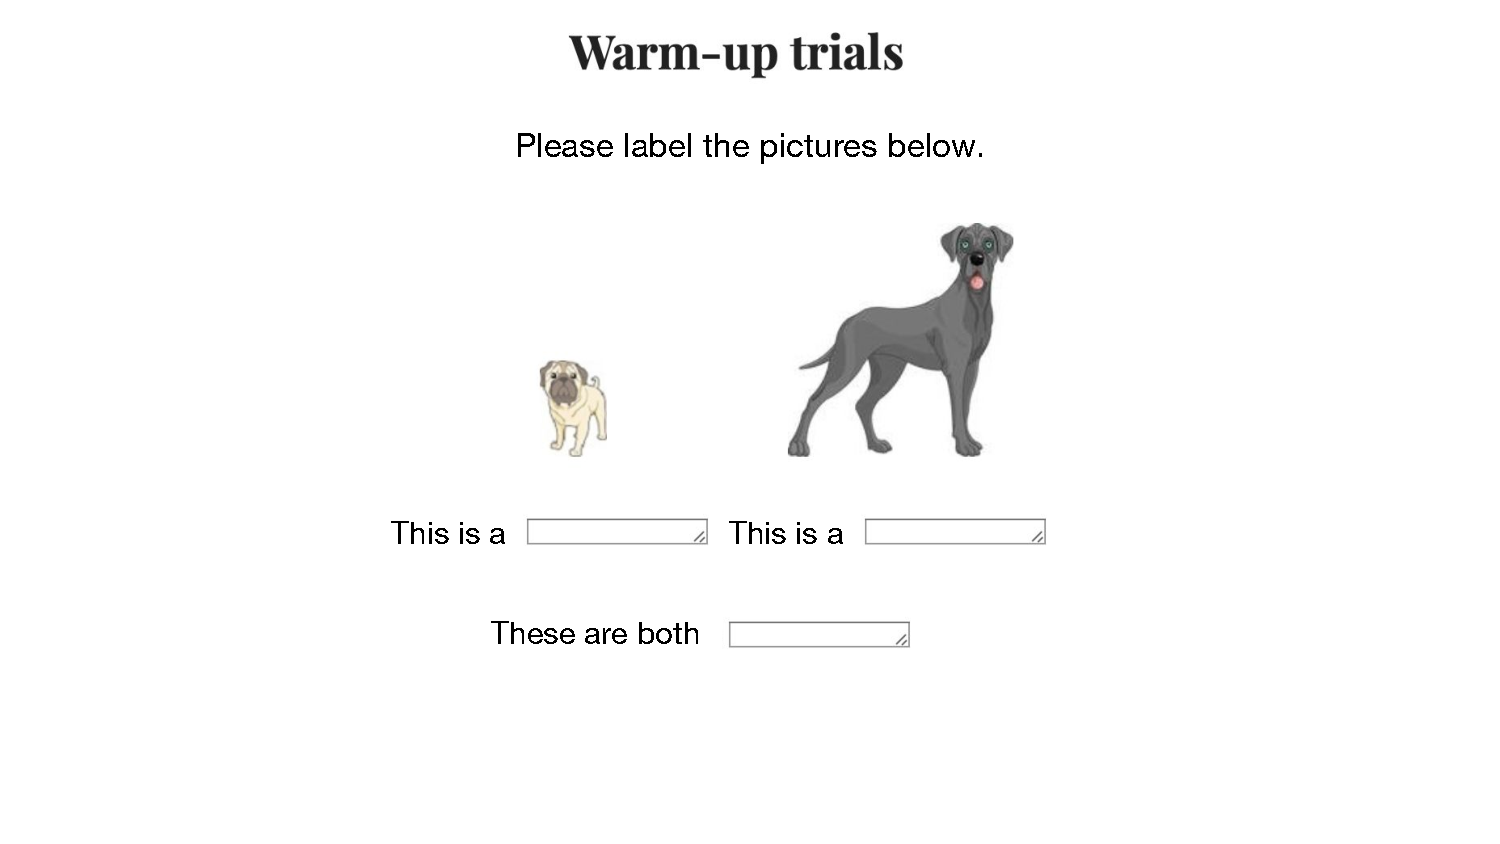
\includegraphics[width=\linewidth]{screenshots/warmup_dogs.pdf}
	\end{center}
	\vspace{-2cm}
	\caption{Example view of the noun production warm-up trial: Participants have to label a large-subordinate (Great Dane, right) and a small-subordinate target (pug, left) for the dogs-category, and provide the common label below.}
	\label{warmup-production}
\end{figure*}
Participants completed two experimental blocks, each consisting of three warm-up trials and three main trials. In the warm-up trials participants familiarized themselves with the subordinate categories used in the main trials. They saw pictures of a member from a large-subordinate and a small-subordinate category within one of the basic-level categories used in the main trials within the same block (e.g., a Great Dane and a pug) (Fig. \ref{warmup-production}). Participants were prompted to provide labels for these pictures. Below they were prompted to provide a common label for both pictures (i.e., dogs), so that they were `warmed-up' to provide lables of different categories. They were provided feedback for the labels and could proceed upon adjusting their labels to correct responses. The number of attempts participants needed until they filled-in the correct labels was recorded. In this experiment, four additional subordinate categories were used, which can be found in Table \ref{tab:stimuli} marked with *. For each participant, six out of ten possible contexts were sampled. Three of these contexts and their corresponding targets appeared in the first experimental block, and the other three in the second. The trial order within the warm-up block and the main block was randomized. 

\begin{figure*}[t]
	\begin{center}
		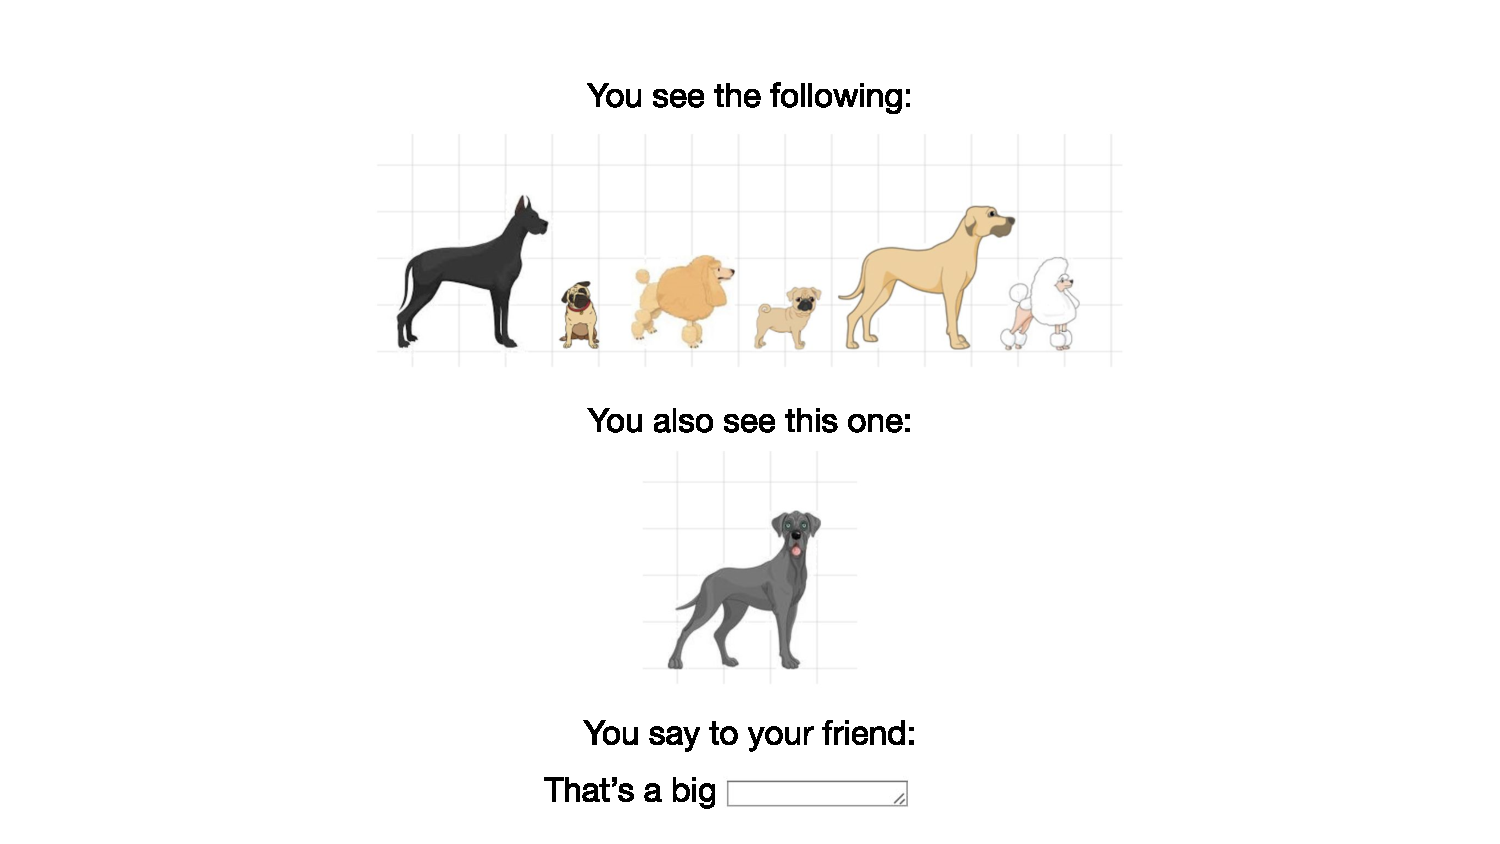
\includegraphics[width=\linewidth]{screenshots/main_prod_predN_big.pdf}
	\end{center}
    \vspace{-0.5cm}
	\caption{Example view of the noun production main trial: Participants fill-in the noun in the predicate position of a sentence describing a large-subordinate target in basic-level dogs context.}
	\label{main-production}
\end{figure*}
On the main trials, participants read: “You see the following:” above a basic-level context picture, akin to the contexts used in Experiment 1. Below, they read “You also see this one:” and saw a picture of the target referent. Then they read: “You say to your friend:”, prompting them to fill-in the missing noun in the sentence: for the subject-noun condition, the template was “That\_\_ is \{big/small\}”, for the predicate-noun condition, the template to be completed was “That’s a \{big/small\} \_\_ “ (Fig. \ref{main-production}).  
The size of the target referent was balanced within-participants: on three trials, participants saw referents from a small-subordinate category, and on three, they saw referents from a large-subordinate category. For each context, participants saw only one of the possible targets (e.g., the large or the small subordinate target).

The reference-predication hypothesis predicts that speakers sensitive to listeners' expectations about accomplishment of communicative goals should be more likely to produce basic-level target labels than subordinate target labels in the predicate compared to the subject position. A positive credible regression coefficient for the effect of syntax would confirm this prediction, indicating a higher proportion of basic-level responses in the predicate compared to the subject position. 

\subsection{Participants}
\rlgetvariable{myvars-np.csv}{nSubj}  participants were recruited, and \rlgetvariable{myvars-np.csv}{nExcludedTotal}  were excluded for indicating a native language other than English or for failing the warm-up trials. The exclusion criterion was taking more than four attempts on any warm-up trial to provide the expected answer upon correction. The experiment took about 7 minutes and participants were compensated \$1.00. If partial data was missing from a participant, available data was used for analyses. 
 
\subsection{Results}
\begin{figure*}[t]
	\begin{center}
		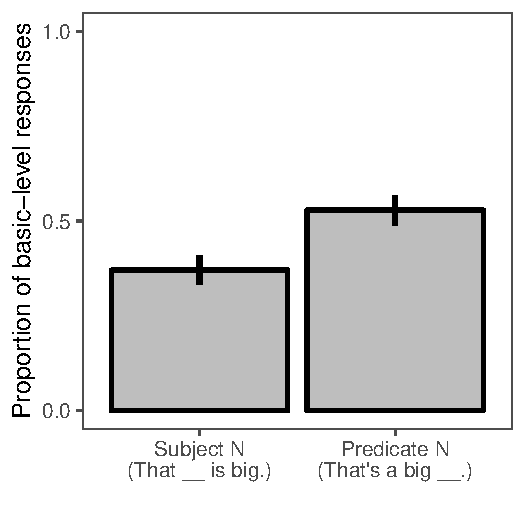
\includegraphics[width=0.5\linewidth]{expt-np-prod-prereg-bars-revised.pdf}
	\end{center}
	\vspace{-0.3cm}
	\caption{Experiment 2 results: Proportions of freely-produced basic-level labels (e.g., \emph{dog}) in different syntactic frames (x-axis) when the referent was a typically-sized member of a subordinate category (e.g., a normal-sized Great Dane). Error-bars denote 95\% bootstrapped confidence intervals.}
	\label{production-results}
\end{figure*}
The responses provided by participants were categorized manually into basic-level or subordinate-level labels of the targets, disregarding the noun number and spelling mistakes. 5 responses were superordinate referent labels (i.e., more general labels like `animals') and were collapsed with basic-level labels. 16 (1.4\%) uncategorizable responses were excluded from analysis. 
A logistic generalized mixed-effects Bayesian regression model was fit, regressing the response category (basic-level~vs.~subordinate target label) against the syntax of the sentence (subject-N~vs.~predicate-N), random by-participant and by-referent intercepts and random by-referent slope effects of syntax.\footnote{In brm-style syntax: \texttt{response\_category $\sim$ syntax + (1 | subject) + (1 + syntax | target)}}
Default priors were used. The predictor was sum-coded, coding predicate-N syntax as 0.5 and subject-N syntax as -0.5.

Consistent with predictions, a strong effect of syntactic position of the noun was found, indicating that participants were more likely to use basic-level labels in the predicate position ($\beta = \rlgetnum{expt2_brm.csv}{Rowname}{syntax_contr}{Estimate}{2} [\rlgetnum{expt2_brm.csv}{Rowname}{syntax_contr}{l.95..CI}{2}, \rlgetnum{expt2_brm.csv}{Rowname}{syntax_contr}{u.95..CI}{2}]$;~Fig.~\ref{production-results}). That is, participants were more likely to provide the noun matching the felicitous comparison class in the predicate position, but more likely to use the noun with higher referential utility in the subject.    
As expected, an exploratory model including a main effect of referent size (large-subordinate vs. small-subordinate category) did not reveal any differences between target types. By-target variation revealed that participants were generally more likely to produce subordinate labels for some targets than for others (by-target intercept: $\beta = \rlgetnum{expt2_random_brm2.csv}{Rowname}{Intercept}{target.Estimate}{2} [\rlgetnum{expt2_random_brm2.csv}{Rowname}{Intercept}{target.l.95..CI}{2}, \rlgetnum{expt2_random_brm2.csv}{Rowname}{Intercept}{target.u.95..CI}{2}]$). For example, participants were very likely to produce the subordinate label for the swan-item, possibly due to namability effects.

The noun production experiment showed that speakers are sensitive to the syntactic structure of the sentence and flexibly adjust their noun choices in order to communicate a felicitous comparison class, when presented with a free-production task.  
 
 
\section{Experiment 3: Comparison Class Inference Experiment}
\label{experiment3}
The two previous experiments support the reference-predication trade-off view, by showing that participants disprefer sentences like “That’s a big Great Dane” in order to describe a normal-sized Great Dane, but accept either target label in the sentence subject. The goal of this comparison class inference experiment was to measure comparison class inferences more directly, presenting participants with sentences they had to paraphrase. The types of inferred comparison classes were investigated, as influenced by the position of the critical noun in the sentence (subject~vs.~predicate), the type of noun (basic-level~vs.~subordinate~vs.~'one') and the visual context of the sentence (basic-level~vs.~subordinate context). All three factors were manipulated within-subjects.

In this experiment, participants first completed a comparison class paraphrase practice trial, akin to the paradigm employed in the main trials. Participants were told that on the main trials they will see a sentence containing a word that is relative, and their task will be to figure out what this word is relative to. They read an example task: “Speaker A: ‘The Empire State building is tall.’ What do you think speaker A meant?”. Below they saw a paraphrase template where they provided the inferred comparison class of the adjective \emph{tall}: “The Empire State building is tall relative to other\_\_” (blank to be completed with the inferred comparison class). Participants were provided feedback on their response and had to correct it to one of the possible options among \{buildings, skyscrapers, houses, constructions\}. 
Then, participants completed two blocks consisting of labeling warm-up trials and main paraphrase trials. Three of the six basic-level categories used in this experiment were sampled for the first block, with the respective subordinate category members appearing in the warm-up trials, the other three categories appeared in the second block (Table \ref{tab:stimuli}). These labeling warm-up trials are of the same kind as in Experiment 2 (Fig. \ref{warmup-production}). 

\begin{figure*}[t]
	\begin{center}
		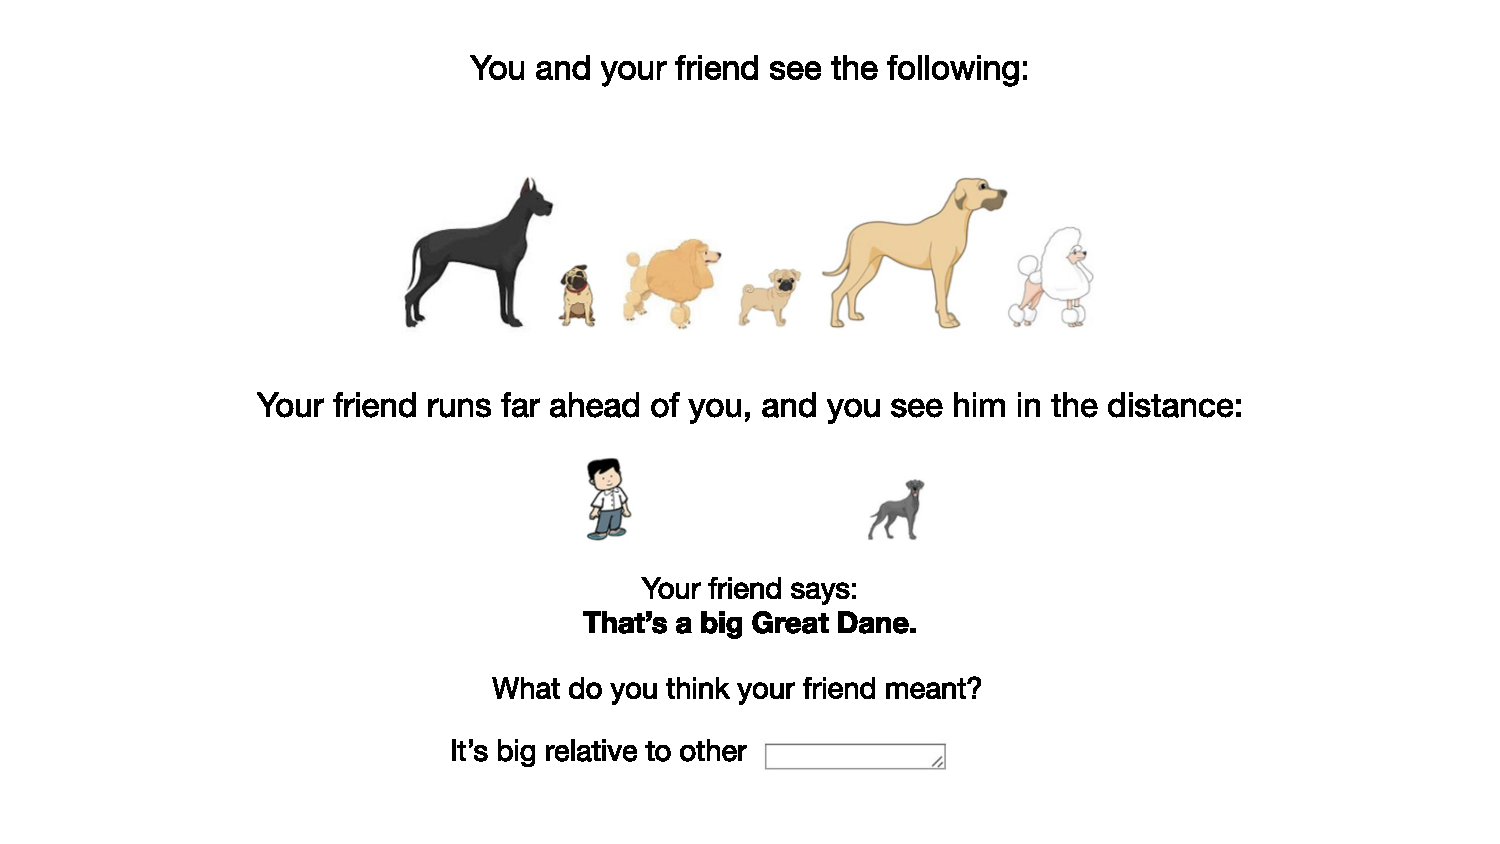
\includegraphics[width=\linewidth]{screenshots/main_cci_basicContext_predSubN_big.pdf}
	\end{center}
	\vspace{-0.5cm}
	\caption{Example view of a comparison class inference main trial: Participants paraphrased the critical utterance with a subordinate noun in predicate position, which appeared in basic-level context, describing a large-subordinate target.}
	\label{main-cci}
\end{figure*}
\begin{figure*}[t]
	\begin{center}
		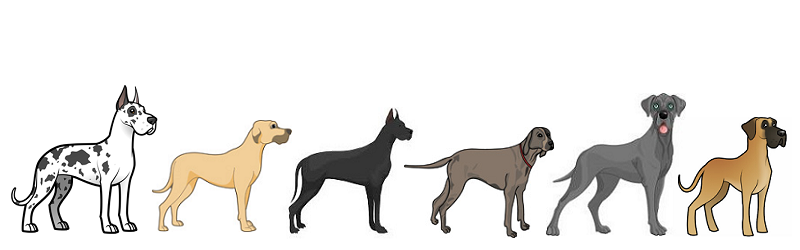
\includegraphics[width=0.7\linewidth]{dog-parade-great-dane-screenshot.png}
	\end{center}
	\caption{Example view of a subordinate context: For the category Great Danes, the context depicts six different Great Danes.}
	\label{cci-sub-context}
\end{figure*}
For the main trials there were basic-level and subordinate-level contexts for each possible referent. Basic-level contexts were identical to the contexts of respective categories in Experiment 1 and Experiment 2 (Figs.~\ref{main-production}, \ref{rating-main}); the subordinate contexts consisted of six other representatives of the same subordinate category as the target referent. For example, the subordinate context for a Great Dane consisted of a picture of a group of six other Great Danes (Fig.~\ref{cci-sub-context}). Within each main trial block, there were six trials, wherein for each of the three sampled categories, one possible referent appeared in the corresponding basic-level context (e.g., for the category dogs, the Great Dane appeared in basic-level dog context), and the other possible referent appeared in the corresponding subordinate context (i.e., then the pug appeared in subordinate pugs-context). 
The referent was described by a critical sentence in which the noun could appear in the subject or in the predicate of the sentence. The noun could be either the basic-level (e.g., dog) or the subordinate label of the referent (e.g., Great Dane). Furthermore, a baseline condition with an anaphoric ‘one’ in the noun position was included, in order to measure the baseline influence of the visual context on comparison class inference: the anaphora is most likely to be resolved contextually, meaning ``dog" in the basic-level context and ``Great Dane" in subordinate context \parencite{goldberg2017one}. Crossing the visual context (basic vs. subordinate), the syntax (subject-N vs. predicate-N) and the possible nouns (basic vs. subordinate vs. ‘one’) results in a 2x2x3 design, yielding 12 unique conditions.\footnote{Due to my coding mistake, the conditions were balanced at the level of individual factors. That is, each participant saw six trials in basic-level and six trials in subordinate context, six trials in the subject and six in the predicate condition, as well as four trials in each noun-condition. However, participants potentially did not see all 12 possible combination of these factors.}
Each participant saw a total of 12 main trials.   

On main trials, participants read “You and your friend see the following:” above a context picture  (Fig. \ref{main-cci}). Below, they read: “Your friend runs far ahead of you, and you see him in the distance:”. The illusion of distance was created contextually in order to disguise the perceptual size of the target referent and push participants towards inferring the size of the referent from the sentence, rather than perceptually, while conveying its subordinate category. This illusion was supported by the picture appearing below, wherein the small target referent was depicted next to a small person (as compared to the context, i.e., appearing in distance). Below, participants read:~“Your friend says:”, followed by the critical sentence. Participants were asked “What do you think your friend meant?”, followed by the paraphrase template “It is \{big/small\} relative to other \_\_”, blank to be completed with the inferred comparison class. The order of context, noun and syntax conditions was randomized for each participant.

When participants don’t have access to visually assessing the size of a referent and need to infer the comparison class from the sentence, they might be more sensitive to linguistic cues like the sentence structure. According to the reference-predication hypothesis, they would be more likely to take the noun as a cue to the comparison class when the noun appears in the predicate of that sentence, than when it appears in the subject. 
When the noun appears in the subject, comparison class inference can be driven by other pragmatic inferences, e.g., by world knowledge and visual context. If this is true, more basic-level comparison classes should be inferred from sentences appearing in basic-level context, compared to subordinate context. A credible positive regression coefficient for the effect of context would support this prediction. Additionally, inferences drawn from the anaphoric 'one' which is the baseline condition for the effects of visual context are then expected to mirror this difference, such that more basic-level comparison class should be inferred in the basic-level context than in the subordinate context, evidenced by a credible positive estimate for the respective contrast (s. Section~\ref{cci-results-text}; \textcite[cf.][]{goldberg2017one}).
 
In particular, nouns with a high referential utility (e.g., subordinate target labels given a basic-level set of distractors, \textcite[cf.][]{graf2016animal}) should highlight the main reference-predication prediction, by providing strong referential cues in the subject, but potentially signalling a comparison class different from prior world knowledge and perceptual context in the predicate. That is, participants are expected to infer more subordinate comparison classes (i.e., less basic-level ones) from predicate subordinate nouns than from subject subordinate nouns. In contrast, a smaller difference in comparison classes inferred from basic-level nouns in different positions is expected, since this noun in the predicate would signal the basic-level comparison class, and pragmatic inferences driving comparison class inference when this noun appers in the subject would also suggest the basic-level comparison class (e.g., given world knowledge and especially the basic-level context). 
For this prediction to be supported statistically, a credible positive syntax $\times$ noun interaction regression estimate is expected.
 
On the contrary, if comparison class inference was completely driven by the noun of the sentence or other purely syntactic or semantic properties discussed in Chapter \ref{chapter02}, no interpretative differences should be observed when the same sentences occur in different perceptual contexts. In this case, no credible effect of context will be observed. Taking an opposite point of view, another conceivable mechanism for gradable adjective interpretation wherein the perceptual context only supplies the comparison class would predict identical inferences drawn from sentences involving different nouns or different syntactic structure. In this case, no credible effects of noun type or syntax should be observed. 

\subsection{Participants}
\rlgetvariable{myvars-infer.csv}{nSubj} participants were recruited and \rlgetvariable{myvars-infer.csv}{nExcludedTotal} were excluded for indicating a native language other than English, or failing either the comparison class inference practice trial or the labeling warm-up trials more than four times upon correction. The experiment took about 9 minutes and participants were compensated \$1.20. If partial data was missing from a participant, available data was used for analyses. 
\subsection{Results}
\label{cci-results-text}
%by-target / by-participant variation
%by-size?
\begin{figure*}[t]
	\begin{center}
		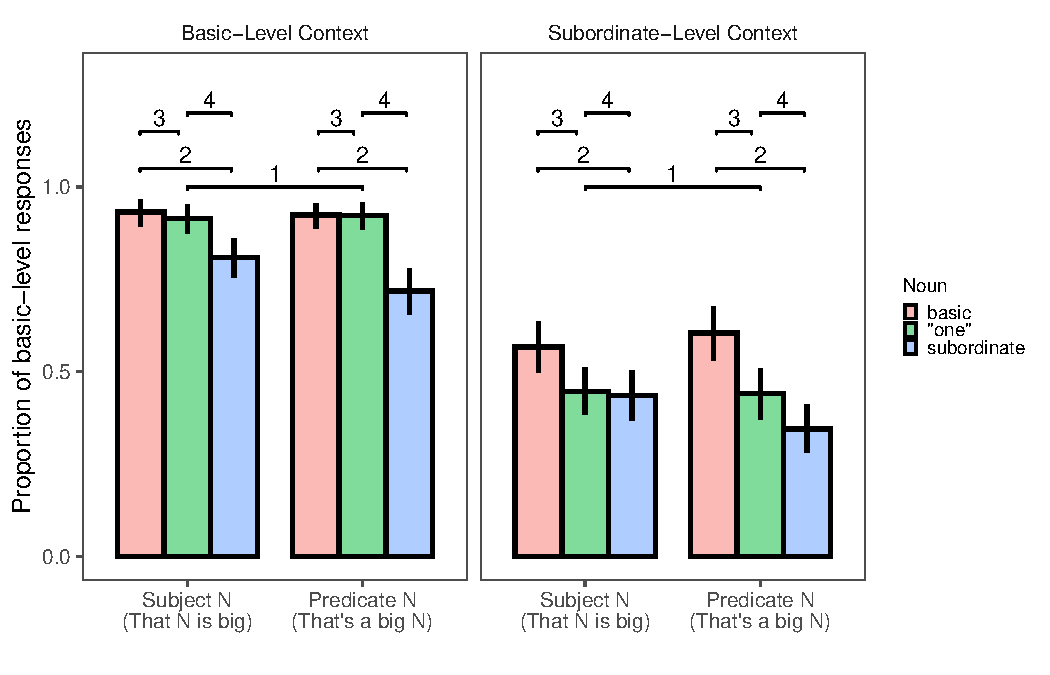
\includegraphics[width=0.7\linewidth]{expt3-cc-inference-wSigLines.pdf}
	\end{center}
	\vspace{-0.3cm}
	\caption{Experiment 3 results: Proportions of inferred comparison classes in terms of basic-level responses (e.g.,~“...big relative to other dogs”), depending on syntactic position of the noun (x-axis), noun-label (color), and context (facets).
		Context strongly modulated the comparison class (left~vs.~right panel). 
		The noun additionally provided a cue to the comparison class (red~vs.~blue) bars, regardless of syntactic position. 
		The effect of noun (red~vs.~blue) is modulated by syntax. 
		Error-bars denote bootstrapped 95\% confidence intervals.}
	\label{cci-results}
\end{figure*}
Participants’ responses were manually classified into basic-level and subordinate comparison classes. 4 superordinate comparison classes were collapsed with the basic-level responses. 39 (1.6\%) uncategorizable responses were excluded from the analysis. 
A Bayesian logistic mixed-effects regression model was used, regressing the response category against the syntactic condition (subject-N~vs.~predicate-N), the noun category (basic~vs.~subordinate~vs.~‘one’), the context (basic~vs.~subordinate), their two-way and three-way interactions and maximal random effect structure appropriate for this experimental design.\footnote{In brm-style syntax: \texttt{response\_category $\sim$ syntax*NP*context + (1 + syntax + NP + context || subject) + (1 + syntax*NP*context || target)}. Correlations of random effects were set to 0 for computational tractability.} Default priors were used.
The predictors were sum-coded: predicate-N and basic-level context were coded as 1, subject-N and subordinate context as -1; the basic-level and the subordinate noun-levels were coded against the baseline anaphoric `one'. 

The results indicate that participants flexibly adjust the inferred comparison class according to many factors. First, a large effect of visual context going above and beyond other factors was found ($\beta = \rlgetnum{expt3_full_brm_revised2.csv}{Rowname}{context_sum}{Estimate}{2} [\rlgetnum{expt3_full_brm_revised2.csv}{Rowname}{context_sum}{l.95..CI}{2},  \rlgetnum{expt3_full_brm_revised2.csv}{Rowname}{context_sum}{u.95..CI}{2}]$; Fig.~\ref{cci-results}, left~vs.~right facets), supported by the inferences drawn from the baseline condition anaphoric ‘one’ ($\beta = \rlgetnum{expt3_3way_full_contrasts_wProbs.csv}{Rowname}{context_one_v_mean}{mean}{2} [\rlgetnum{expt3_3way_full_contrasts_wProbs.csv}{Rowname}{context_one_v_mean}{X.95.}{2}, \rlgetnum{expt3_3way_full_contrasts_wProbs.csv}{Rowname}{context_one_v_mean}{u95.}{2}]$; Fig.~\ref{cci-results}, comparison 1, left~vs.~right facet): %green bars in the left~vs.~right facet): 
participants were appreciably more likely to infer basic-level comparison classes given a basic-level context, compared to a subordinate context. Furthermore, an effect of the noun on inferred comparison classes regardless of its position in the sentence was found: participants were more likely to infer basic-level comparison classes from basic-level nouns than from subordinate nouns ($\beta = \rlgetnum{expt3_3way_full_contrasts_wProbs.csv}{Rowname}{basic_v_sub}{mean}{2} [\rlgetnum{expt3_3way_full_contrasts_wProbs.csv}{Rowname}{basic_v_sub}{X.95.}{2}, \rlgetnum{expt3_3way_full_contrasts_wProbs.csv}{Rowname}{basic_v_sub}{u95.}{2}$]; Fig.~\ref{cci-results}, comparison 2). The noun-effects can be observed on top of effects of the visual context indicated by the baseline condition `one': participants inferred more basic-level comparison classes from basic-level nouns than from `one', and less from subordinate nouns than from `one' (basic-level~vs.~`one': $\beta = \rlgetnum{expt3_3way_full_contrasts_wProbs.csv}{Rowname}{basic_v_one}{mean}{2} [\rlgetnum{expt3_3way_full_contrasts_wProbs.csv}{Rowname}{basic_v_one}{X.95.}{2}, \rlgetnum{expt3_3way_full_contrasts_wProbs.csv}{Rowname}{basic_v_one}{u95.}{2}]$, Fig.~\ref{cci-results} comparison 3; and subordinate~vs.~`one': $\beta = \rlgetnum{expt3_3way_full_contrasts_wProbs.csv}{Rowname}{sub_v_one}{mean}{2} [\rlgetnum{expt3_3way_full_contrasts_wProbs.csv}{Rowname}{sub_v_one}{X.95.}{2}, \rlgetnum{expt3_3way_full_contrasts_wProbs.csv}{Rowname}{sub_v_one}{u95.}{2}]$, Fig.~\ref{cci-results} comparison 4). 
Notably, the subordinate comparison class was the minority response even given a subordinate noun in the basic-level context, speaking against a compositional view of adjective comparison classes, wherein the noun would always set the comparison class (Fig. \ref{cci-results}; blue bars, left facet). Even in the subordinate context inferences drawn from the subordinate noun were not exclusively subordinate comparison classes, indicating a basic-level bias \parencite[Fig.~\ref{cci-results}; blue bars, right facet; cf.][]{rosch1976, graf2016animal}. 

Crucially, a credible syntax-by-noun interaction was found, supporting predictions provided by the reference-predication trade-off hypothesis: more subordinate comparison classes were inferred from subordinate nouns appearing in predicate position than in the subject position, compared to basic-level nouns (Fig.~\ref{cci-results} comparison 2 $\times$ x-axis; $\beta = \rlgetnum{expt3_3way_full_contrasts_wProbs.csv}{Rowname}{syntax_basic_v_sub}{mean}{2} [\rlgetnum{expt3_3way_full_contrasts_wProbs.csv}{Rowname}{syntax_basic_v_sub}{X.95.}{2}, \rlgetnum{expt3_3way_full_contrasts_wProbs.csv}{Rowname}{syntax_basic_v_sub}{u95.}{2}]$). Examining the interaction by-noun, preliminary evidence was found that the interaction is primarily driven by the subordinate noun: a $\rlgetnum{expt3_3way_full_contrasts_wProbs.csv}{Rowname}{syntax_sub_v_one}{prob_lt_0}{1}$\% probability was found that the subordinate-N~vs.~`one' $\times$ syntax interaction term was less than 0 (i.e., more subordinate comparison classes were inferred when the noun was in the predicate; $\beta = \rlgetnum{expt3_3way_full_contrasts_wProbs.csv}{Rowname}{syntax_sub_v_one}{mean}{2} [\rlgetnum{expt3_3way_full_contrasts_wProbs.csv}{Rowname}{syntax_sub_v_one}{X.95.}{2}, \rlgetnum{expt3_3way_full_contrasts_wProbs.csv}{Rowname}{syntax_sub_v_one}{u95.}{2}]$), in contrast to only a $\rlgetnum{expt3_3way_full_contrasts_wProbs.csv}{Rowname}{syntax_basic_v_one}{prob_gt_0}{1}$\% probability of the basic-N~vs.~`one' $\times$ syntax interaction being greater than 0 (i.e., more basic-level comparison classes inferred when the noun was in the predicate; $\beta = \rlgetnum{expt3_3way_full_contrasts_wProbs.csv}{Rowname}{syntax_basic_v_one}{mean}{2} [\rlgetnum{expt3_3way_full_contrasts_wProbs.csv}{Rowname}{syntax_basic_v_one}{X.95.}{2}, \rlgetnum{expt3_3way_full_contrasts_wProbs.csv}{Rowname}{syntax_basic_v_one}{u95.}{2}]$). This effect was even more pronounced under an exploratory model, assuming only a two-way syntax-by-noun interaction and a main effect of context: the probability was $\rlgetnum{expt3_2way_full_contrasts_wProbs.csv}{Rowname}{syntax_sub_v_one}{prob_lt_0}{1}$\% for the subordinate noun~vs.~`one' $\times$ syntax estimate to be less than 0.\footnote{Exploratory model: \texttt{response\_category $\sim$ syntax*NP + context + (1 + syntax + NP + context || subject) + (1 + syntax*NP + context || target)}} This is consistent with the reference-predication trade-off hypothesis, predicting that an effect of syntax is more pronounced for nouns with higher referential utility, which is generally the case for subordinate compared to basic-level nouns, especially in the basic-level context \parencite[cf.][]{graf2016animal}.

Taking the reference-predication trade-off hypothesis even further, another exploratory analysis suggested that participants might consider informational functions of the noun irrespective of the syntactic position. In particular, when a noun in the subject is referentially uninformative they might reason that this noun too is intended for predication. For instance, the subordinate context yields the basic-level target label referentially uninformative (all members of context can be described by the basic-level noun), such that listeners might reason about the presence of the noun as intended to convey the comparison class when it appears in both subject or predicate position. In line with this idea, in the subordinate context condition a higher rate of basic-level comparison classes was inferred from the basic-level noun compared to `one' ($\rlgetnum{expt3_subContext.csv}{Rowname}{basic_v_one}{prob_gt_0}{1}$\% of the credible interval of the basic~vs.~`one' estimate was greater than 0: $\beta = \rlgetnum{expt3_subContext.csv}{Rowname}{basic_v_one}{mean}{2} [\rlgetnum{expt3_subContext.csv}{Rowname}{basic_v_one}{X.95.}{2}, \rlgetnum{expt3_subContext.csv}{Rowname}{basic_v_one}{u95.}{2}]$; Fig. \ref{cci-results}; comparison~3, right facet), indicating an effect of the basic-level noun going beyond contextual resolution of this referentially underspecified expression, as in case of `one'.%and more subordinate comparison classes were inferred from subordinate labels comapred to 'one' ($\rlgetnum{expt3_subContext.csv}{Rowname}{sub_v_one}{prob_lt_0}{1}$\% of the credible interval of the subordinate~vs.~'one' estimate was smaller than 0: $\beta = \rlgetnum{expt3_subContext.csv}{Rowname}{sub_v_one}{mean}{2} [\rlgetnum{expt3_subContext.csv}{Rowname}{sub_v_one}{X.95.}{2}, \rlgetnum{expt3_subContext.csv}{Rowname}{sub_v_one}{u95.}{2}]$;Fig. \ref{cci-results}; blue~vs.~green bars, right facet), across syntactic frames.
\footnote{These contrasts were computed on data subsetted by context}
The data observed in the basic-level context is also consistent with the hypothesis that the referentially uninformative noun in the subject signals the comparison class, but the referentially-uninformative basic-level label condition and the baseline `one' are both subject to a ceiling effect and hence leave no room for any effects beyond baseline.  

These empirical results provide a comprehensive picture of syntactic and pragmatic effects contributing to comparison class inference. In particular, this experiment shows that the same utterances are interpreted differently in distinct contexts, as evidenced by the large effect of context. This speaks against purely syntactic or semantic views arguing that meaning of utterances is fully specified by their words (as discussed in Section \ref{2.3.}). Furthermore, the influence of the noun in the utterance independent of context and syntactic position confirms that the noun is a salient cue to the comparison class, yet insufficient on its own to account for interpretative differences observed. Finally, evidence consistent with the reference-predication hypothesis is found, suggesting that humans integrate the referential utility with contextual cues when reasoning about the contribution of the noun to the comparison class (as shown by the noun $\times$ syntax interaction). The data suggests that one-dimensional theories of gradable adjective interpretation do not account for flexible comparison class inference; humans integrate both pragmatic and syntactic information to felicitously use gradable adjectives across different contexts. 

\section{Experiment 4: Direct Modification Experiment} 
However, in order to keep a simple operationalization of the reference-predication distinction, a potential confound was introduced in experiments 1-3. The position of the noun was perfectly confounded with whether the noun was directly syntactically modified by the adjective (predicate-N condition) or not (subject-N condition). Therefore, experiments 1-3 did not allow to rule out that the observed interpretative differences were not due to the differing modification, as discussed in Section \ref{2.3.}.  Yet the reference-predication trade-off view predicts that referential pressure takes off predicational weight from the noun used for reference and therefore decreases its strength in constraining the comparison class, independent of the syntactic modification --- informational goals are suggested to be the primary driving force above syntactic phenomena. This prediction was investigated in this direct-modification experiment \parencite{TesslerEtAl2020AMLaP}.

The main idea of this study was to manipulate the position of the noun while the modification was constant across the positions. Therefore, in critical trials the position of the critical noun in the sentence was varied and the noun was always directly modified by the adjective \textit{big} or \textit{small} (i.e., 'big Great Dane', 'small pug'). The critical nouns were always subordinate referent labels. In order to create maximally symmetric syntactic manipulations of the critical sentences, a second noun was used which described a visually salient feature of the referent. For example, the referents for one of the dog contexts were prize-winners, as indicated by prize-bows depicted on the referents (Table~\ref{stims:e4}). So the critical sentence was either “That prize-winner is a big Great Dane” (predicate-N) or “That big Great Dane is a prize-winner” (subject-N). For the same reason of manipulation symmetry nouns were chosen to describe this feature, as opposed to e.g.~adjectives (``That big Great Dane is my favourite"~vs.~``??That my favourite is a big Great Dane"). The features were chosen such that they were visually accessible, describable by a noun and would be part of the referent.   
The referents appeared in a basic-level context, which included two other members of the same subordinate category as the referent, and two other individuals with the feature described by the second noun of the sentence: e.g., in the dog-context there were two other prize-winners (Fig.~\ref{double-mod-main}). Because the reference-predication trade-off is based on explaining away a noun via its potential referential use, through this contextual manipulation the referential utilities of the two nouns of the sentence were equal, such that only the noun’s syntactic position and combination with the deictic ‘that’ could provide a cue towards referential intention. Therefore, the critical subordinate noun is expected to constrain the inferred comparison class more strongly when it appears in the predicate of the sentence rather than in the subject. 

\begin{table}[t]
	\small{
		\begin{center}
			\caption{E4 experimental items: each basic-level context had two potential targets from an either saliently small or saliently big subordinate category within the basic-level class. Each category had a corresponding context cover story which was comleted by ``...and you see the following:". The referents had an additional visually salient feature, described by the second noun in critical sentences (N2).}
			\label{stims:e4}
			\vskip 0.12in
			\fontsize{10}{11}\selectfont
			\setlength{\extrarowheight}{.5em}
			\begin{tabularx}{\textwidth}{>{\hsize=.6\hsize}X>{\hsize=.8\hsize}X>{\hsize=.8\hsize}X>{\hsize=2\hsize}X>{\hsize=.8\hsize}X}
				\hline
				Basic-level \newline category & Smaller \newline referent & Bigger \newline referent & Context & Visual \newline feature / N2\\
				\hline
				Dogs & Pug & Great Dane & You and your friend are at a pet show. & Prize-winner \\
				Dogs & Chihuahua & Doberman & You and your friend are at an animal training ground. & Service-animal\\
				Birds & Hummingbird & Eagle & You visit your friend who works at an animal shelter. & Rescue  \\
				Flowers & Dandelion & Sunflower & You and your friend are at their garden. & Gift\\
				Trees & Bonsai & Redwood & You and your friend walk to their cabin in a park for the first time. You want to memorize the path. & Landmark\\
				\hline     
			\end{tabularx}
		\end{center}
	}
\end{table}

\begin{figure*}[t]
	\begin{center}
		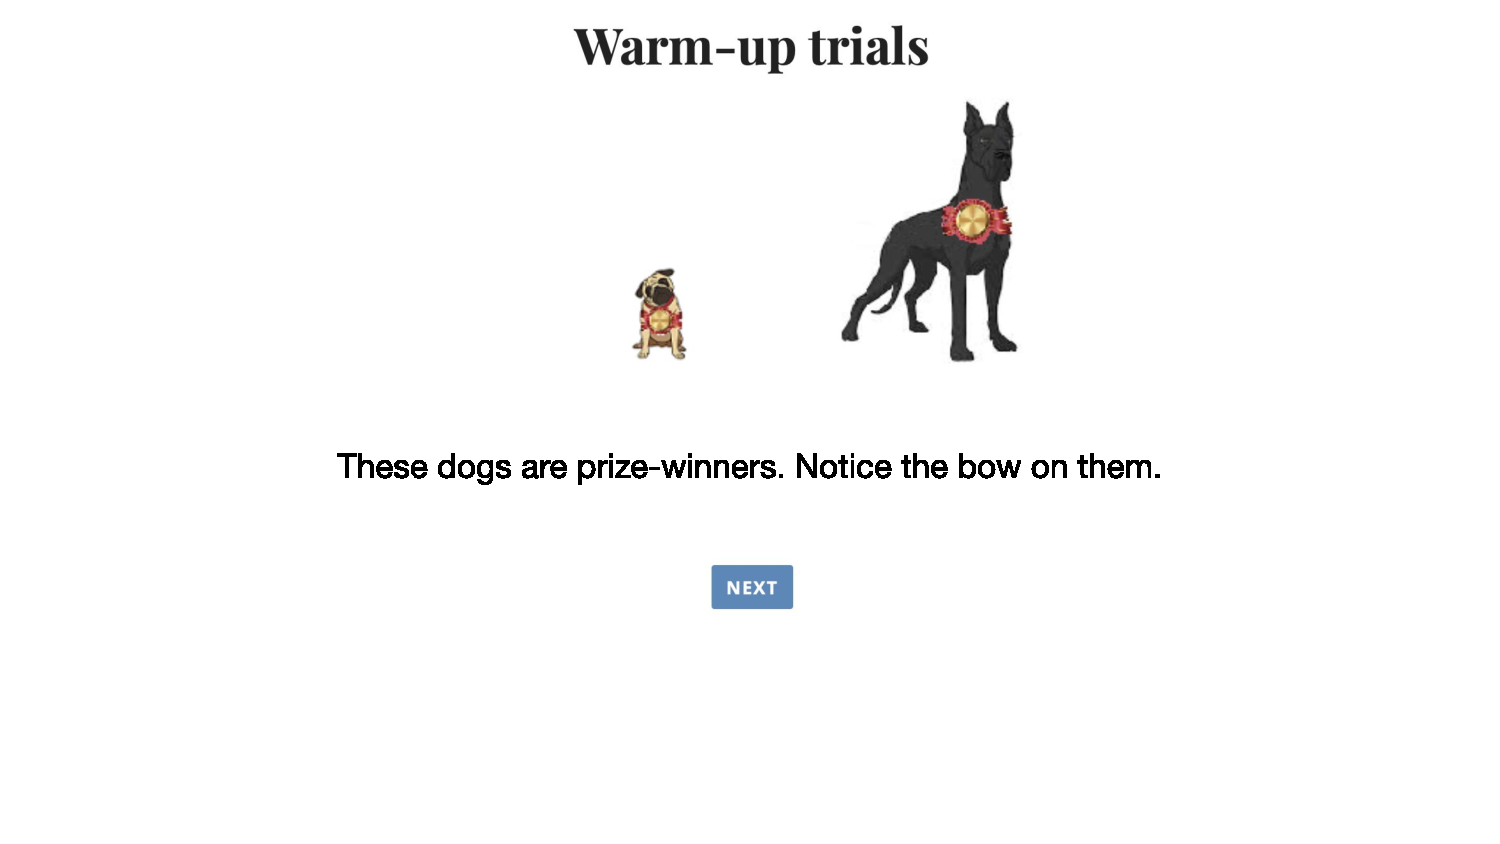
\includegraphics[width=\linewidth]{screenshots/direct-mod-N2-warmup.pdf}
	\end{center}
	\vspace{-2cm}
	\caption{Experiment 4 feature demonstration trial: Participants learn about additional features of the referents used on one critical main trial. For the dog-context participants learn that the pug and the Great Dane are prize-winners, indicated by bows on them.}
	\label{double-mod-N2warmup}
\end{figure*} 
The experimental set-up was similar to Experiment 3. Five different contexts were used in this experiment: there were two dog contexts, a flower, a bird and a tree context (Table \ref{stims:e4}). Four out of five contexts were randomly sampled for each participant.  Participants completed two experimental blocks, each consisting of warm-up and main trials using two of the sampled categories. In the first block, participants first completed two rounds of labeling warm-up trials. A round consisted of a demonstration trial where participants saw two subordinate members of a basic-level category used in this block and read their labels. For example, they saw pictures of a Great Dane and a pug next to each other and read “This is a Great Dane” and “This is a pug”, respectively. They could proceed after 3.5 seconds to the next trial where they had to label other instances of the same categories themselves. They also had to provide a common label for the pictures (i.e., dogs; see Fig.~\ref{warmup-production}). The order of the pictures was randomized between-participants. They were provided feedback on their labels and could proceed only after correcting their labels.  After two labeling warm-up rounds, participants completed two demonstration trials of at least 3.5 seconds each, learning about the additional features of the referents described by the second noun of the critical sentences in main trials (Table \ref{stims:e4}). For example, participants saw a picture depicting the Great Dane and the pug with prize-bows, and read: “These dogs are prize-winners. Notice the bow on them.” (Fig.~\ref{double-mod-N2warmup}). Finally, participants completed a comparison class paraphrase practice trial, identical to the one used in Experiment 3. The warm-up trials in the second experimental block were identical, but there was no paraphrase practice trial.  

\begin{figure*}[t]
	\begin{center}
		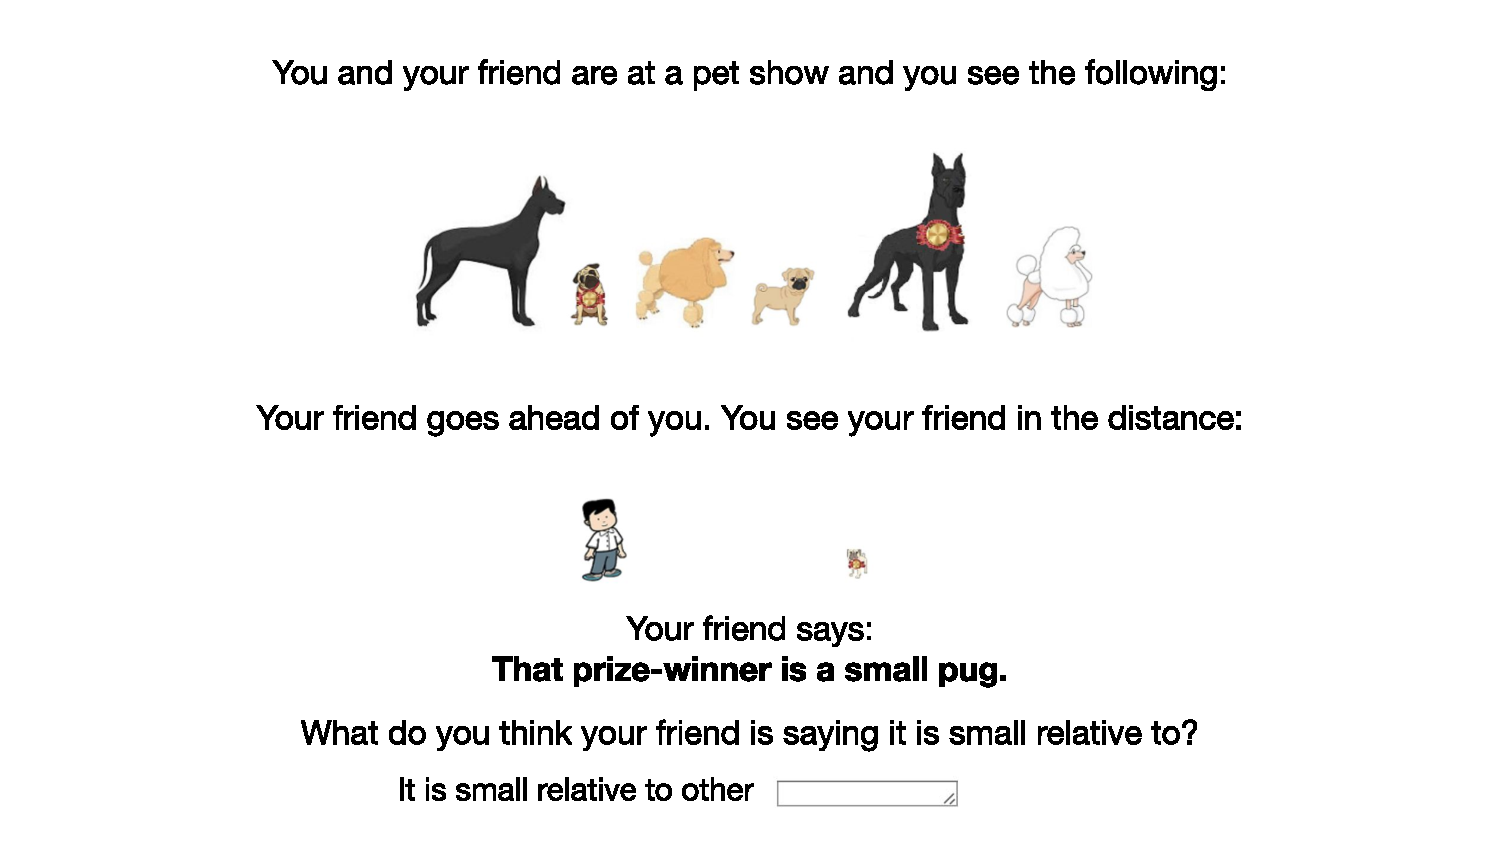
\includegraphics[width=\linewidth]{screenshots/double-mod-main.pdf}
	\end{center}
	\vspace{-0.5cm}
	\caption{Example critical main trial in Experiment 4: Participants see a dog-context and read the corresponding cover story. The small-subordinate referent is described by a predicate-noun sentence.}
	\label{double-mod-main}
\end{figure*} 
Then, participants completed four main trials --- two critical and two filler trials, in randomized order, where a filler trials was always the first trial of the block. In the critical trials, a subordinate referent with an additional feature (e.g., a prize-winner bow) appeared in the corresponding context, as described above (Fig.~\ref{double-mod-main}). Participants read different cover stories for each context (Table \ref{stims:e4}).  For example, for a dog context, they read “You and your friend are at a pet show and you see the following:” above the context picture. Below, they read “Your friend runs far ahead of you. You see your friend in the distance:”, followed by a depiction of the referent with the additional feature next to a person; to induce the illusion of distance, both were small relative to the context picture. Then they read “Your friend says:”, followed by the critical sentence. Finally, they were asked: “What do you think your friend is saying it is \{big / small\} relative to?”, introducing the paraphrase template, like in Experiment 3. For a given category, one of the possible targets appeared in this critical trial (e.g., the Great Dane). The other possible target (i.e., the pug) then appeared in a filler trial in the same block. Filler trials were identical to main trials with basic-level contexts and subordinate nouns from Experiment 3. The referent-size (i.e., large-subordinate vs. small-subordinate) was counterbalanced across syntactic conditions and trial types within-participant, resulting in eight unique conditions. Each participant saw each condition once, resulting in eight main trials.\footnote{The experimental design described here is the final design which will be used in the main study. This design was used in the last pilot where 36 participants were recruited. The preceding pilot where 17 participants were recruited only differed from the described design in that there were no feature demonstration trials, participants did not provide common labels in the labeling warm-ups and the conditions were not counter-balanced across referent-sizes.}

%\pt{Include predictions and numerical expectations; include note about differences bw pilot 5 and 6: warm-up trials in pilot 5 had no basic-level labelling task.}

According to the reference-predication hypothesis, participants should be more likely to take the noun as signalling the comparison class when it appears in the predicate than when it appears in the subject \emph{irrespective} of modification. That is, in the critical trials where the noun is always directly modified by the adjective, a higher proportion of subordinate comparison classes is expected to be inferred in the predicate condition, compared to the subject condition. A positive credible regression coefficient for the respective contrast would support this prediction. Further, since the filler condition replicates the condition of interest from Experiment 3, the same pattern is expected for those trials. Therefore, no difference is expected between the trial types, such that the respective regression coefficient for the trial effect is not expected to be credible.     

\subsection{Participants}
The results reported here were gathered from \rlgetvariable{myvars-direct-mod.csv}{nSubj} participants recruited in two pilot studies.\footnote{The number of participants for the main experiment was determined via a Bayesian power analysis and revealed that 300 participants are required for a power $>$ 0.85 \parencite{kruschke2014doing, powerKurz}. The main study is in progress.} \rlgetvariable{myvars-direct-mod.csv}{nExcludedTotal} participants were excluded for indicating a native language other than English, or failing either the comparison class inference practice trial or the labeling warm-up trials more than four times upon correction. The experiment took about 7 minutes and participants were compensated \$1.00. If partial data was missing from a participant, available data was used for analyses.   
 
\subsection{Results}
\begin{figure*}[t]
	\begin{center}
		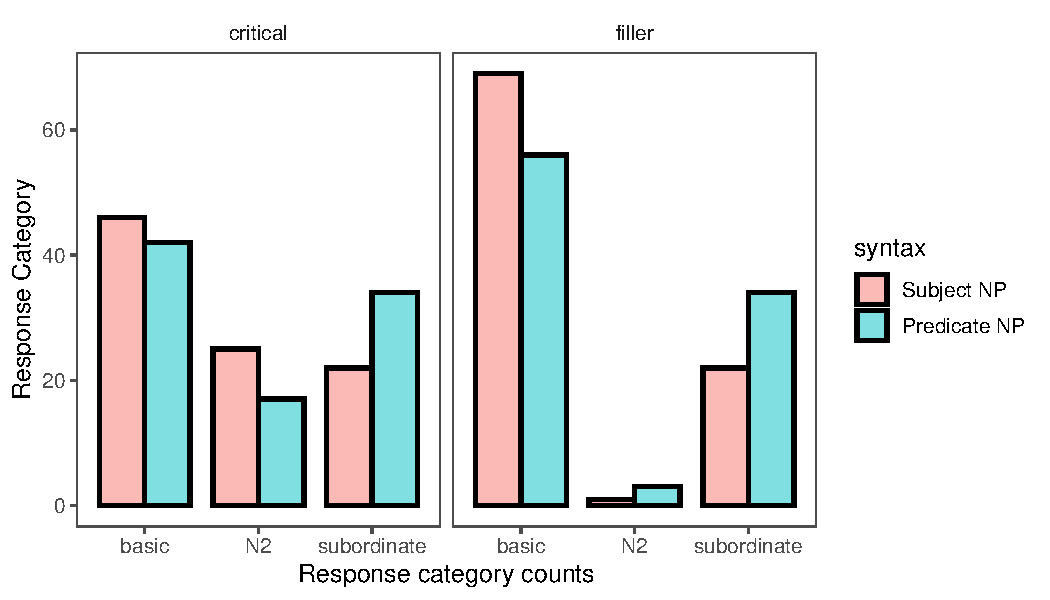
\includegraphics[width=0.8\linewidth]{double_mod_resp_counts.pdf}
	\end{center}
	\vspace{-0.3cm}
	\caption{Response categories produced in the Experiment 4 pilot: Counts of different response types (basic-level target labels, subordinate target labels, N2 denoting the visual feature in critical trials; x-axis) when the subordinate noun occured in different positions (color),  by trial type (facets).}
	\label{double-mod-resp-counts}
\end{figure*}

\begin{figure*}[h]
	\begin{center}
		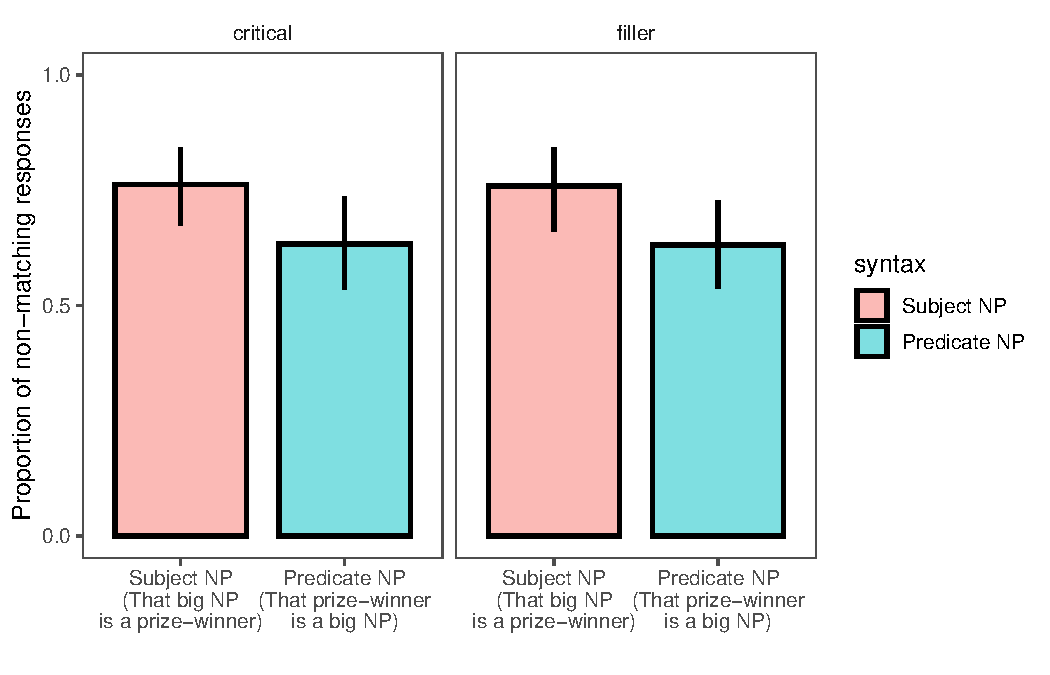
\includegraphics[width=0.7\linewidth]{double_mod.pdf}
	\end{center}
	\vspace{-0.3cm}
	\caption{Experiment 4 pilot results: Proportions of inferred comparison classes in terms of responses not matching the critical subordinate target label (e.g.,~“...big relative to other dogs/prize-winners/animals”), depending on syntactic position of the noun (x-axis) and trial-type (facets). Error-bars denote bootstrapped 95\% confidence intervals.}
	\label{double-mod-results}
\end{figure*}


Participants' responses were manually classified into responses matching the critical subordinate referent label noun (i.e. subordinate comparison classes) and non-matching responses. That is, non-matching responses included basic-level or superordinate nouns as well as the second supplementary feature-nouns (e.g., ``...relative to other prize-winners"). Compound modified nouns were classified according to the head noun: for instance, responses like ``prize-winning Great Danes" were classified as matching, and responses like ``floral gifts" were classified as non-matching. The overall proportion of responses matching the supplementary feature-nouns was 12.4 \%, and more of these nouns were provided when this noun appeared in the predicate than in the subject position (Fig.~\ref{double-mod-resp-counts}). 
13 uncategorizable responses (3.4\%) were excluded from analysis. 
A Bayesian logistic mixed-effects regression model was used, predicting the response category from the syntactic condition (subject-N~vs.~predicate-N), the trial type (critical~vs.~filler) and their two-way interaction. By-participant and by-item random intercepts and random slope effects of both predictors and their interaction were included.\footnote{In brm-style syntax: \texttt{response\_category $\sim$ syntax*trial\_type + (1 + syntax*trial\_type | subject) + (1 + syntax*trial\_type | target)}}  
Default priors were used. The predictors were sum-coded, coding the subject-N syntax and filler trials as 1, the predicate-N syntax and critical trials as -1.%\footnote{Preliminary results of this experiment from a different pilot were presented as a poster at AMLaP 2020 \parencite{TesslerEtAl2020AMLaP}. }

In line with predictions made by the reference-predication trade-off hypothesis, participants were sensitive to the syntactic position of the noun irrespectively of syntactic modification: even given directly modified nouns, in the critical trials pariticipants were more likely to infer the subordinate comparison class when the subordinate noun phrase appeared in the predicate compared to the subject position ($\beta = \rlgetnum{expt4_contrasts.csv}{Rowname}{syntax_critical}{mean}{2} [\rlgetnum{expt4_contrasts.csv}{Rowname}{syntax_critical}{lower}{2},  \rlgetnum{expt4_contrasts.csv}{Rowname}{syntax_critical}{upper}{2}]$; Fig.~\ref{double-mod-results}, left facet). 
Furthermore, supporting the findings from Experiment 3, in the filler trials participants also tended to infer more subordinate comparison classes from subordinate nouns in the predicate rather than in the subject position (the probability was $\rlgetnum{expt4_contrasts.csv}{Rowname}{syntax_filler}{prob_gt_0}{2}$\% that the estimate was greater than 0: $\beta = \rlgetnum{expt4_contrasts.csv}{Rowname}{syntax_filler}{mean}{2} [\rlgetnum{expt4_contrasts.csv}{Rowname}{syntax_filler}{lower}{2},  \rlgetnum{expt4_contrasts.csv}{Rowname}{syntax_filler}{upper}{2}]$; Fig.~\ref{double-mod-results}, right facet). Overall, participants inferred more subordinate comparison classes when the subordinate noun appeared in the predicate than when it appeared in the subject, across trial types ($\beta = \rlgetnum{expt4_contrasts.csv}{Rowname}{syntax_subj_v_pred}{mean}{2} [\rlgetnum{expt4_contrasts.csv}{Rowname}{syntax_subj_v_pred}{lower}{2},  \rlgetnum{expt4_contrasts.csv}{Rowname}{syntax_subj_v_pred}{upper}{2}]$). Consistent with the prediction that syntactic modification which was varied between trial types should not play a role for comparison class inference, no credible effects of trial type or difference in syntax-effects on different trial-types were observed (trial effect: $\beta = \rlgetnum{expt4_contrasts.csv}{Rowname}{trial_filler_v_critical}{mean}{2} [\rlgetnum{expt4_contrasts.csv}{Rowname}{trial_filler_v_critical}{lower}{2},  \rlgetnum{expt4_contrasts.csv}{Rowname}{trial_filler_v_critical}{upper}{2}]$, Fig.~\ref{double-mod-results}, left~vs.~right facet; trial $\times$ syntax interaction estimate: $\beta = \rlgetnum{expt4_contrasts.csv}{Rowname}{b_syntax_sum1:trial_sum1}{mean}{2} [\rlgetnum{expt4_contrasts.csv}{Rowname}{b_syntax_sum1:trial_sum1}{lower}{2},  \rlgetnum{expt4_contrasts.csv}{Rowname}{b_syntax_sum1:trial_sum1}{upper}{2}]$, Fig.~\ref{double-mod-results}, left~vs.~right bar in left~vs.~right facet).  

This experiment provided evidence that participants are able to flexibly reason about informational goals the nouns combining with the adjective are intended for, above and beyond syntactic modification. These results show that the primary driver behind the cue-strength of the noun towards the comparison class is indeed the informational goal that the noun accomplishes, and not the modification of the noun by the adjective.  Therefore, it can be ruled out that nouns appearing in the predicate position of the utterance provided a stronger cue towards the comparison class than nouns in the subject just due to direct modification by the adjective (cf. experiments 1-3). 

Together with Experiment 3, these results show that listeners flexibly adjust their comparison classes by reasoning about informational goals and sentence structure, integrated with perceptual cues and their general world knowledge.   
   


\chapter{A Bayesian Reference-Predication Model}
\label{chapter05}
Vagueness and context-dependence of gradable adjectives have been promisingly formalized in computational models within the Rational Speech Act framework -  a suite of game-theoretically oriented recursive models of pragmatic language understanding \parencite[e.g.,][]{goodman2016, lassiter2017adjectival, tessler2017warm}. Introduced by \textcite{frank2012predicting}, the Rational Speech Act framework is well in line with recent insights in Bayesian cognitive modelling, showing a great deal of flexibility to account for various phenomena studied in pragmatics like scalar implicature, hyperbolic language or generics, among many others \parencite[e.g.,][]{tenenbaum2011grow, problang}. This chapter reviews the basics of Rational Speech Act models and specifically prior models of gradable adjectives. While accounting for many aspects of gradable adectives, many of those models assumed an a priori fixed comparison class. Yet as shown empirically in the previous Chapter \ref{chapter04}, listeners flexibly reason about the intended comparison class by taking into account syntactic and contextual cues. Therefore, this chapter attempts to propose a minimal extension to existing RSA-models which will formalize the reference-predication trade-off hypothesis of comparison class inference.%, allowing to flexibly incorporate reasoning about context and role of the noun in comparison class inference. 
  
\section{Understanding Rational Speech Act Models}
\label{intro-rsa}
Language is fascinatingly flexible and efficient, and largely so because interlocutors do not have to explicitly encode all information in utterances they produce, but instead rely on each other's ability to infer many aspects of the message from linguistic and situational context. In particular, pragmatic models of communication posit that given these contextual constrains, speakers and listeners can efficiently \emph{reason about each other's intended meaning of utterances} under one important assumption: speakers are approximately \emph{rational} with respect to their communicative goals \parencite{frank2012predicting}. The Rational Speech Act framework (henceforth: RSA) views this process of establishing the intended meaning as recursive reasoning between speaker and listener: in interpretation-oriented models, a pragmatic listener $L_1$ infers a state of the world intended to be conveyed by a rational speaker $S_1$, by using \emph{Bayesian inference} to reason about likely world states given the observed utterance, given that the speaker $S_1$ chooses utterances according to their most likely semantic interpretation by a literal listener $L_0$ \parencite{problang}.  

The idea of language as rational action produced by \emph{cooperative} interlocutors was formulated by \textcite{grice1975logic}. The core of his proposal are four conversational maxims that speakers are thought to stick to when producing utterances in order to convey particular messages: the \emph{maxims of relation} (contributions made to the conversation are relevant), \emph{quantity} (the contributions are as informative as required, but not more so), \emph{quality} (the speaker believes their contributions to be true) and \emph{manner} (the way the contributions are expressed is perspicuous). Listeners then reason about intended messages in light of these maxims \parencite{grice1975logic}.

Grice’s ideas became particularly influential when precise information-theoretic formalisations of such vague concepts like \emph{informativeness, cooperation} and \emph{relevance} were proposed, and, informed by insights from game-theory, gave rise to RSA \parencite{frank2012predicting}.
In particular, RSA captures cooperative coordination of intended meaning between interlocutors via recursive application of probabilistic mechanisms; and relevance or informativeness of utterances is captured as the \emph{utility} of the utterance in helping the listener reduce uncertainty in their beliefs about the world, where these beliefs can be represented as a probability distribution over possible states of the world \parencite[as advocated by e.g.][]{tenenbaum2011grow}.  
That is, listeners update their beliefs about the world via Bayes' rule upon hearing an utterance produced by an informative speaker \parencite{frank2012predicting}.\footnote{Familiarity with basic notions in probability and Bayesian inference is presupposed here. For a review of aspects relevant for RSA, \textcite[see e.g.][]{lassiter2017adjectival}.}

The mechanisms of RSA are best illustrated by a simple example from a reference game, described by \textcite{frank2012predicting}.
Consider a simple world consisting of a context $C$ = \{blue square, blue circle, green square\} (Fig. \ref{rsa-scene}).
\begin{figure*}[t]
	\begin{center}
		
\includegraphics[width=0.5\linewidth]{rsa_scene.png}
	\end{center}
	\vspace{-0.3cm}
	\caption{A simple reference resolution example scenario: the context $C$ consists of three possible referents \parencite{frank2012predicting}}
	\label{rsa-scene}
\end{figure*}
In a reference game scenario, a speaker wants to communicate to a listener a particular referent $s$ in context $C$, e.g., the blue square. To do so, she has a finite set of utterances $U = \{blue, green, square, circle\}$.\footnote{The finite fixed set of alternative utterances is a crucial assumption made in RSA. It is an important question for future research how interlocutors actually determine this set of relevant alternatives.} A listener then tries to recover the intended referent (i.e., the blue square) upon receiving an utterance (e.g., "blue"). 
As mentioned above, standard RSA models consist of three layers: a pragmatic speaker $S_1$ who chooses an optimal utterance for signalling $s$ (the blue square) to a literal listener $L_0$, who infers all the referents consistent with the literal meaning of the utterance $u$ ('blue'), and a pragmatic listener $L_1$ who reasons about this speaker behaviour given a particular utterance $u$ ('blue'), using Bayes' rule.

So the basis of RSA models is the na\"ive literal listener agent $L_0$ that $S_1$ reasons about when choosing an optimal utterance to communicate the blue square, who computes a probability distribution over possible referents in context $C$  consistent with the received utterance $u$: %\pt{function that maps each utterance to the probability distribution over world states}
\begin{equation}
P_{L_0}(s \mid u, C) = \frac{\llbracket u \rrbracket (s) \times P(s)}{\sum_{s' \in C} \llbracket u \rrbracket (s') P(s')}
\end{equation}
The context $C$ is typically assumed to be shared between speaker and listener, so it will be dropped in further derivations for simplicity. Given that the denominator is a constant, it can also be dropped for simplicity, so that the probability of a particular state $s$ given utterance $u$ is \emph{proportional} to the literal meaning $\llbracket u \rrbracket (s)$ and the prior probability of $s$: 
\begin{equation}
P_{L_0}(s \mid u) \propto \llbracket u \rrbracket (s) \times P(s)
\end{equation}
The prior $P(s)$ is the prior belief of $L_0$ about which states are likely to be communicated by the speaker. Typically, a uniform prior is used, indicating that a priori any state is as likely as others, but relevant contextual information like perceptual salience or frequency of some referents might be encoded in this prior \parencite{frank2012predicting}.

The second component of the $L_0$ is the \emph{literal meaning} of the observed utterance $u$ (indicated as $\llbracket u \rrbracket$). In RSA, literal semantics computation is based on a form of Montague’s compositional semantics, typically assuming a mapping from particular states to Boolean truth-values \parencite{montague1973proper} \parencite[but see e.g.][for alternative approaches]{degen2020redundancy}. 
So, for instance for the context Fig. \ref{rsa-scene}, applying the utterance 'circle' to the blue square would return \texttt{false}, but 'blue' would be \texttt{true}:
\begin{align}
\llbracket circle \rrbracket (blue \: square) = 0 \notag \\
\llbracket blue \rrbracket (blue\: square) = 1
\end{align}
  
So for our example utterance 'blue' the literal listener $L_0$ infers a uniform distribution over the blue circle and the blue square, since the utterance equally applies to both objects (Table \ref{rsa-l0}):

\begin{table}[h]
	\begin{center}
		\caption{The probability distribution over states inferred by $L_0$ when hearing the utterance 'blue' in context $C$.}
		\label{rsa-l0}
		\vskip 0.12in
		\begin{tabular}{cc}
			State & Probability \\
			\hline
			blue circle & 0.5 \\
			blue square & 0.5 \\
			\hline
		\end{tabular}
	\end{center}
\end{table}

The next RSA layer is the pragmatic speaker $S_1$. $S_1$ is modelled as an agent who chooses an utterance $u$ rationally, i.e., according to its expected utility, in order to communicate a particular state of the world $s$ in context $C$ to $L_0$. This is captured in the speaker-utility function $U_{S_1}(u; s)$, which trades-off the informativity of an utterance for $L_0$ with non-negative cost $C(u)$ of producing the particular utterance \parencite{problang}:
\begin{equation}
U_{S_1} (u;s) = log L_0(s \mid u) - C(u)
\end{equation}
In information-theoretic terms, $L_0$ provides a hook within this utility function to compute the \emph{informativeness} of particular utterances as communicating particular states, 
where informativeness is quantified by surprisal - a measure of how much uttering a particular $u$ reduces uncertainty about the state of the world, given that $u$ is \emph{true of $s$} (i.e., $\llbracket u \rrbracket (s) = 1$) \parencite{frank2012predicting}: 
\begin{equation}
I_{ \tilde{u} (s)}(s) = -log(\tilde{u} (s))
\end{equation}
$I_{\tilde{u} (s)}(s)$ measures how much information $L_0$ gains when hearing the utterance $u$, assuming a known distribution $\tilde{u} (s)$ over states that are coveyed by the literal interpretation $\llbracket u \rrbracket$ which implies the probability of $s$; i.e., it measures how \emph{surprising} it would be to observe $s$ having observed $u$.
Intuitively, assuming a uniform $\tilde{u} (s)$, the less states an utterance applies to, the lower is the surprisal of a particular state, and the higher is its informativeness. For instance, in the context of Fig.~\ref{rsa-scene}, the utterance 'circle' is highly informative, because there is only one object it applies to, while the utterance 'blue' is less informative because it applies to two objects. 
Therefore, the speaker utility is anti-proportional to the surprisal of the utterance \parencite{frank2012predicting}:
\begin{equation}
U_{S_1} (u;s) = -(-log(\tilde{u}(s))) - C(u) = log L_0(s \mid u) - C(u)
\end{equation}
%: speakers strive to choose an utterance minimizing surprisal of a particular state of the world given that utterance. 
The cost function $C(u)$ is also an important tool for integrating psychologically plausible information about speaker-biases, like frequency or phonological complexity of producing particular utterances comapred to others. Now the rational speaker $S_1$ maximizes the probability of conveying the intended state of the world $s$ acting according to Bayesian decision theory, by choosing an utterance $u$ proportionally to its expected utility described by the \emph{softmax} function:
\begin{equation}
P_{S_1}(u \mid s) = \frac{e^{\alpha U_{S_1} (u; s)}}{\sum_{u' \in U s.t. u'(s) = true} e^{\alpha U_{S_1} (u'; s)}}
\end{equation}
The parameter $\alpha$ controls the speaker's \emph{optimality}, assuming $\alpha = 1$ in examples used here; for $\alpha = \infty $ the fully rational decision rule used in game-theory can be recovered \parencite{problang, lassiter2017adjectival}.

For this example, $S_1$ chooses an utterance $u$ maximizing the probability of the state 'blue square' being recovered by $L_0$. So $S_1$ infers a distribution over utterances applicable to the target 'blue square' (Table \ref{rsa-s1}):

\begin{table}[h]
	\begin{center}
		\caption{The probability distribution over utterance inferred by the pragmatic speaker $S_1$ in order to communicate the referent 'blue square'}
		\label{rsa-s1}
		\vskip 0.12in
		\begin{tabular}{cc}
			Utterance & Probability \\
			\hline
			blue & 0.5 \\
			square & 0.5
		\end{tabular}
	\end{center}
\end{table}
 
Finally the top-level layer, the pragmatic listener $L_1$, reasons about this utterance-generating speaker behaviour given a particular utterance $u$ ('blue'), using Bayes' rule:\footnote{This recursive depth of three model layers is a common assumption in RSA models, and requires a reasonable amount of computational resources \parencite{lassiter2017adjectival}. Yet this is just a practical approximation, and some models (e.g., production-oriented models) employ additional levels \parencite{problang}.}
\begin{equation} 
P_{L_1}(s \mid u) = \frac{P_{S_1}(u \mid s) P(s)}{\sum_{s' \in C} P_{S_1}(u \mid s') P(s')}
\end{equation}
That is, the probability of a particular state $s$ (i.e., blue square) given the utterance $u$ ('blue') is equal to the probability that the pragmatic speaker $S_1$ would choose $blue$ in order to convey the \textit{blue square}, multiplied by the prior probability $P(s)$ of occurence of state $s = blue \:square$, normalised by a constant sum of probabilities of all possible speaker behaviors for all possible states $s'$. Since the denominator is a constant, it can be dropped, resulting in the probability of a particular $s$ given $u$ being \emph{proportional} to the speaker production probability $P_{S_1}(u \mid s)$ times the state prior $P(s)$:
\begin{equation}
P_{L_1}(s \mid u) \propto P_{S_1}(u \mid s) P(s)
\end{equation} 
Interestingly, the state prior $P(s)$ might differ between $L_0$ and $L_1$, e.g. incorporating prior world knowledge of the pragmatic agent $L_1$, but being uniform for the na\"ive agent $L_0$ \parencite{problang}. 

In this example, upon hearing 'blue', $L_1$ infers that the speaker is more likely to convey the blue square (Table \ref{rsa-l1}):

\begin{table}[h]
	\begin{center}
		\caption{The probability distribution over referents inferred by the pragmatic listener $L_1$ upon hearing the utterance 'blue'.}
		\label{rsa-l1}
		\vskip 0.12in
		\begin{tabular}{cc}
			State & Probability \\
			\hline
			blue square & 0.6 \\
			blue circle & 0.4
		\end{tabular}
	\end{center}
\end{table}
\begin{figure*}[t]
	\begin{center}
		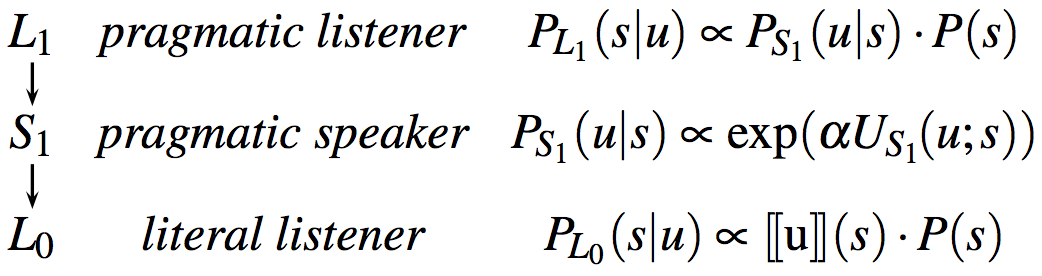
\includegraphics[width=0.5\linewidth]{vanilla-rsa.png}
	\end{center}
	\vspace{-0.3cm}
	\caption{A schematic depiction of a vanilla RSA model \parencite{problang}}
	\label{vanilla-rsa}
\end{figure*}
Putting all the elements together results in the vanilla version of an RSA-model (Fig.~\ref{vanilla-rsa}).
The crucial illustration of the RSA mechanism is the difference between the distributions inferred by $L_0$ and $L_1$ upon observing the same utterance 'blue'. Reasoning about the utterance-generating speaker-model incorporated in $L_1$, while $L_0$ acts according to literal semantics only, is crucial for the pattern of interpretation we observe: $L_1$ infers that the speaker is more likely to mean the blue square, because if she had meant the blue circle, she could have said 'circle', which would have been less ambiguous, and therefore more informative (Table \ref{rsa-l1}). That is, $L_1$ does not only consider what the speaker actually said, but also what the speaker \emph{could have said}. In contrast, $L_0$ infers equal probabilities of 'blue' meaning 'blue square' or 'blue circle' because the utterance is literally true of both referents (Table \ref{rsa-l0}). Crucially, this pattern predicted by the RSA-model is well in line with rational behaviour of humans gathered empirically in such reference game scenarios, confirming that human interlocutors make use of more than just the literal semantics of their words when communicating \parencite{frank2012predicting, problang}.

%Having set the basic building blocks of RSA models, some more sophisticated features of RSA relevant for modelling adjectives should be mentioned. 

%note that these exist as part of L1's reasoning \parencite{lassiter2017adjectival}
\section{Previous RSA Models of Gradable Adjectives}
In this section, previous RSA models of gradable adjectives are discussed; they showed that RSA is a flexible tool suitable to integrate more complex pragmatic reasoning required for interpreting vague expressions.
%threshold semantics, where the threshold is probabilistically inferred \parencite{lassiter2017adjectival} for a given comparison class.

\textcite{lassiter2013context} first provided a model of gradable adjective interpretation within the RSA-framework, showing that pragmatic reasoning can capture their meaning via inference over the latent standard of comparison variable $\theta$ underlying the vague semantics (s. Chapter \ref{chapter02}). %Importantly, probabilistic reasoning provides tools to capture uncertainty over certain aspects of the message, in this particular case - the speaker’s intended meaning of the adjectival utterance.  
The proposed model builds upon the standard RSA model with three levels, adding one crucial extension: the pragmatic listener $L_1$ jointly infers the value of the threshold $\theta$ along with the state of the world $s$ (i.e., the degree to which a referent possesses the property described by the adjective):
\begin{equation}
P_{L_1} (s, \theta \mid u) \propto P_{S_1} (u \mid s, \theta) \times P (s) \times P(\theta)
\end{equation} 

The model formalized literal meaning of gradable adjectives in terms of degree-semantics, assuming that the lexical entry of the adjective specifies the underlying scale and its polarity (cf. Chapter~\ref{chapter02}):
\begin{equation}
\llbracket u \rrbracket_{\theta} (s) = s > \theta
\end{equation}
However, the literal meaning of the adjective by itself is underspecified - it depends on the pragmatically recovered threshold $\theta$, which in turn depends on the comparison class used in the particular context; yet, like vanilla RSA the model is anchored in the literal interpretation of the adjective applied to a referent at the level of $L_0$.  
So in order to allow specifying the $L_0$ which requires computating the truth-value of an utterance for a given state, the authors proposed $L_1$ consider all possible assignments of the \emph{lifted} latent variable value $\theta$, given a prior over that variable $P(\theta)$. A uniform $P(\theta)$ encoded that a priori any property degree might qualify for being described by the adjective. Crucially, the state prior $P(s)$ encoded prior knowledge about \emph{likely property degrees for a specific comparison class} which the referent might have. For instance, the difference in the meanings of \emph{big} in 'big for a tree' and 'big for a pug' would be encoded in different priors over the likely properties of the respective referents. It is common practice to quantify this prior knowledge empirically via prior elicitation experiments \parencite{problang}.

The assumed $\theta$ values are then iteratively passed down through the model. Given a particular value, the speaker-model can be specified:
\begin{equation}
	P_{S_1} (u \mid s, \theta) \propto exp(\alpha \: log (P_{L_0} (s \mid u, \theta) - C(u)) )
\end{equation}	

Then, in contrast to $L_1$ who is uncertain about $\theta$, $L_0$ interprets the utterance literally, so she gets $\theta$ passed down and infers the state distribution consistent with this particular $\theta$ assignment and the observed adjective $u$:
\begin{equation}
P_{L_0} (s \mid u, \theta) = P_{L_0} (s \mid \llbracket u \rrbracket ^\theta = 1 ) \propto \llbracket u \rrbracket ^\theta (s) \times P(s)
\end{equation}

So putting all the layers together, $L_1$ can compute a joint posterior distribution over all possible combinations of states and values of the latent threshold $\theta$ lifted to the level of the pragmatic listener. Notably, \textcite{lassiter2013context} assumed the relevant comparison class to be supplied to the listener, such that she was uncertain only about the standard of comparison. Yet as discussed in chapters \ref{chapter02}-\ref{chapter03} and shown empirically in Chapter \ref{chapter04}, listeners flexibly reason about the intended comparison class because there might be multiple a priori plausible options in absence of an explicit \emph{for}-phrase.

\textcite{tessler2017warm} introduced an RSA-model of gradable adjectives accounting for flexible reasoning about the relevant comparison class via world knowledge (the rationale and behavioural experiments of this study are described in detail in Section~\ref{2.4.}). In particular, in the proposed model the listener is not only uncertain about the standard of comparison $\theta$, but also about the specificity of the relevant comparison class $c$ (superordinate~vs.~subordinate category of the referent), given prior knowledge about typical property distributions in each category. That is, listeners were assumed to know the a priori probability that an adjective could felicitously apply to a referent given its category, assuming a specific comparison class; they used this knowledge to infer the intended comparison class upon hearing a simple adjectival utterance $u$ of the form '\emph{PRON} is \emph{ADJ}' said of a referent whose \emph{subordinate category was known to the listener}.
Similarly to the model proposed by \textcite{lassiter2013context}, the pragmatic listener iterated over all possible value assignments of the lifted $\theta$ variable when reasoning about the utterance-generating process, to jointly infer the property degree $s$, the threshold $\theta$ and the relevant comparison class $c$, given the utterance $u$:
\begin{equation}
P_{L_1}(s, \theta, c \mid u) \propto P_{S_1} ( u \mid s, \theta, c) \times P(s \mid c_{sub}) \times P(c) \times P(\theta)
\end{equation} 
That is, the listener reasoned about how a rational speaker $P_{S_1}$ would behave in order to communicate a specific property, given a comparison class and a threshold, together with their prior knowledge about what property degrees are plausible given the subordinate category $P(s \mid c _{sub})$ the referent belongs to, and their prior beliefs $P(c)$ about which comparison class categories are likely to be used and what properties are likely to qualify for applying the adjective ($P(\theta)$). Accordingly, the speaker-model $P_{S_1}( u \mid s, \theta, c)$ can be specified assuming particular values of the property, the comparison class and the threshold:
\begin{equation}
P_{S_1}( u \mid s, \theta, c) \propto exp(\alpha \: log P_{L_0} (s \mid u, \theta, c))
\end{equation}

The $L_0$ again specifies a literal listener who interprets the adjective $u$ according to its literal semantics, assuming a particular comparison class $c$ and $\theta$:
\begin{equation}
P_{L_0}(s \mid u, \theta, c) \propto \llbracket u \rrbracket_{\theta} (s) \times P( s \mid c)
\end{equation}  
Importantly, $L_0$ now samples states according to a prior $P(s|c)$ specified by the received comparison class $c$, which integrates the comparison class into the literal semantics. 

Since the predictions of this model strongly depend on prior world knowledge, it is important how the property priors given different comparison classes are specified. \textcite{tessler2017warm} fixed superordinate property distributions as $\mathcal{N} (0, 1)$ and subordinate property distributions as $\mathcal{N}(\mu_{sub}, \sigma_{sub})$, inferring the paramters of subordinate distributions from experimental data. The comparison class prior $P(c)$ was approxiamted as empirical Google WebGram frequencies of usage of the respective comparison class labels. 

\textcite{tessler2017warm} showed that the model captures human inferences discussed in Section \ref{2.4.} very well, confirming the role of world knowledge for comparison class inference. 
% potential spot to integrate Dan Yurovsky's work 
However, this model only considered the effect of world knowledge on comparison class inference, and focused on interpretation of simple underspecified utterances of the form 'He is tall'. In the following section, a further extension of previous RSA models is proposed, which accounts for more complex sentences containing a noun and integrates more sophisticated reasoning about several effects contributing to comparison class inference.  

\section{Reference and Predication in RSA}
This section outlines a novel RSA model formalizing the reference-predication trade-off hypothesis.

First, let's recall the reference-predication trade-off hypothesis: it posits that speakers pursue particular \emph{informational goals --- reference} and \emph{predication} --- when crafting their utterances. These informational goals are realized by the speaker syntactically via different positions of the noun: the noun is more likely to contribute to reference when appearing in the sentence subject, especially when combining with the deictic "that", but less likely to do so when appearing in the predicate. Hence, nouns appearing in the subject can be potentially \emph{explained away} by their utility in reference, while nouns appearing in the predicate  are less likely to contribute to reference and therefore more likely to contribute to predication --- i.e., constrain the comparison class. Listeners, in turn, reason about these speaker goals when interpreting the observed utterance.  
Therefore, the degree to which the noun of the sentence constrains the comparison class --- i.e., serves predication --- trades off with its utility in reference. 

\subsection{Questions Under Discussion in RSA}
\label{rsa-qud}
Reasoning about particular informational, or conversational, goals is closely related to basic assumptions made in RSA.
As described in Section~\ref{intro-rsa}, the speaker is assumed to be a rational agent producing utterances of optimal utility with respect to some specific \emph{conversational goal} determined by discourse, also called \emph{question under discussion (QUD)}  \parencite{lassiter2017adjectival, roberts2012information}. The communication is structured so as to maximize the probability that the listener infers the intended \emph{answer to this QUD}. In the vanilla example introduced in Section~\ref{intro-rsa}, the QUD was to determine the intended referent, and the intended answer was 'blue square'. From this perspective, interlocutors' contributions to discourse are \emph{relevant} if and only if they contribute to answering the question under discussion \parencite{roberts2012information}. Note that such questions under discussions might indeed be realized by specific speech acts, but do not have to be - they often remain implicit, and resemble questions rather formally in that they proffer the set of relevant alternatives interlocutors commit to addressing. Yet, interlocutors are fascinatingly good at determining the QUD pragmatically so as to functionally organize their communication around the QUD; they might do so by using different strategies, one prominent strategy in English being to make use of focus \parencite{roberts2012information, krifka2008basic}. But they might also employ other strategies, like choosing particular syntactic structures over others --- e.g., as proposed by the reference-predication trade-off hypothesis.  

From a semantic perspective, utterances then might have several dimensions of interpretation, each dimension corresponding to the interpretation of the utterance satisfying a distinct communicative goal, or answering a distinct QUD. This idea was first formlazed within the RSA-framework by \textcite{kao2014nonliteral}, applied to hyperbolic and pragmatic halo effects in interpretation of number words. The crucial novelty they introduced was listener uncertainty about the relevant QUD along with the multi-dimensional literal meaning of utterances, where each dimension satisfied a distinct potential QUD. The speaker in this model thus chose utterances optimally conveying her particular intended QUD \parencite{kao2014nonliteral}. %\pt{add formulas if necessary}

Another approach to formalizing multiple conversational goals was taken by \textcite{yoon2016talking} who proposed a model of polite language. The authors noted that although politeness phenomena were argued to violate basic cooperative principles of quality, they can be explained as produced by rational interlocutors pursuing not only the goal of informativeness, but simultaneously also a \emph{social goal} \parencite[cf.][]{brown1987politeness, yoon2016talking}. That is, by using polite sentences speakers strive to trade off being informative and saving the listener's self-image, or \emph{face}. Omitting here the details of how exactly this social goal was formalized, the authors proposed a model wherein the speaker tried to balance the utility of an utterance as simulatneously achieving the social goal and the goal of being maximally informative. She did so by maximizing a global utility function, which consisted of a weighted combination of these two utility sub-functions. The pragmatic listener then reasoned about the exact weighting of these two goals \parencite{yoon2016talking}. 

Yet the majority of RSA models usually assume that speakers address one particular conversational goal. The listener might be uncertain about it, as in case of QUD-models, but mostly models might just addressed one pre-defined aspect of communication, i.e., one QUD \parencite[see][for an excellent overview of various RSA models]{problang}. 

This work has argued that interlocutors at least consider multiple informational goals (i.e., QUDs) that might be addressed within the same utterance containing a noun and a gradable adjective, reasoning how different parts of the utterance might probabilistically contribute to achieving each of the goals. Therefore, in the following a model is proposed which attempts to formalize the reference-predication hypothesis. It treats speakers' choice of utterances as \emph{incremental}, where the subject is chosen so as to establish reference, and the predicate is chosen to convey the comparison class --- and so one utterance is optimized to fulfil multiple QUDs. 

\subsection{Refpred-RSA Model}
\label{refpred-rsa}
In the following, the basic structure of the novel reference-predication RSA-model is presented. %Then, different potential representations of the speaker-utility function integrated in that basic structure are presented and discussed.
Then, model predictions are qualitatively compared to the results of the Comparison Class Inference Experiment (s. Section \ref{experiment3}). It will be shown that minimal extensions to existing models result in accurate predictions about the identity of an unknown referent, its property, and crucially, the intended comparison class. 
%It will be shown that minimal extensions to existing models result in accurate predictions about identity of an unknown referent and its property, but predictions about the lifted comparison-class variables are limited if assuming the representation used by \textcite{tessler2017warm}. 
The model is intended to predict comparsion class inferences drawn from sentences differing in the type of the noun (basic~vs.~subordinate referent label) and its position (subject~vs.~predicate), investigated empirically in Experiment 3 (s. Section~\ref{experiment3}). The anaphoric "one" condition is disregared, because it was rather an experimental sanity-check condition. This model is inspired by previous gradable adjective interpretation models: The representation of adjectival meaning is represented in terms of threshold semantics, similarly to the proposal by \textcite{lassiter2013context}; the comparison class representation is inspired by the model by \textcite{tessler2017warm}.

In the basic model, upon hearing an utterance of the form "That N is ADJ" or "That's a ADJ N" the pragmatic listener tries to resolve his uncertainty about the specific member of the context the speaker is referring to, its size and the comparison class intended by the speaker. As a first approximation, driven by present experimental results and previous work by \textcite{tessler2017warm}, it is assumed that the potential comparison class is either the subordinate or the basic-level category of that referent. The potential referent might be one of the members of the perceptual context (i.e., basic-level or subordinate context), though the listener knows the subordinate category of the intended referent.\footnote{Note that this representation might not fully correspond to experimental set-up: The intended referents of the sentences were made salient by presenting them in a picture separate from the context. However, if anything, this representation might be seen as more conservative than the empirical set-up, because it puts a generally higher referential pressure on the speaker.} Therefore, the listener is assumed to know the subordinate categories of all possible referents, which informs their potential sizes.
Formally, the listener infers the comparison class $cc$, the referent $r$ and its size $s$ given an utterance $u$ and a perceptual context $C$:
\begin{equation}
P_{L_1} (r, s, cc \mid u, C) \propto P_{S_1} (u, cc \mid s, r, C) \times P(r, s \mid C, cc_{r\_sub}) 
\end{equation}
That is, the listener infers the referent, its size and the comparison class by reasoning about how a speaker would behave in order to communicate a particular referent and its size in context, in addition to his prior knowledge about different subordinate categories. All referents in context are treated as equally likely to be discussed, but more sophisticated models might upgrade the prior to incorporate perceptual salience, for instance for referents standing out with respect to their size. 

Importantly, rather than representing the comparison class as a variable lifted to the level of the pragamtic listener $L_1$ \parencite[as proposed by][]{tessler2017warm}, the intended comparison class influencing the resolution of the adjective is represented as a concious \emph{lexical choice, or a local enrichment} made by the speaker \parencite[e.g., discussed by][]{chierchia2012grammatical, problang}. So while the pragmatic listener in \textcite{tessler2017warm} assumes that the speaker has a fixed meaning of the adjective (e.g., "big for a dog" or "big for a Great Dane") which the listener is uncertain about, in the current model the pragmatic listener reasons about a speaker who might \emph{variably} choose her intended adjective meaning \parencite[cf.][]{problang}. 
This was proposed in prior work arguing that pragmatic enrichments might already take place at subsentential --- i.e., lexical --- level, such that the speaker chooses to convey one of grammatically supplied local phrase readings with her utterance \parencite[for instance, applied to scalar implicatures by][]{chierchia2012grammatical}. In the current case, the speaker can choose between the subordinate and basic-level comparison class relative to which the adjective will be interpreted, in addition to the option to use a predicative noun as the comparison class. 
%\pt{add some explanations/background on what local enrichment is from Chierchia } 

So the speaker determines an \emph{optimal utterance and comparison class} in order to communicate a referent and its size, given the adjective she wants to use and the context, by optimizing the speaker-utility function $U$:
\begin{equation}
P_{S_1} (u, cc \mid s, r, C)  \propto exp(\alpha \: U_{S_1}(u; s; r; cc; C) \times P(cc) \times P(u)) 
\end{equation}
The cost of producing uterances $C(u)$ is assumed to be uniform over all possible utterances and is therefore neglected. The optimality parameter $\alpha$ was arbitrarily set to a generic value of 3 for the simulations presented below. The utterance utility $U$ is combined with the speaker's prior $P(cc)$ over possible comparison classes (a uniform distribution over basic~vs.~subordinate referent categories) and possible utterances ($P(u)$).
As mentioned above, one novel aspect of this model is that the speaker constructs the utterance incrementally: she considers the subject and the predicate separately, choosing uniformly at random where to put the noun. Since two potential comparison classes are considered in this model, the possible noun options are the subordinate or the basic-level label of the intended referent. That is, the speaker may put the noun in the subject, so the sentence would match the experimental subject-N condition. The predicate is then a bare adjective ("big" or "small"). Alternatively, the speaker may put the noun in the predicate, directly modified by the adjective; the subject is then the bare deictic "that", resulting in the predicate-N experimental condition. Furthermore, the speaker may choose the adjective to convey one of the two possible comparison classes, since she infers the optimal comparison class: for instance, she might choose "big" to mean "big for a dog" or "big for a Great Dane", irrespective of the noun position. This results in eight possible utterances the speaker considers (noun position $\times$ noun type $\times$ comparison class).  

In contrast to models including several QUDs reviewed in Section \ref{rsa-qud}, for this case-study one might posit that speakers a priori pursue both the goal of reference and the foal of predication. Therefore, most intuitively, the speaker utility can be represented jointly with respect to two-dimensional states of the world consisting of a referent and a size dimension she wishes to communicate (but see Appendix \ref{appendix} for alternative formalizations, following those discussed in Section \ref{rsa-qud}). Conceptually, when communicating the referent she addresses the reference-QUD, when communicating the size --- the predication-QUD, respectively. According to the operationalization assumed in this work, the subject part of the utterance is optimized for transmitting reference, the predicate for predication: 
\begin{equation}
\label{model1}
U_{S_1} (u; r; s; cc; C) = log \: L_0 (s, r \mid u, C, cc) 
\end{equation}
In line with basic RSA mechanisms, the speaker utility is grounded in a listeral listener $L_0$ whom the speaker reasons about when choosing the utterance and the comparison class. 
$L_0$ then interprets the utterance chosen by $S_1$ according to its literal meaning, considering the subject as establishing reference, and the predicate as communicating the size of the referent. 
That is, $L_0$ returns a joint distribution over referents and over properties from the context for which the utterance subject is true, and which are possible under the comparison class and the adjective: %If the predicate contains a noun, that noun is taken as the comparison class. If the predicate is a bare adjective, the comparison class variable lifted to the level of $L_1$ passed down provides the comparison class \parencite{tessler2017warm}. 
\begin{equation}
P_{L_0} (r, s \mid u, cc, C) \propto \llbracket u_{Subj} \rrbracket (r)  \times  \llbracket u_{Pred} \rrbracket_{\theta} (s) \times P(r, s \mid C, cc) \times P(\theta)
\end{equation}
The state prior $P(r, s \mid C, cc)$ represents the literal listener's prior beliefs about possible referents and sizes; crucially, the possible sizes now depend on the explicit comparison class $cc$ or the utterance $u$ passed to $L_0$ rather than on the subordinate category of a sampled referent (as for $L_1$). Critically, the reference-predication hypothesis posits that listeners might consider nouns appearing in the predicate as the comparison class; therefore, the literal listener probabilistically considers the noun to be the comparison class, when it is observed in the predicate (taking uniformaly at random the noun or the comparison class $cc$). This provides a hook for representing the effect of a comparison class: for example, intuitively, the distribution of sizes that would count as \emph{big for a Great Dane} is a priori different from the distribution of sizes that would count as \emph{big for dogs}. 
These size priors $P(cc)$ are represented by Gaussian distributions relative to particular comparison classes, \textcite[as proposed by][]{tessler2017warm}. Since this work is concerned with qualitative predictions only, the priors representing properties of different classes are set to $\mathcal{N}(\mu = 0, \sigma = 1)$ for the basic-level comparison class, $\mathcal{N}(\mu = -1, \sigma = 0.5)$ for small-subordinate, $\mathcal{N}(\mu = 0, \sigma = 0.5)$ for medium-subordinate and $\mathcal{N}(\mu = 1, \sigma = 0.5)$ for large-subordinate comparison classes (Fig.~\ref{model1-priors}). 
Furthermore, the inference over the threshold of comparison $\theta$ is moved to the level of $L_0$ for better computational tractability, different from the original proposal by \textcite{lassiter2013context}.
\begin{figure*}[t]
	\begin{center}
		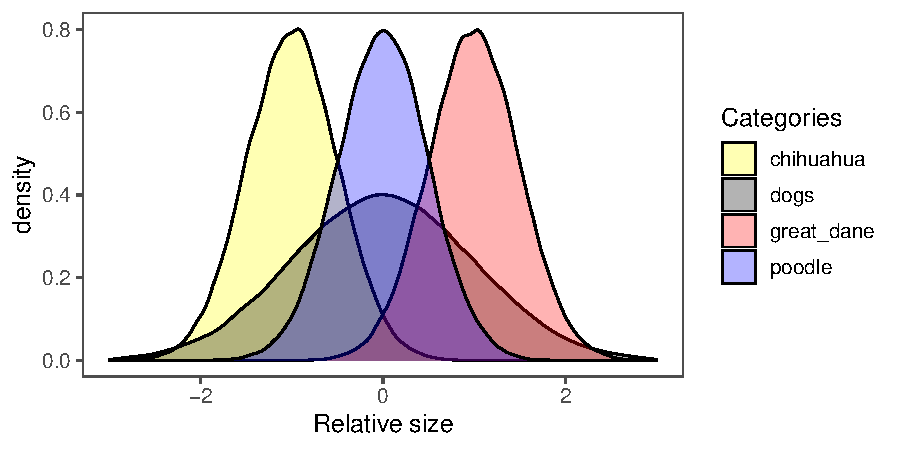
\includegraphics[width=0.7\linewidth]{refpred-RSA_priors.pdf}
	\end{center}
	\vspace{-0.3cm}
	\caption{Hypothetical prior size distributions over a basic-level, a small-subordinate, a medium-subordinate and a large-subordinate category. These distributions were used for qualitative tests of the refpred-RSA model.}
	\label{model1-priors}
\end{figure*}

Since the literal listener infers states consistent with the literal meaning of utterances, the representation of literal semantics of the utterance she observes is a crucial component of the model. This model employs classic Boolean semantics common in RSA models \parencite{montague1973proper}. For the meaning computation, the utterance is split into subject and predicate, and each component is evaluated with respect to one goal (reference or predication, respectively); an utterance is assumed to be true of a state if and only if both components are true.  When computing the meaning of the subject, the bare deictic 'that' and the basic-level nouns are assumed to be true of any member of the context, while subordinate labels only apply to respective category members. The referential utility of the subject is therefore formalized as in the vanilla RSA model (s. Section \ref{intro-rsa}). The meaning of the predicate is computed in terms of threshold semantics, as first proposed by \textcite{lassiter2013context}: 
\begin{equation}
\llbracket u \rrbracket (s, r) = \llbracket u_{Subj} \rrbracket (r) \land \llbracket u_{Pred} \rrbracket_{\theta} (s) = \llbracket u_{Subj} \rrbracket (r) \land \theta > s
\end{equation}
%\pt{Predictions of the different models / conceptual differences / discussion and comparison to E3; potentially move a part to Appendix}
  
So putting all these elements together, the proposed model formalizes a pragmatic listener inferring an intended referent in context, its size and the intended comparison class upon observing a sentence containing a noun and an adjective:
\begin{gather*}
	L_1 (r, s, cc \mid u, C) \propto P_{S_1} (u, cc \mid s, r, C) \times P(r, s \mid C, cc_{r\_sub}) \\
	S_1 (u, cc \mid s, r, C)  \propto exp(\alpha \: log \: L_0 (s, r \mid u, C, cc) \times P(cc) \times P(u)) \\
	L_0 (r, s \mid u, cc, C) \propto \llbracket u_{Subj} \rrbracket (r)  \times  \llbracket u_{Pred} \rrbracket_{\theta} (s) \times P(r, s \mid C, cc) \times P(\theta)
\end{gather*}
 
\begin{figure*}[t]
 	\begin{center}
 		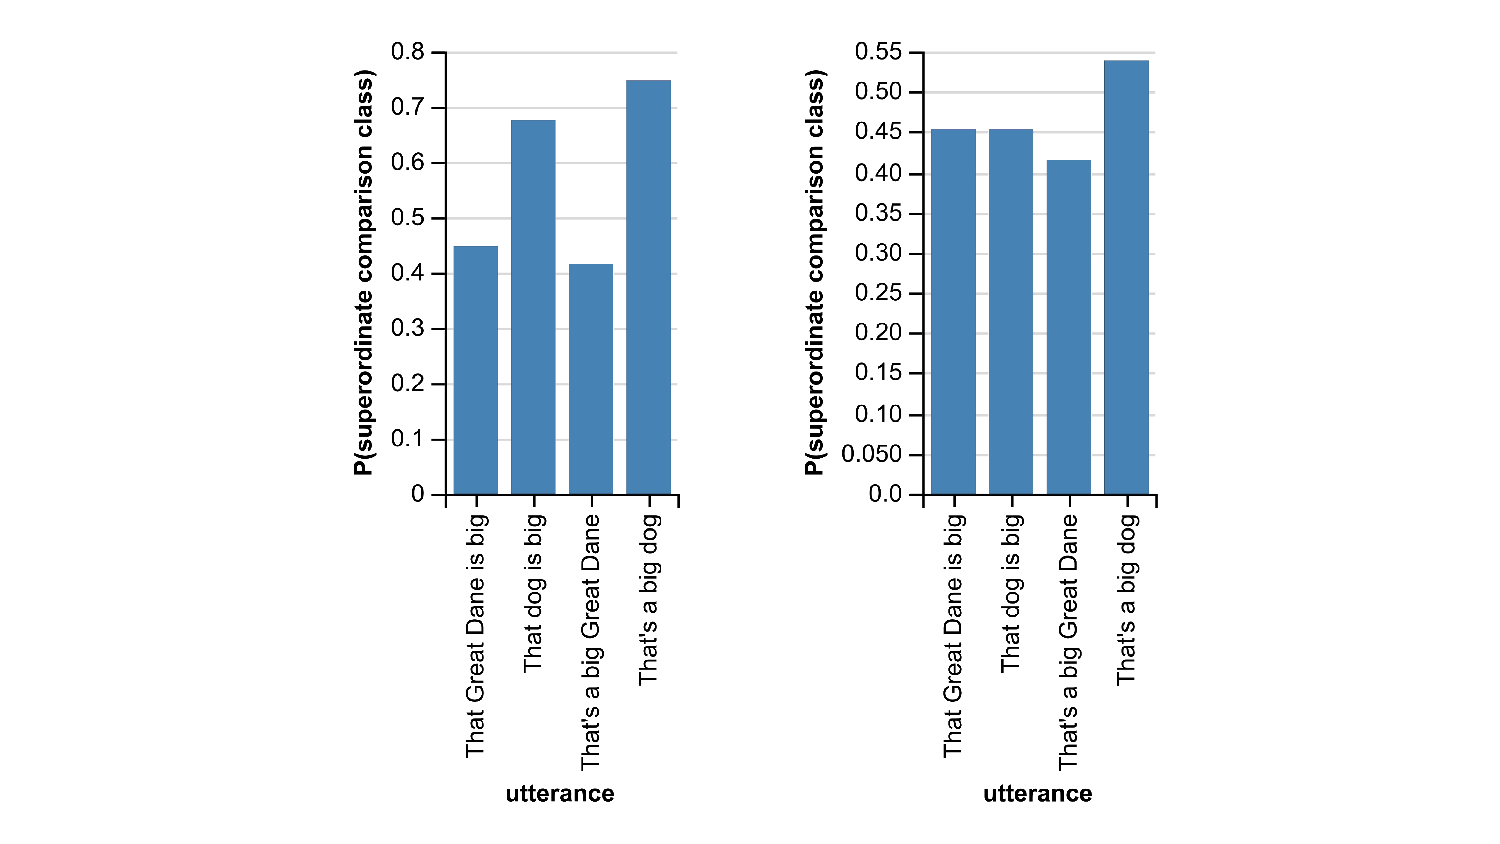
\includegraphics[width=\linewidth]{model1-cc-posteriors.pdf}
 	\end{center}
 	\vspace{-0.3cm}
 	\caption{Qualitative predictions made by the refpred-RSA model: Pragmatic listener inferences are plotted in terms of the probability to use the basic-level comparison class (i.e., "big for a dog"), given utterances differing in the noun and its position, presented in a basic-level context (left)~vs.~subordinate context (right). Qualitatively, the crucial noun$\times$syntax interaction can be observed. Note the different y-axis scaling.}
 	\label{model1-cc-results}
 \end{figure*}
In order to investigate whether the qualitative predictions of this model capture the essence of predictions made by the reference-predication hypothesis, supported by the data observed in Experiment 3, the model was implemented using the probabilistic programming language WebPPL \parencite{dippl}. The pragmatic listener model was then tested on example sentences matching critical conditions from Experiment 3 (s. Section \ref{experiment3}). Most importantly, the model should capture the contrast in comparison classes inferred from subordinate-noun sentences differing in the position of the noun, distinct from basic-level noun sentences.

Figure \ref{model1-cc-results} (left) shows the proportion of basic-level comparison classes (i.e., "big for a dog") the model predicts upon observing example utterances containing the nouns "dog"~vs.~"Great Dane", appearing in the subject~vs.~predicate position, given a basic-level context. 
Visually, the critical contrasts can be observed: the model predicts that the basic-level comparison class is less likely given the utterance "That's a big Great Dane", relative to "That Great Dane is big". Furthermore, the model captures that the basic-level comparison class is generally less likely if the utterance contains a subordinate noun. Finally, the pragmatic listener infers more basic-level comparison classes given the utterance "That's a big dog" than the utterance "That dog is big", which is generally consistent with reference-predication hypothesis predictions, though was not observed in Experiment 3 due to a ceiling effect in the basic-level context (s. Figure \ref{cci-results}). 

\begin{figure*}[t]
	\begin{center}
		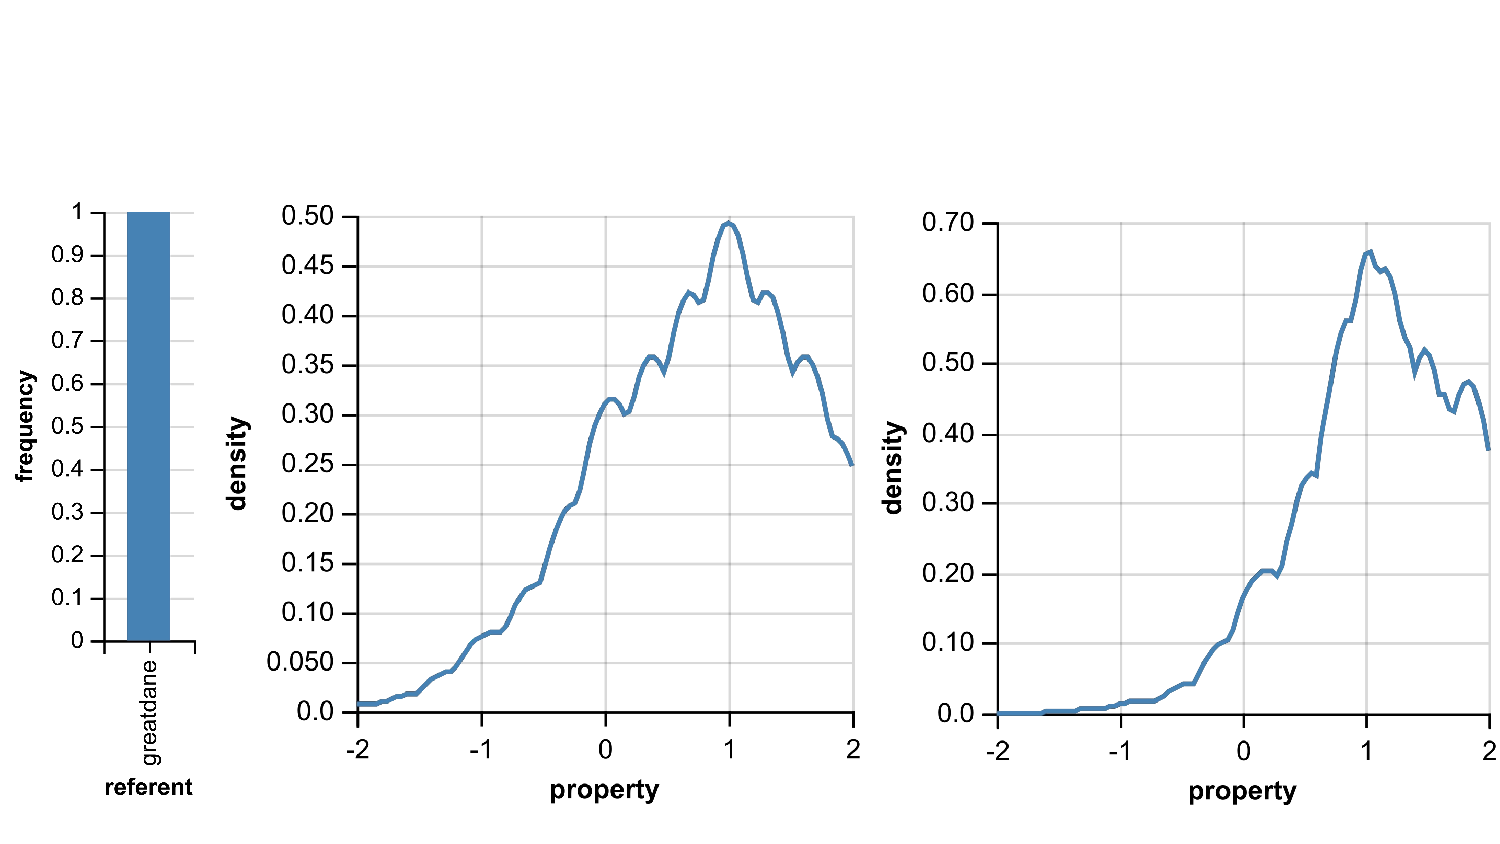
\includegraphics[width=\linewidth]{model1-ref-size-posteriors.pdf}
	\end{center}
	\vspace{-0.3cm}
	\caption{Qualitative predictions made by the refpred-RSA model: Given the utterance "That Great Dane is big", the pragmatic listener infers a large-subordinate size distribution (middle) and is certain that the referent is a Great Dane (left). Given the utterance "That's a big Great Dane", the pragmatic listener shifts her size distribution even more towards large size values (right), and is again certain about the referent (left).}
	\label{model1-ref-size-results}
\end{figure*}
\begin{figure*}[h]
	\begin{center}
		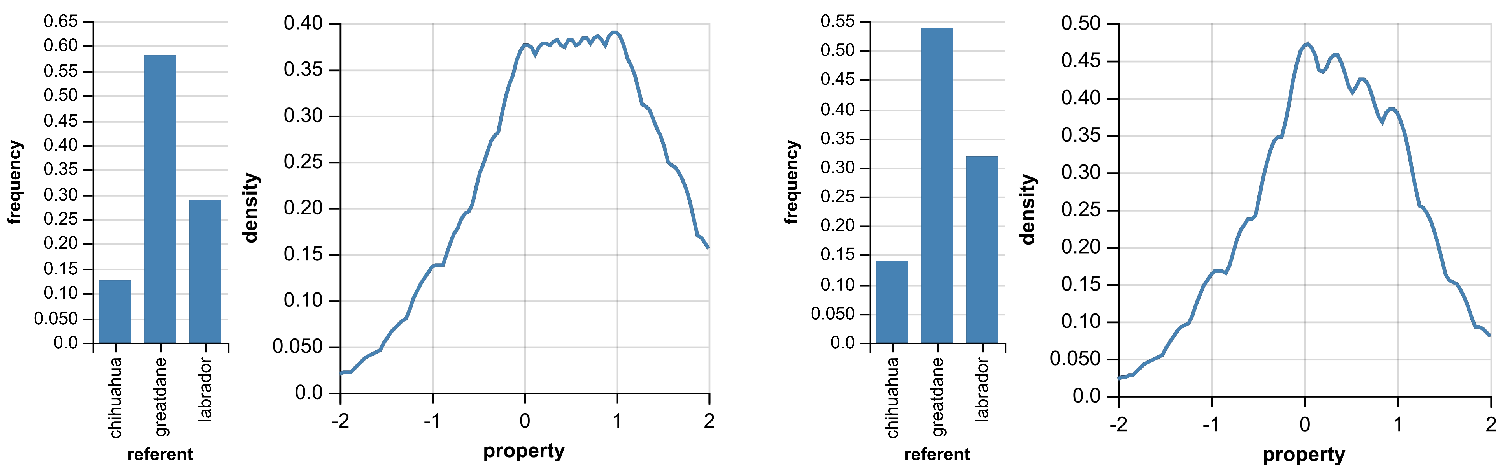
\includegraphics[width=\linewidth]{model1-basicN-basicC-crop.pdf}
	\end{center}
	\vspace{-0.3cm}
	\caption{Qualitative predictions made by the refpred-RSA model given the utterances with a basic level noun in basic-level context (from left to right): distribution over referents, distribution over sizes inferred from "That dog is big" (subject N); distribution over referents, distribution over sizes inferred from "That's a big dog".}
	\label{model1-basicN-basicC}
\end{figure*}
\begin{figure*}[b]
	\begin{center}
		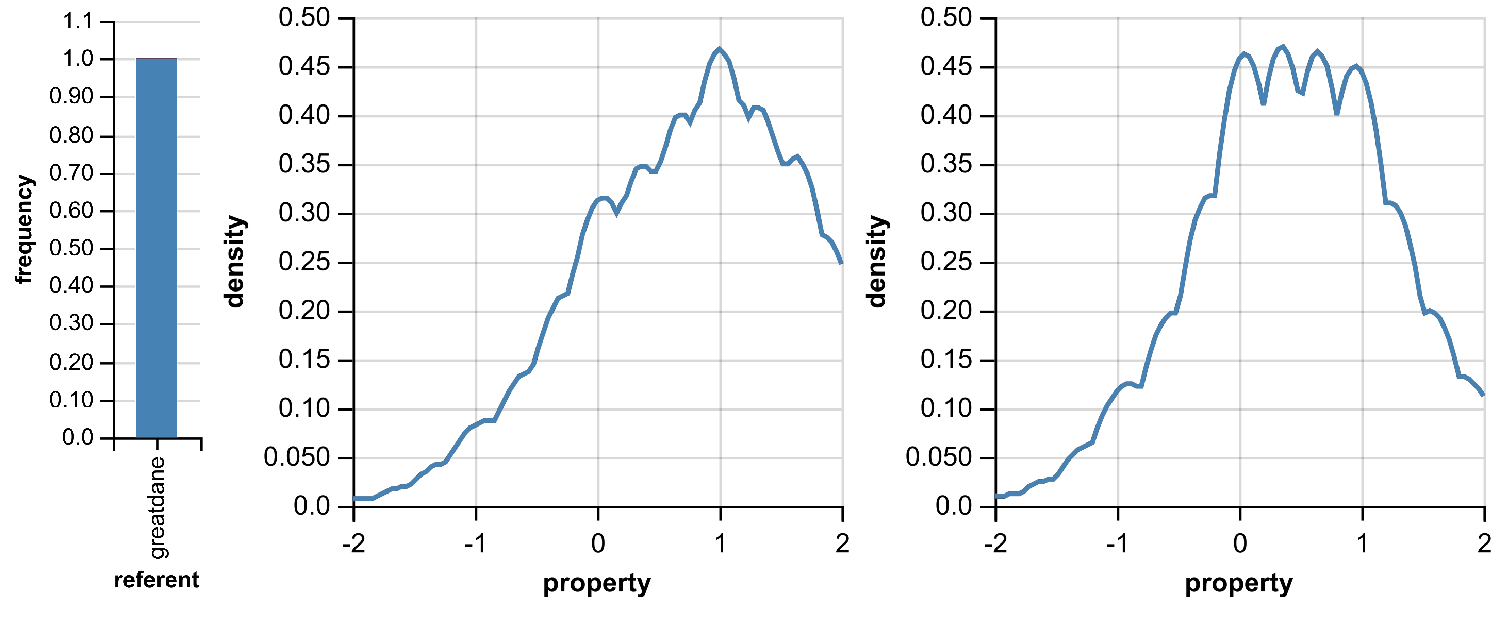
\includegraphics[width=\linewidth]{model1-basicN-subC-crop.pdf}
	\end{center}
	\vspace{-0.3cm}
	\caption{Qualitative predictions made by the refpred-RSA model given the utterances with a basic level noun in subordinate context (from left to right): distribution over referents, distribution over sizes inferred from "That dog is big" (subject N); distribution over sizes inferred from "That's a big dog".}
	\label{model1-basicN-subC}
\end{figure*}

The model performs comparably well given the same utterances in \emph{subordinate} context (Fig.~\ref{model1-cc-results}, right). First, consistent with data observed in Experiment 3, the model captures a grand influence of context: overall, the basic-level comparison class is less likely given the subordinate context than the basic-level context (Fig.~\ref{model1-cc-results}, left~vs.~right). Second, the model captures reasoning about contextual referential utility, rendering both nouns in the subject position equally referentially uninformative. Finally, both nouns in the predicate position are more likely to signal their respective comparison class than in the subject position.

In both contexts, given the critical utterances containing a subordinate noun, the model infers the expected referent and size distributions (Fig.~\ref{model1-ref-size-results}). That is, the inferred referent matches the noun; the inferred size distribution is shifted more strongly towards the subordinate category size values when observing an utterance containing a predicate noun relative to an utterance containing a subject noun. 
When the noun is the basic-level target label, in the basic-level context the pragamtic listener is uncertain about the intended category of the referent (Fig.~\ref{model1-basicN-basicC}). As predicted, the inferred size distributions do not differ qualitatively in the basic-level context across the two sentence frames, but do so in subordinate context: when the noun appears in the predicate, the listener shifts her distribution more towards the basic-level category properties, but infers a more subordinate --- contextually informed --- distribution when the noun is in the subject (Fig.~\ref{model1-basicN-subC}). These results provide further support that the model represents the reference-predication hypothesis well.

In sum, this model formalizes the reference-predication trade-off hypothesis via recursive probabilistic reasoning, representing a pragmatic listener as considering an agent choosing the adjective to convey a particular comparison class. It integrates reasoning about both syntactic and semantic aspects of the utterance and generally captures comparison class inferences observed empirically, driven by the trade-off of the noun utility for different informational goals. It was shown that such a complex inferential hypothesis can be qualitatively explained by minimally extending existing generic Rational Speech Act tools. To the best of our knowledge, this is the first attempt to formalize reasoning about both meaning and structure of an utterance within the RSA framework,  contributing to both creating more accurate gradable adjective interpretation models and extending the scope of RSA models. 


\chapter{Discussion}
\label{chapter06}
Humans use language across infinitely many different situations. By the age of two infants already learn that the same words might be used in different contexts and convey different meanings, allowing for fascinatingly versatile and efficient language use \parencite{Mintz2002, ebeling1994children}. 
Relative gradable adjectives are one, but not the only, example of natural language expressions whose meaning greatly depends on context (e.g., next to \textcite[indexicals][]{braun2017}; or \textcite[anaphoras][]{goldberg2017one}, inter alia). Yet speakers almost never establish explicitly which aspects of context are relevant and leave it to the listener to pragmatically reconstruct. Interpreting gradable adjectives requires establishing a context-dependent comparison class by inferring to what aspects of (non-)linguistic context the referent is being compared. This task is relevant for the interpretation of a number of other expressions, as comparison classes are also employed when understanding other kinds of context-sensitive language like quantifiers \parencite[e.g., "John ate \emph{many} of hot dogs",][]{scholler2017semantic} or generics \parencite[e.g., "Dogs are friendly" \emph{[relative to other animals]},][]{tessler2019language}. 

This thesis investigated the interpretation of relative gradable adjectives as a case-study of context-sensitive language and attempted to contribute to understanding how exactly listeners might establish relevant comparison classes. 
Standard literature on gradable adjective semantics suggests that the comparison class might be supplied by the noun the adjective combines with; however, this work argued that purely compositional accounts might be too rigid to explain the flexible use of gradable adjectives across contexts. Furthermore, even when allowing that relevant contextual aspects supply the comparison class, much of the research on gradable adjective semantics eschewed the question how exactly a comparison class might be determined contextually, instead focusing on its integration into compositional semantics \parencite{Kennedy2007, kennedy2012, Kamp1975, Cresswell1976, Solt2009}. 
Therefore, this work outlined a novel functional hypothesis regarding the role a noun might have for comparison class inference in addition to contextual cues --- namely the \emph{reference-predication trade-off hypothesis}. The quintessential prediction derived from this hypothesis is that listeners are less likely to take the noun as a cue towards the comparison class when the noun can be expained away as intended for the informational goal of reference, operationalized via the syntactic position of the noun the adjective combines with. Specifically, nouns appearing in the subject of the sentence can be explained by their utility in reference and are therefore less likely to set the comparison class, while nouns in the predicate are less likely to be referential and are therefore more likely to constrain the comparison class.

Four experiments were conducted to investigate this hypothesis. Experiment 1 showed that participants appreciably disprefer sentences where a subordinate noun appeared in the predicate compared to sentences with a basic-level noun in the predicate as describing a normal-sized referent, indicating that participants preferred sentences with a more felicitous comparison class label in the predicate. Experiment 2 revealed that participants flexibly adjust their noun choices given different syntactic frames in a free-production setting, producing more basic-level nouns in the predicate than in the subject position. Experiment 3 indicated that participants are highly sensitive to the perceptual context of the utterance, to the noun of the utterance and to its syntactic position when asked to paraphrase the comparison class, trading-off the noun's utility in reference and predication when reasoning about its cue strength towards the comparison class. Finally, a pilot study for Experiment 4 showed that reasoning about informational goals accomplished by the noun is indeed the driver behind participants' reasoning about comparison classes, as opposed to mere presence of direct syntactic modification of the noun by the adjective. % Participants were more likely to infer the subordinate comparison class from directly modified subordinate nouns appearing in the predicate than in the subject position. 
Together, these experiments provide converging evidence that humans use information structure when reasoning about the comparison class, consistent with the reference-predication trade-off hypothesis. 

Studies presented here investigated the role of perceptual context, noun type and its syntactic position on comparison class inferences; while covering major cues towards the comparison class, the particular operationalization of the hypothesis via syntactic manipulation between subject and predicate position of the noun invites investigation of further aspects in future work. For one, all experiments presented critical utterances in written form, yet one other factor that is closely related to information structure is \emph{prosody} \parencite{krifka2008basic}. Prosody might provide a strategy to both structure information and construct new content: for instance, prosody realising focus of a sentence might indicate the presence of relevant alternatives for the focused expression, convey the topic of the utterance or emphasize new information \parencite{krifka2008basic, selkirk1995sentence}. 
Applied to sentences used in present studies, uttering the sentence "That Great Dane is \textsc{big}" (\textsc{big} being prosodically prominent) might convey that the speaker deems the size of this referent particularly noteworthy and therefore shifts the communicative goal towards predication - a perfectly reasonable scenario where the Great Dane is actually big \emph{for} a Great Dane, making the subordinate subject-noun the comparison class.  Alternatively, the same utterance is imaginable in a situation where someone said "That Great Dane is small" and the speaker replied "No, that Great Dane is \textsc{big}". The latter example goes in the direction of meta-linguistic or predagogical uses of gradable adjectives where the speaker informs the listener about what he considers a viable use of size adjectives given the particular referent. Uttering "That \textsc{Great Dane} is big" might signal that a Great Dane is being contrasted against other categories or referents, highlighting the referential goal of the noun.
Prosodically different readings also seem possible for the predicate-N utterance in different contexts. For instance, saying "\textsc{That}'s a big Great Dane" might contrast a particular referent against other Great Danes; or teach the listener about what the speaker considers a good representative of a big Great Dane. The latter example seems plausible in a context where e.g. other big dogs or Great Danes were previously discussed. Uttering "That's a \textsc{big} Great Dane" again seems to imply meta-linguistic or contrastive intentions, while "That's a big \textsc{Great Dane}" would highlight the category of the referent, relevant in some way for the current communicative goal(s). 
Generally, prosody as a tool for both information packaging and content construction might affect the question under discussion and therefore the informational goal in focus, so effects of prosody on comparison class inferences and their connection to the refernence-predication hypothesis should be addressed in future work \parencite[cf.][]{krifka2008basic}. 

For another, it should be noted that this particular experimental approach was chosen in order to keep a maximally simple and controlled design. So for practical reasons of stimulus presentation only size-adjectives 'big' and 'small' were used; however, the reference-predication trade-off hypothesis is applicable to relative gradable adjectives in general, so further experiments involving other adjectives should be conducted. 
Furthermore, the experiments used stimuli from natural basic-level categories only; salient taxonomic representation of such categories might play a role for listeners' reasoning about potential comparison classes, by providing salient viable alternative comparison categories (i.e., subordinate and basic-level categories, \textcite[cf.][]{rosch1976, tenenbaum2011grow}); there might be potentially relevant psychological differences between natural and articifical concept representations though %have been addressed in the literature
 \parencite{kalish2002gold}. 
Additionally, only one specific (schematic) referent picture per subordinate category was used across experiments; future studies should consider varying the pictures in order to average out potential typicality and nameability effects of the pictures as representations of those categories. Relatively high by-target random intercepts across experiments suggested that targets might have varied in those aspects (e.g., resulting in different propensities of the speakers to use subordinate labels). Running a typicality or nameability rating study on the used categories and pictures might also be useful for eliciting priors for fitting the RSA model quantitatively to observed data \parencite{franke2016does}. %Additionally, the relation of comparison classes to typicality of the target for its basic-level category should be investigated more carefully. 

Furthermore, in order to be able to create maximally symmetric utterances across different contexts and syntactic conditions, the noun phrase in the predicate position was always indefinite, and the subject noun phrase was always definite. If the predicate was definite, the triggered uniqueness presupposition would have been violated, deeming these sentences generally less natural (i.e., saying "That's \emph{the} big Great Dane" would trigger the expectation that there is only one Great Dane, which is not true of contexts used in the experiments) \parencite[cf.][]{syrett2010meaning}. 
For this reason, the definiteness of the noun is perfectly confounded with its position throughout the experiments. Yet utterances with a definite predicate noun could be tested in an appropriate discourse context where there is only one individual denoted by the noun. The reference-predication hypothesis would predict that definite nouns in the predicate might still be more likely to establish the comparison class than subject nouns irrespective of their higher referential value compared to indefinite ones, as long as reference was already established in the subject. 
The hypothesis, however, does not seem to be operationalized by alternative sentences where the subject noun would be indefinite, since indefinite nouns generally do not refer; these sentences might rather interface with generic or meta-linguistic uses of adjectives \parencite{Reboul2001, tessler2019language, barker2002dynamics}. 

Generally, referential pressure was not very high in current experiments. Referential purposes of the noun were mainly communicated through its combination with the deictic and its position in the subject, which might rely on general information-structural expectations (s. Chapter \ref{chapter03}). But the target referent was perceptually highlighted in a separate picture throughout the experiments. The implied contextual referential pressure might be potentially manipulated in further experiments, e.g., by presenting the referent as a non-highlighted member of the context. \pt{idscuss relation between experimental results, between communicative goals , cf. ELM comments}
%Another potential confound - definiteness. \pt{discuss in chapter 6 that deconfounding definiteness from syntactic manipulation should be addresses in future research; keep it maximally symmetric in E1-3; tentative predictions for E4: same distinction for "A prize-winner is a big great dane" vs "A big great dane is a prize-winner"; infelicitous presuppositions for both parts being definite; also discuss connection to plural / generics / predagogical language;}

%Use more adjectives, different pictures, consider typicality effects.  namability effects 
%Investigate referential pressure.
Besides experimental evidence, this work also provides a computational model of the reference-predication hypothesis within the Rational Speech Act framework. The proposed model builds upon and advances beyond previous RSA-models of gradable adjectives by incorporating simultaneous reasoning about general knowledge, lexical and syntactic cues towards the comparison class. This pragmatic listener model infers a potential state of the world (a referent and its size) along with the likely comparison class. In particular, the listener reasons about how a speaker would behave in order to communicate a specific state, also referring to their prior knowledge about likely sizes of different categories. Crucially, the listener assumes that the speaker might variably choose the intended adjective meaning, and therefore the comparison class. 
In addition, the speaker constructs her utterances incrementally by deciding whether to put the noun in the utterance subject or in the predicate, so as to optimally achieve reference with the subject, and predication with the predicate. This representation allows the speaker to achieve two informational goals simulatneously by using one sentence. By using hypothetic fixed priors, qualitative predictions were derived from the model. It was shown that it is a good first formalization of the reference-predication trade-off hypothesis because it captures essential contrasts observed in Experiment 3. Specifically, the pragmatic listener was more likely to take the noun as a cue towards the comparison class when it appeared in the predicate than in the subject, while taking into account referential utility of the noun. In sum, the proposed model provides a first attempt to integrate pragmatic reasoning about both syntax and semantics of an utterance within the Rational Speech Act framework. 
%Representing adjectival meaning as a local enrichment is novel in this adjective model. 

%\pt{Model discussion and criticism, Novel contribution of this model if any.   }
However, the predictions derived from the proposed model were only qualitative. Future work should evaluate its potential to fit the data observed in Experiment 3 quantitatively. To do so, experiments eliciting participants' prior knowledge of relative category sizes could be conducted \parencite{franke2016does}, or the priors could be reconstructed from indirect experimental results relying on the same prior knowledge \parencite[following][]{tessler2017warm}. The free speaker optimality paramter should then also be determined more accurately, e.g., via a maximum a posteriori estimate. %Furthermore, the model represented a higher referential pressure on the speaker than might have been the case in the experimental set-up. 
Furthermore, additional assumptions were made for this model: for one, inference over the standard of comparison value used for computing literal semantics of the adjective was performed by the literal listener. The cognitive plausibility of this adjective meaning representation remains to be investigated. In addition, it was assumed that the listener and the speaker share identical world knowledge about likely sizes for different categories. Incorporating their reasoning about each other's world knowledge in future work would potentially extend this model to account for meta-linguistic uses of gradable adjectives (s. Chapter \ref{chapter02}; \textcite{barker2002dynamics}). Lastly, the model utilized uniform priors over potential referents in context, as well as over potential comparison classes. These assumptions should be revised because referents might differ in their perceptual saliency --- e.g., referents whose size stands out might be generally more likely to be talked about; and comparison class avaliability might vary across different subordinate categories due to namability or typicality effects. One possibility would be to consider corpus frequencies of respective nouns as an approximation of the prior \parencite[following the model by][]{tessler2017warm}, or gather speaker production data. 
More generally, the relation of this formalization to alternative possible models potentially explaining observed data should be addressed in future work. For instance, models of incremental processing might explain general interpretative differences between the subject and the predicate, because the speakers might build their utterance in a way such that sufficient contrastive information is provided at each point in the utterance. Since the adjective generally appeared in the predicate of sentences used in Experiment 3, the subject might be expected to feature referentially more informative nouns than the predicate, because the adjective can only be used for potential target disambiguation later  in subject-N sentences. However, such a model might not account for the results observed in Experiment 4.  
In sum, the proposed lexical enrichment-based model provides the first qualitative example of context-sensitive language interpretation based on unified reasoning about several cues to the intended meaning. The hope is to supply a basis for future investigations of such holistic RSA models applied to various cases of vague expressions, in addition to providing a more sophisticated model of gradable adjective understanding.
%first model to our knowledge incorporating speakers pursuing several communicative goals. 
%Qualitative fit, quantitative fit?

Cues that contribute to adult gradable adjective interpretation also have implications for investigating the developmental course of children's understanding of complex context-sensitive expressions. In particular, already by the age of two infants understand adjectives like 'big' and 'small' and appreciate their context-sensitive nature, sometimes even without adults specifically pointing out the relevant features of context \parencite{Mintz2002, ebeling1994children}. That is, the critical skill to acquire for gradable adjective interpretation is establishing the correct comparison class; while adults often use prepositional \emph{for}-phrases in child-directed speech, such phrases are often indicative of a particular kind of gradable adjective uses - the functional uses (s. Chapter 2, \textcite{ebeling1994children}). Yet when not producing a \emph{for}-phrase, adults might include other syntactic cues towards the comparison class compensating for more ambiguous adjective uses. 

Taking a developmental perspective on the reference-predication hypothesis, one might derive the prediction that adults use nouns in the predicate of sentences more often than in the subject in order to restrict the comparison class more strongly and make the adjective interpretation easier for children. A study was conducted wherein the Providence corpus was annotated with respect to linguistic and environmental cues available to interlocutors using the adjective "big" \parencite{sinelnikova2020}. It provides preliminary evidence that the majority of recorded uses of the adjective "big" were indeed prenominal cases where the modified nominal appears in the predicate of the sentence. 
Moreover, it showed that more modified nouns appeared in the predicate when there were less distractors in the context; when there were more perceptual distractors the modified noun was rather placed in the subject, contributing to reference. Furthermore, it was found that the referent was mostly physically copresent when the noun was used in the predicate, suggesting that reference might have been established by means other than the noun (e.g., pointing). Finally, the intended comparison class for the adjective-nominal predicate constructions was overwhelmingly the normative comparison class (i.e., making reference to implicit general knowledge of the abstract basic-level  category of the referent, mostly denoted by the noun; s. Chapter \ref{chapter02}), indicating that these syntactic frames were used when establishing the comparison class might have been more challenging for the children \parencite{sinelnikova2020}. These preliminary results are consistent with predictions of the reference-predication trade-off hypothesis ---  nouns in the predicate seem to communicate the comparison class of a referent, facilitating understanding of the gradable adjective for kids who might lack other means for pragmatic reasoning like substantial world knowledge. Understanding what kinds of cues are available to children in naturalistic settings might provide a starting point for investigating how they succeed in learning context-sensitive expressions. 

%highlighting the complex relation of an utterance meaning and its form.  Expt / modelling results, new hypothesis% --- investigating human reasoning about this connection provides valuable insights for computational modeling of vague language.

%Sum up uitlity of the reference-predication hypothesis
%copula
%cross-linguistic ideas / reviewer's comments

\section{Conclusion}
% Interface between syntax, semantics and pragmatics. first work to attempt to integrate influences from different sources of information for the comparison class. connection to other context-depending linguistic phenomena; case study for context-dependence and vagueness
To sum up, this thesis took a step towards understanding how interlocutors flexibly use relative gradable adjectives across contexts, by presenting a novel reference-predication trade-off hypothesis of comparison class inference. 
This hypothesis provides a holistic account of how %interlocutors might establish comparison classes when using relative gradable adjectives. It was shown that 
humans might integrate various cues and reason about referential utility of the noun in context, trading it off with the noun's utility in communicating the comparison class. This inferential account is supported by converging evidence from various experiments. Finally, the hypothesis was formalized computationally within the Rational Speech Act framework, utilizing domain-general Bayesian inference tools widely used in models of cognition. % shown that domain-general Bayesian reasoning is a powerful tool suitable to capture this complex inferential account computationally.  %able to account for vague language interpretation. 
 %Integrating evidence from different information sources, 
 It emphasized the sophisticated reasoning at the interface of syntax, semantics and pragmatics that humans perform in order to make clear use vague language. 
Through the lense of reference and predication, this work highlighted a topic of broad interest to cognitive science --- namely the complex interaction between intentions and informational goals in communication, and the factors shaping this relationship.
%This work highlighted 
 %establish comparison classes. %This case-study of vague language provides a fascinating example for how humans can accomplish big goals by harnessing a small but powerful set of pragmatic reasoning skills. 


\chapter*{Declaration of Authorship}
I hereby certify that the work presented here is, to the best of my knowledge and belief, original and the result of my own investigations, except as acknowledged, and has not been submitted, either in part or whole, for a degree at this or any other university.

\vspace{2cm}
Signature:~\makebox[3in]{\hrulefill}

\vspace{1cm}
City, date:~\makebox[3in]{\hrulefill} 

\appendix
\chapter{Appendix}	
\label{appendix}
\section{Experimental Materials}
\subsection{Bot-Check Trial}
The names used in the bot-check trials were: 
\begin{itemize}
\item Male names: James, John, Robert, Michael, William, David, Richard, Joseph, Thomas, Charles 
\item Female names: Mary, Patricia, Jennifer, Linda, Elizabeth, Barbara, Susan, Jessica, Sarah, Margaret. 
\end{itemize}
This trial view was developed and provided by Elisa Kreiss. 
\subsection{E1 Exclusion Criteria}
In the Sentence Rating Experiment (E2), data from \rlgetvariable{myvars-rating.csv}{nExcludedTotal} participants was excluded. \rlgetvariable{myvars-rating.csv}{nNonEN} indicated a native language other than English. Data from \rlgetvariable{myvars-rating.csv}{nFailedWarmUp} was excluded due to failed warm-up trials. This means, participants provided a lower rating of the sentence “The chair is blue” than the sentence “The chair is yellow” on the chair warm-up trial; it was also counted as a fail if participants rated the sentence “The basketball is green” higher than the sentence “The basketball is orange”, or if the rating of the sentence “The basketball is orange” received a rating of less than 50 on the basketball trial.

Furthermore, data from \rlgetvariable{myvars-rating.csv}{nFailedMains} participants were excluded who provided the same ratings within 5 points for one syntactic condition on every trial (one of the sentences on every trial), or those who provided the same ratings of the two sentences on every trial. 
However, choosing exclusion criteria based on participants’ performance in the main trials might have been an overly restrictive or biasing criterion. So an exploratory analysis was conducted on the full dataset, where participants were only excluded based on their performance in the practice trials. 
This exploratory analysis revealed results qualitatively and quantitatively very similar to results from the main preregistered analysis: participants dispreferred sentences with a subordinate predicate noun, compared to sentences with basic-level subordinate nouns, but did not show any preferences in the subject-noun condition (syntax-by-noun interaction: $\beta = \rlgetnum{expt1_brm_full_exploratory.csv}{Rowname}{syntax:NP}{Estimate}{2}  [\rlgetnum{expt1_brm_full_exploratory.csv}{Rowname}{syntax:NP}{l.95..CI}{2}, \rlgetnum{expt1_brm_full_exploratory.csv}{Rowname}{syntax:NP}{u.95..CI}{2}]$). They also overall preferred the subject-N syntax ($\beta = \rlgetnum{expt1_brm_full_exploratory.csv}{Rowname}{syntax}{Estimate}{2} [\rlgetnum{expt1_brm_full_exploratory.csv}{Rowname}{syntax}{l.95..CI}{2}, \rlgetnum{expt1_brm_full_exploratory.csv}{Rowname}{syntax}{u.95..CI}{2}] $), as well as basic-level nouns ($\beta = \rlgetnum{expt1_brm_full_exploratory.csv}{Rowname}{NP}{Estimate}{2} [\rlgetnum{expt1_brm_full_exploratory.csv}{Rowname}{NP}{l.95..CI}{2},\rlgetnum{expt1_brm_full_exploratory.csv}{Rowname}{NP}{u.95..CI}{2}] $). 

%\subsection{E2, E3 Response Classification}
%The following free-production responses were excluded from analysis in Experiment 2 (Noun Production): "last", "oak", "finch", "duck", "lavender", "salmon", "goldfinch", "dahlia", "poetry", "one", "lablador", "geony".

%The following provided responses (corrected for misspellings, capitalization and number) were classified as subordinate: "goldfish", "hummingbird", "canary", "doberman", "sunflower", "swordfish", "sparrow", "tuna", "peony", "chihuahua", "daisy",  "clownfish", "Great Dane", "goose", "bonsai", "pug", "dandelion", "swan", "eagle", "redwood", "blue swordfish", "eagle that is landing", "red clownfish", "Dandelion with seeds", "sequoia", "redwood tree", "peony flower".

%The following provided responses (also corrected) were classified as basic-level: "birds", "dogs", "great dog", "fish", "fishes", "flowers", "trees", "animal", "plants", "weeds".

%The following free-production responses were excluded from analysis in Experiment 3 (Comparison Class Inference): "that man is big", "that's small boy", "that is big one", "that's a small doberman",
%"that bird compare small", "that boy is small", "me is big", "but some one small", "that pug small",
%"you are small", "beauty for fish", "yes", "aim", "growth", "honest", "medicine", "heathy", "dogs name", "trees name", "big", "tall", "small", "cute", "good", "bushes", "why it in land", "what is this flower", "fish nose", "labrador".

%The following provided responses (corrected for misspellings, capitalization and number) were classified as subordinate: "chihuahuas", "bonsai", "pugs", "great danes", "sunflowers", "dobermen", "swordfish", "dandelions", "goldfish", "eagles", "redwoods", "hummingbirds", "sequoias", "bonsai trees", "redwood trees", "other swordfish", "the other sunflowers".

%The following provided responses (also corrected corrected) were classified as basic-level: "birds", "dogs", "fish", "flowers", "birds in the sky", "big dogs", "things", "objects", "dogs", "dogs that we see", "fish that we see", "birds that we see", "flower", "trees", "animal", "the other birds", "the other dogs", "weeds", "small flowers", "dog", "large dogs", "giant trees", "breeds", "plant", "variety of dogs", "long trees".
\section{Refpred-RSA Model Alternatives}
The main proposed reference-predication RSA model assumes a speaker utility function wherein the speaker chooses an utterance such that it optimally communicates a two-dimensional state of the world (i.e., the referent and its size):
\begin{equation*}
%\label{model1}
U_{S_1} (u; r; s; cc; C) = log \: L_0 (s, r \mid u, C, cc) 
\end{equation*}
However, based on previous models addressing multiple potential questions under discussion, there are other conceivable representations of the speaker utility \parencite[cf.][]{kao2014nonliteral, yoon2016talking}. For instance, another more complex option is to consider a QUD-based model wherein the speaker chooses utterances specifically communicating reference or predication only, or both goals, inspired by \textcite{kao2014nonliteral}. In that case, the speaker-utility is defined with respect to a certain QUD she has in mind: 
\begin{equation*}
U_{S_1} (u; r; s; cc; C; QUD) = log \: L_0(QUD(s, r) \mid u, C, cc)
\end{equation*} 
where $QUD(.)$ projects the state of the world onto the subspace relevant for the particular question under discussion. That is, if the QUD is reference, the literal listener returns a distribution over referents, marginalizing over possible properties. The opposite happens when the QUD is predication. When the QUD is to communicate both aspects, $L_0$ returns a two-dimensional distribution over referents and properties. The latter possibility is equivalent to the main proposed model (Eq.~\ref{model1}). The $L_1$ would then jointly reasons about the intended meaning and the intended QUD: \pt{check if QUD inferred}
\begin{equation*}
P_{L_1} (r, s, cc \mid u, C) \propto \sum_{QUD} P_{S_1} (u, cc \mid s, r, C, QUD) \times P(r, s \mid C, cc_{r\_sub}) \times P(QUD)
\end{equation*} 

Yet another possibility is to follow the idea proposed by \textcite{yoon2016talking}, representing the speaker as trying to simulataneously achieve a combination of the two informational goals (reference and predication) weighted by a free parameter $\phi$ representing referential weight of the sentence:
\begin{equation*}
U_{S_1} (u; r; s; cc; C; \phi) = log(\phi \: L_0(r \mid C) + (1 - \phi) L_0(s \mid cc))
\end{equation*} 
To compute the utility for one goal, the distribution returned by $L_0$ is marginalized over the other aspect of the state of the world (equivalently to the QUD-based model). The pragmatic listener then also reasons about the value of $\phi$:
\begin{equation*}
P_{L_1} (r, s, cc, \phi \mid u, C) \propto P_{S_1} (u, cc \mid s, r, C, \phi) \times P(r, s \mid C, cc_{r\_sub}) \times P(\phi)
\end{equation*} 

These are also conceivable representations of reasoning about informational goals. Although the speaker utility proposed in the main model in Section \ref{refpred-rsa} posits a priori that both goals of reference and predication are relevant for any situation, it has clear advantages. First, this model has the simplest, most intuitive structure, avoiding the use of additional layers of inference or free parameters. Second, it implements the reference-predication trade-off hypothesis in a more elegant way: It explains the qualitative inference pattern observed empirically simply based on explaining away alternative states of the world and potential utterances they could have been described by, especially by shifting the noun position, avoiding architectures wherein the speaker would explicitly be biased to use the noun in a specific position to convey a particular informational goal. Assuming a priori that interlocutors pursue both informational goals also seems to be a reasonable assumption, given the fundamental nature of reference necessarily underlying predication. Therefore, it is argued that the main proposed model is a more suitable reference-predication hypothesis formalization, but further possible speaker utility representations are left to future research. 

\printbibliography
%\bibliography{references}
\end{document}
